% with font size 10, I think there is just too much Information per page.
\documentclass[a4paper, 11pt]{scrreprt}

% border sizes
\setlength{\topmargin}{0.0in}
\setlength{\oddsidemargin}{0.33in}
\setlength{\textheight}{9.0in}
\setlength{\textwidth}{6.0in}

%fonts
% times is the font I (Mirco) thinks looks the most calm, ordered and math-textbook like
\usepackage{times}
% use times style for mathmode, too
\usepackage{mathptmx}
\usepackage[T1]{fontenc}
\usepackage[utf8]{inputenc}

\usepackage[linewidth=1pt]{mdframed}

\usepackage{amssymb,amsmath,amsthm,mathrsfs,xspace,multicol}
%\usepackage{polydiv}
\usepackage{amscd}
\usepackage[all]{xy}
%\usepackage{algpseudocode}
\usepackage{clrscode}
\usepackage{enumitem} % for personalizing enumeration with itemize


\usepackage{verbatim}

% the sagetex evironment
\usepackage{sagetex}
\usepackage{xcolor}
% color of the sagecommandline-tex-environment
\lstset{language=Sage,
commentstyle={\ttfamily\color{green}},
keywordstyle={\ttfamily\color{blue}\bfseries},
stringstyle ={\ttfamily\color{dgraycolor}\bfseries},
tabsize = 4,
basicstyle={\small \ttfamily},
backgroundcolor= \color{gray!10},
}


%Load the following packages last
\usepackage{hyperref} % for all kinds of linke
\usepackage{cleveref}%must be loaded after `hyperref`


%margins
\usepackage[a4paper, margin=2.5cm]{geometry}


%bibliography management
\usepackage{natbib}
\bibliographystyle{unsrtnat}%we can discuss what style we want to use

%math typesetting
\usepackage{amsfonts}

% Table of Contents

\setcounter{tocdepth}{4}

%	Macros
% Fields and categories
\newcommand{\C}{\mathbb{C}}
\newcommand{\G}{\mathbb{G}}
\newcommand{\Prim}{\mathbb{P}}
\newcommand{\R}{\mathbb{R}}
\newcommand{\Z}{\mathbb{Z}}
\newcommand{\N}{\mathbb{N}}
\newcommand{\NN}{\mathbb{N}_0}
\newcommand{\K}{\mathbb{K}}
\newcommand{\F}{\mathbb{F}}
\newcommand{\X}{\mathfrak{X}}
\newcommand{\Oinf}{\mathcal{O}}

\newcommand{\Zdiv}[2]{#1 \text{ div } #2}
\newcommand{\Zmod}[2]{#1 \text{ mod } #2}
\newcommand{\kongru}[3]{#1 \equiv #2 \quad \text{( mod } #3 \text{ )}}

% inline code
\newcommand{\icode}[1]{\lstinline{#1}}





% These establish different environments for stating Theorems, Lemmas, Remarks, etc.

\newtheorem{Thm}{Theorem}[section]
\newtheorem{Prop}[Thm]{Proposition}
\newtheorem{Lem}[Thm]{Lemma}
\newtheorem{Corr}[Thm]{Corollary}
\newtheorem{Algo}[Thm]{Algorithm}
\newtheorem{Example}[Thm]{Example}

\newtheorem{Prot}[Thm]{Protocol}

\newtheorem{Def}{Definition}[section]

\newtheorem{Fact}{Fact}[section]

\newtheorem{Ass}{Assumption}[section]

\newtheorem{Rem}[Thm]{Remark}

\begin{comment} \declaretheorem{theorem} 
\declaretheoremstyle[%
  spaceabove=-2pt,%
  spacebelow=8pt,%
  headfont=\normalfont\itshape,%
  postheadspace=1em,%
  qed=\qedsymbol%
]{mystyle} 
\declaretheorem[name={Proof},style=mystyle,unnumbered,
]{prf}

\declaretheorem[name={Step},style=bold,unnumbered, %postheadspace=1em,%
qed=\qedsymbol%
]{prf1} \end{comment}

\numberwithin{equation}{section}


%\renewcommand{\labelenumi}{(\alphaph{enumi})}

% End environments 
%%%%%%%%%%%%%%%%%%%%%%%%%%%%%%%%%%%%%%%%%%%%%%%


%%%%%%%%%%%%%%%%%%%%%%%%%%%%%%%%%%%%%%%%%%%%%%
% Now we're ready to start
%%%%%%%%%%%%%%%%%%%%%%%%%%%%%%%%%%%%%%%%%%%%%%

















\DeclareOldFontCommand{\bf}{\normalfont\bfseries}{\mathbf}



\newcommand{\bc}{\mathbb C}
\newcommand{\bF}{\mathbb F}
\newcommand{\bH}{\mathbb H}
\newcommand{\bn}{\mathbb N}
\newcommand{\bz}{\mathbb Z}
\newcommand{\bp}{\mathbb{P}}
\newcommand{\bq}{\mathbb Q}
\newcommand{\br}{\mathbb R}
\newcommand{\bS}{\mathbb S}

\newcommand{\bFp}{\mathbb{F}_p}
\newcommand{\bFP}{\ov{\mathbb{F}}_p}
\newcommand{\bFl}{\mathbb{F}_l}
\newcommand{\bFq}{\mathbb{F}_q}
\newcommand{\bFqk}{\mathbb{F}_{q^k}}
\newcommand{\bFQ}{\ov{\mathbb{F}}_q}
\newcommand{\bFpk}{\mathbb{F}_{p^k}}


\newcommand{\pl}{\prod\limits}
\newcommand{\slim}{\sum\limits}
\newcommand{\bcup}{\bigcup\limits}
\newcommand{\bcap}{\bigcap\limits}

\newcommand{\ttt}{\texttt}

\newcommand{\bT}{\mathbf T}
\newcommand{\bTl}{\mathbf T_{{\bq_l}}}
\newcommand{\bTlbar}{\mathbf T_{{\qbar_l}}}

%\newcommand{\G}{\mathcal G}

\newcommand{\Gal}{\mathrm{Gal}}
\newcommand{\scl}{\mathcal L}

\newcommand{\W}{\mathcal W}
\newcommand{\WA}{\mathcal{W}_{A_v}}

\newcommand{\zbar}{\overline {\mathbb{Z}}}
\newcommand{\qbar}{\overline {\mathbb{Q}}}

\newcommand{\Fbar}{\overline {F}}
\newcommand{\Kbar}{\overline {K}}

\newcommand{\bark}{\overline {k}}

\newcommand{\bg}{\mathbb{G}}
\newcommand{\bG}{\mathbb{G}}

\newcommand{\st}{\mathrm{st}}

\newcommand{\uni}{\mathrm{uni}}

\newcommand{\lcm}{\mathrm{lcm}}

\newcommand{\negl}{\ttt{{negl}}}

\newcommand{\pr}{\protect}

\newcommand{\Acc}{\mbf{Acc}}

\newcommand{\sett}{\ttt{Set}}

\newcommand{\mult}{\mr{mult}}
\newcommand{\mul}{\mr{mult}}


\newcommand{\absq}{\mathrm{Gal}_{\bq}}
\newcommand{\absql}{\mathrm{Gal}_{\bq_l}}
\newcommand{\absqp}{\mathrm{Gal}_{\bq_p}}
\newcommand{\absqph}{\mathrm{Gal}_{\bq_{p^h}}}

\newcommand{\absf}{\mathrm{Gal}_F}
\newcommand{\absfv}{\mathrm{Gal}_{F_v}}
\newcommand{\abse}{\mathrm{Gal}_E}
\newcommand{\absk}{\mathrm{Gal}_K}
\newcommand{\absl}{\mathrm{Gal}_L}

\newcommand{\Div}{\mathrm{Div}}
\newcommand{\divv}{\mathrm{div}}




\newcommand{\Gm}{\mathbb{G}_m}

\newcommand{\la}{\langle}
\newcommand{\ra}{\rangle}
\newcommand{\rarrrow}{\rightarrow}
\newcommand{\lra}{\longrightarrow}
\newcommand{\llra}{\longleftrightarrow}
\newcommand{\xra}{\xrightarrow}
\newcommand{\hra}{\hookrightarrow}
\newcommand{\LRA}{\Longleftrightarrow}
\newcommand{\RA}{\Longrightarrow}
\newcommand{\harrow}{\hookrightarrow}
\newcommand{\lhra}{\hooklongrightarrow}

\newcommand{\imp}{\Longrightarrow}

\newcommand{\impop}{\overset{\;\;\;\;\mr{o.p.}\;\;\;\;}{\Longrightarrow}}

\newcommand{\eqlam}{\equiv_{\lam}}

\newcommand{\lameq}{\equiv_{\lam}}


\newcommand{\bs}{\backslash}
\newcommand{\ti}{\tilde}
\newcommand{\wti}{\widetilde}
\newcommand{\mf}{\mathfrak}
\newcommand{\mc}{\mathcal}
\newcommand{\mb}{\mathbb}
\newcommand{\mbf}{\mathbf} 
\newcommand{\mr}{\mathrm}
\newcommand{\mfp}{\mathfrak{p}}
\newcommand{\tmfp}{\ti{\mc{P}}}
\newcommand{\mfm}{\mathfrak{m}}
\newcommand{\mfn}{\mathfrak{n}}

\newcommand{\e}{\mathbf{e}}

\newcommand{\pro}{\protect\verb}


\newcommand{\mfl}{\mathfrak{l}}

\newcommand{\zetamn}{\zeta_{mn}}

\newcommand{\setm}{\setminus}
\newcommand{\sm}{\setminus}

\newcommand{\Br}{\mr{Br}}

\newcommand{\Jac}{\mr{Jac}}

\newcommand{\al}{\alpha}
\newcommand{\be}{\beta}
\newcommand{\ga}{\gamma}
\newcommand{\Ga}{\Gamma}
\newcommand{\Gam}{\Gamma}
\newcommand{\lam}{\lambda}
\newcommand{\lamb}{\lambda}
\newcommand{\Lam}{\Lambda}
\newcommand{\Lamb}{\Lambda}
\newcommand{\del}{\delta}
\newcommand{\Del}{\Delta}
\newcommand{\si}{\sigma}
\newcommand{\tsi}{\tilde{\sigma}}
\newcommand{\om}{\omega}
\newcommand{\Om}{\Omega}
\newcommand{\what}{\widehat}
\newcommand{\weck}{\widecheck}


\newcommand{\ov}{\overline}


\newcommand{\bzlam}{\bz_{(\lam)}}

\newcommand{\bzs}{\bz_{\mc{S}}}
\newcommand{\bzS}{\bz_{\mc{S}}}

\newcommand{\sub}{\subseteq}

\newcommand{\nsub}{\nsubseteq}

\newcommand{\dlog}{\mbf{dlog}}

\newcommand{\Prob}{\ttt{Pr}}

\newcommand{\bO}{\mbf{O}}

\newcommand{\mP}{\mc{P}}

\newcommand{\A}{\mc{A}}

\newcommand{\V}{\mc{V}}

\newcommand{\mcM}{\mc{M}}


\newcommand{\Com}{\ttt{Com}}

\newcommand{\vs}{\vspace{-2mm}}

\newcommand{\para}{\;\;\;\;\;\;}

\newcommand{\noin}{\noindent}

\newcommand{\op}{overwhelming probability}

\newcommand{\np}{negligible probability}

\newcommand{\non}{non-interactive proof}

\newcommand{\nons}{non-interactive proofs}

\newcommand{\sta}{\stackrel{?}{=}}

\newcommand{\Mod}[1]{\ (\mathrm{mod}\ #1)}

\newcommand{\LCM}{\mbf{lcm}}

\newcommand{\GCD}{\mbf{gcd}}

\newcommand{\intt}{\ttt{int}}

\newcommand{\un}{\ttt{uni}}

\newcommand{\new}{\ttt{new}}

\newcommand{\Ext}{\ttt{Ext}}

\newcommand{\E}{\mc{E}}



\newcommand{\mbr}{\mbf{r}}

\newcommand{\mule}{\mu_{\ell}}






















% theorem styles
\theoremstyle{plain}
\newtheorem{theorem}{Theorem}[subsection]
\newtheorem{prop}[theorem]{Proposition}
\newtheorem{lemma}[theorem]{Lemma}
\newtheorem{corollary}[theorem]{Corollary}
\newtheorem{definition}[theorem]{Definition}
\newtheorem{conjecture}{Conjecture}
\newtheorem{remark}{Remark}
\newtheorem{example}{Example}

% algorithmicx commands
%\algnewcommand\algorithmicinput{\textbf{Statement:}}
%\algnewcommand\Statement{\item[\algorithmicinput]}

\title{Moonmath manual}
\author{TechnoBob and the Least Scruples crew}
\date{\today}

\begin{document}

\maketitle

Lorem \textbf{ipsum} dolor sit amet, consectetur adipiscing elit. Pellentesque semper viverra dictum.  Fusce interdum venenatis leo varius vehicula. Etiam ac massa dolor. Quisque vel massa faucibus, facilisis nulla nec, egestas lectus. Sed orci dui, egestas non felis vel, fringilla pretium odio. \textit{Aliquam} vel consectetur felis. Suspendisse justo massa, maximus eget nisi a, maximus gravida mi.

Here is a citation for demonstration: \cite{lamport1982the}

\chapter{Introduction}
% Note: I want to avoid using links or \term{}'s or anything like this here. This is just an introduction. All the terms are defined later. Lets be as little formal as possible here
In cryptography so called \textit{zero-knowledge proofs} or \textit{zero-knowledge protocols} are a class of protocols by which one party called the prover can prove to other parties called the verifiers that a given statement is true without revealing any additional information apart from the fact that the statement is indeed true. It is the purpose of this book to introduce the mathematics behind those proving systems and their implementations to an audience with little to no knowledge in this field of research.

In this context, so called \textit{zero knowledge succinct, non interactive arguments of knowledge} (zk-SNARKs) are of particular interest, since the size of a zk-SNARK is much smaller then the size of the original data necessary to know that the statement is true and the prover can send a single message to the verifiers in order to convince them.

From a practical point of view this is interesting, because zk-SNARKs are able to prove honest computation to the public without revealing the inputs to that computation, by sending a single short transaction to a verifier that is implemented as a smart contract on a public blockchain. In this case it is possible to outsource heavy computation off-chain and then to publically verify the correctness of that computation on-chain. A process often called \textit{zk-rollup}. This enables publicly verifiable computations, blockchain scaling and increases transaction privacy.  

Because of this connection between blockchains and zk-SNARKs, increased interest in blockchain technology also increases the need for better and detailed understanding of zero knowledge protocols, their real world implementations and applications as well as their standards. Only then are developers able to implement secure and high quality code.

However the details of zero knowledge proofs are complex and a deeper understanding requires insight into various mathematical and computer theoretical disciplines, including alternatives to well established computational models and programming paradigms. Unfortunately resources are often scattered across blog posts, github libraries and mathematical papers and as a result zk-SNARKs remain somewhat elusive or ''magical'' and are therefore sometimes coined as ''moon math''. This increases the barrier of entry and deters developers from exploring or utilizing them in projects, thereby slowing the widespread adoption of the technology and the transition into web3.

The MoonMath Manual to zk-SNARKs is an attempt to change this as the book is specifically designed for an audience with only minimal experience in cryptography. The goal is to close knowledge gaps and to explain abstract concepts to developers in a hands-on way using simple pen-and-paper computations. As users go through the manual and calculate examples, they will grasp concepts necessary to understand the mathematics behind zk-SNARKs.

\section{Target audience}
This book is targeted primarily to software and smart contract developers who want to understand the internals of zk-SNARKs in order to be able to develop high quality, high security code, or who want to close some knowledge gaps. It is accessible for both beginners and experienced readers alike as concepts are gradually introduced in a logical and steady pace. It is assumed though, that the reader has a basic understanding of programming and enthusiasm as well as affinity for logical thinking and strategic problem solving.


\section{About the book}
How much mathematics do you need to understand and implement zero-knowledge proofs? The answer, of course, depends on the level of understanding you aim for and the level of security your application requires. It is possible to implement zero-knowledge proofs without any understanding of its underlying mathematics; however, to read a foundational paper, to understand the internals of a proof system, or to implement a secure and high quality zk-SNARK, some knowledge of mathematics is needed. 

Without a solid grounding in mathematics, someone who is interested in learning the concepts of zero-knowledge proofs, but who has never seen or dealt with, say, a prime field, or an elliptic curve, may quickly become overwhelmed. This is not so much due to the complexity of the mathematics needed, but rather because of the vast amount of technical jargon, unknown terms, and obscure symbols that quickly makes a text unreadable, even though the concepts themselves are not actually that complicated. As a result, the reader might either lose interest, or pick up some incoherent bits and pieces of knowledge that, in the worst case scenario, result in immature and non-secure implementations. 

This is why the book is dedicated large parts to explaining the mathematical foundations needed to understand the basic concepts underlying zk-SNARK development. We encourage the reader who is not familiar with basic number theory and elliptic curves to take the time and read the appropriate chapters in this book until they are able to solve at least a few exercises in each chapter. A great emphasis should be put on going through the examples in all details.

The book starts at a very basic level, and only assume pre-existing knowledge of fundamental concepts like high school integer arithmetic. Then it will show you that there are numbers and mathematical structures that appear at first to be very different from what you learned about in high school, but - on a deeper level - are actually quite similar. This will be illustrated in various examples throughout the book. 

It is worth to stress though, that the mathematics in this book is informal, incomplete and optimized to enable the reader to understand zero-knowledge concepts as efficiently as possible. The design choice is to include as little theory as necessary, focusing on a wealth of numerical examples. We believe that such an informal, example-driven approach makes it easier for beginners to digest the material in the initial stages. 

As a beginner, you would probably find it more beneficial to first compute a simple toy zk-SNARK with pen and paper all the way through, before you actually develop high security real-world zk-SNARKs. 

However, in order to be able to derive these toy examples, some mathematical groundwork is needed. This book therefore will help the inexperienced reader to focus on what we believe is important, accompanied by exercises that you are encouraged to recompute yourself. Every section contains a list of  exercises in increasing order of difficulty, to help you memorize and apply the concepts. 


\section{How to read this book}
Since the MoonMath Manual aims to become a complete introduction to all topics relevant for beginners, there are ways of reading it. The first and most obvious one is linear, following the order of the chapters. We recommend this if you have little pre-existing knowledge of mathematics and cryptography. We start with basic concepts like natural numbers, prime numbers, and how we can perform operations on such sets in different kinds of arithmetic. Then we move on to algebraic constructs like groups, rings, prime fields and elliptic curves.

Early in the book, we develop examples that we gradually extend with the things we learn in each chapter. This way, we incrementally build a few real-world SNARKs over full-fledged cryptographic systems that are nevertheless simple enough to be computed by pen and paper to illustrate all steps in great detail.

Readers who mainly want to get a better understanding of elliptic curves as they arise in zero-knowledge proving systems might want to start with our introduction of the $BLS6\_6$ curve in \secname{} \ref{BLS6}, which is a pen-and-paper, pairing-friendly elliptic curve. All concepts needed to understand this curve are introduced in \chaptname{} \ref{chap:elliptic-curves}. Programmers who develop zk-SNARKs frequently face the situation where it would be useful do some pen-and-paper computations before implementing the real thing, however those calculations are often prohibited by the size of cryptographic elliptic curves. In this book, we specifically designed the $BLS6\_6$ curve for this purpose. It is a pairing friendly curve that has all the properties needed to do pairing-based computations without any computer assistance, which often helps to understand delicate details of your system. In addition we derive the \curvename{Tiny-jubjub} curve \ref{TJJ13-twisted-edwards}, which can be used for pen-and-paper EdDSA in circuits over $BLS6\_6$. 


Readers who are primarily interested in building a simple pen-and-paper zk-SNARK from scratch in order to close their knowledge gaps might want to go through all the examples regarding our 3-factorization problem. In \examplename{} \ref{ex:3-factorization}, we introduce the 3-factorization problem as a statement in a formal language. If this is too abstract, the reader might start in \examplename{} \ref{ex:3-fac-zk-circuit}, where we describe the 3-factorization problem as an algebraic circuit. In \examplename{} \ref{ex:3-fac-zk-circuit_2} we execute the circuit. In \examplename{} \ref{ex:L-3fac-zk}, we introduce the concept of instance and witness into the problem in order to achieve various levels of zero knowledge later on. In \examplename{} \ref{ex:3-factorization-r1cs} we transform the circuit into an associated Rank-1 Constraint System and in \examplename{} \ref{ex:3-fac-R1CS-constr-proof} we compute a constructive proof for the problem. In \examplename{} \ref{ex:3-fac-QAP} we transform that constraint system into a Quadratic Arithmetic Program in and show how constructive proofs are transformed into polynomial divisibility problems. In \examplename{} \ref{ex:3-fac-groth-16-params}, we  use the result of those examples to derive a Groth16 zk-SNARK for the 3-factorization problem. In \ref{def:groth16-crs}, we compute the prover and the verifier key. In \examplename{} \ref{3-fac-snark-compute}, we compute a zk-SNARK and in \examplename{} \ref{3-fac-snark-verifier}, we verify that zk-SNARK. In \examplename{}, \ref{3-fac-snark-simulator} we show how to simulate proofs. 

Reader who want to get a better understanding of how high level programs are compiled into representations which zero knowledge proof systems accept, might want to start in chapter \ref{chap:circuit-compilers}, where we derive a toy language with a ''brain-compiler'' that compiles high level code into graphical circuit representations. Important representations like the R1CS are explained in section \ref{sec:R1CS} and core concepts of constructive proofs, witness and instance are explained in \ref{sec:formal-languages}.   

\section{Contributions} As zero knowledge proofing systems are a vital and fast developing field of research, getting the moonmath manual to a point where it includes most relevant topics is a huge task and hence community contributions are very welcome.

If you wish to participate in the development of the moonmath manual, we encourage you to submit adapted material or material created independently to Least Authority. If you are interested in adding a major contribution to the moonmath manual, please contact Least Authority directly under mmm@leastauthority.com. See our license for more details on this.

%rest is commented out

\begin{comment}
\section{The Zoo of Zero-Knowledge Proofs}

{First, a list of zero-knowledge proof systems:

\begin{enumerate}
	\item Pinocchio (2013): \href{https://eprint.iacr.org/2013/279.pdf}{{Paper}}
	\begin{itemize}[label={--}]
		\item Notes: trusted setup
	\end{itemize}

	\item BCGTV (2013): \href{https://eprint.iacr.org/2013/507.pdf}{{Paper}}
	\begin{itemize}[label={--}]
		\item Notes: trusted setup, implementation
	\end{itemize}

	\item BCTV (2013): \href{https://eprint.iacr.org/2013/879.pdf}{{Paper}}
	\begin{itemize}[label={--}]
		\item Notes: trusted setup, implementation
	\end{itemize}

	\item Groth16 (2016): 	\href{https://eprint.iacr.org/2016/260.pdf}{Paper}
	\begin{itemize}[label={--}]
		\item Notes: trusted setup
		\item Other resources: \href{https://www.gakonst.com/zksummit2019.pdf}{Talk in 2019 by Georgios Konstantopoulos}
	\end{itemize}

	\item GM17 (207): 	\href{https://eprint.iacr.org/2017/540.pdf}{Paper}
	\begin{itemize}[label={--}]
		\item Notes: trusted setup
		\item Other resources: later \href{https://eprint.iacr.org/2018/187}{Simulation extractability in ROM, 2018}
	\end{itemize}

	\item Bulletproofs (2017): \href{https://eprint.iacr.org/2017/1066.pdf}{Paper}
	\begin{itemize}[label={--}]
		\item Notes: no trusted setup
		\item Other resources: \href{https://eprint.iacr.org/2016/263.pdf}{Polynomial Commitment Scheme on DL, 2016} and \href{https://www.iacr.org/archive/asiacrypt2010/6477178/6477178.pdf}{KZG10, Polynomial Commitment Scheme on Pairings, 2010}
	\end{itemize}

	\item Ligero (2017): \href{https://acmccs.github.io/papers/p2087-amesA.pdf}{Paper}
	\begin{itemize}[label={--}]
		\item Notes: no trusted setup
		\item Other resources: 
	\end{itemize}

	\item Hyrax (2017): \href{https://eprint.iacr.org/2017/1132.pdf}{Paper}
	\begin{itemize}[label={--}]
		\item Notes: no trusted setup
		\item Other resources: 
	\end{itemize}

	\item STARKs (2018): \href{https://eprint.iacr.org/2018/046.pdf}{Paper}
	\begin{itemize}[label={--}]
		\item Notes: no trusted setup 
		\item Other resources: 
	\end{itemize}

	\item Aurora (2018): \href{https://eprint.iacr.org/2018/828.pdf}{Paper}
	\begin{itemize}[label={--}]
		\item Notes: transparent SNARK
		\item Other resources:
	\end{itemize}

	\item Sonic (2019): \href{https://eprint.iacr.org/2019/099.pdf}{Paper}
	\begin{itemize}[label={--}]
		\item Notes: SNORK - SNARK with universal and updateable trusted setup, PCS-based
		\item Other resources: \href{https://www.benthamsgaze.org/2019/02/07/introducing-sonic-a-practical-zk-snark-with-a-nearly-trustless-setup/}{Blog post by Mary Maller from 2019} and \href{https://eprint.iacr.org/2018/280}{work on updateable and universal setup from 2018}
	\end{itemize}

	\item Libra (2019): \href{https://eprint.iacr.org/2019/317}{Paper}
	\begin{itemize}[label={--}]
		\item Notes: trusted setup
		\item Other resources:
	\end{itemize}

	\item Spartan (2019): \href{https://eprint.iacr.org/2019/550.pdf}{Paper}
	\begin{itemize}[label={--}]
		\item Notes: transparent SNARK
		\item Other resources:
	\end{itemize}

	\item PLONK (2019): \href{https://eprint.iacr.org/2019/953.pdf}{Paper}
	\begin{itemize}[label={--}]
		\item Notes: SNORK, PCS-based
		\item Other resources: \href{https://www.plonk.cafe/t/welcome-to-discussion-of-plonk-related-research/24}{Discussion on Plonk systems} and \href{https://github.com/Fluidex/awesome-plonk}{Awesome Plonk list}
	\end{itemize}

	\item Halo (2019): \href{https://eprint.iacr.org/2019/1021}{Paper}
	\begin{itemize}[label={--}]
		\item Notes: no trusted setup, PCS-based, recursive
		\item Other resources: 
	\end{itemize}

	\item Marlin (2019): \href{https://eprint.iacr.org/2019/1047.pdf}{Paper}
	\begin{itemize}[label={--}]
		\item Notes: SNORK, PCS-based
		\item Other resources: \href{https://github.com/arkworks-rs/marlin}{Rust Github}
	\end{itemize}

	\item Fractal (2019): \href{https://eprint.iacr.org/2019/1076.pdf}{Paper}
	\begin{itemize}[label={--}]
		\item Notes: Recursive, transparent SNARK
		\item Other resources: 
	\end{itemize}

	\item SuperSonic (2019): \href{https://eprint.iacr.org/2019/1229.pdf}{Paper}
	\begin{itemize}[label={--}]
		\item Notes: transparent SNARK, PCS-based
		\item Other resources: \href{https://eprint.iacr.org/2021/358}{Attack on DARK compiler in 2021}
	\end{itemize}

	\item Redshift (2019): \href{https://eprint.iacr.org/2019/1400}{Paper}
	\begin{itemize}[label={--}]
		\item Notes: SNORK, PCS-based
		\item Other resources: 
	\end{itemize}



\end{enumerate}

\textbf{Other resources on the zoo: } \href{https://github.com/matter-labs/awesome-zero-knowledge-proofs}{Awesome ZKP list on Github}, \href{https://zkp.science/}{ZKP community} with the \href{https://docs.zkproof.org/reference.pdf}{reference document}

}

\paragraph{To Do List}
\begin{itemize}
	\item Make table for prover time, verifier time, and proof size
	\item Think of categories - \textit{Achieved Goals}: Trusted setup or not, Post-quantum or not, \dots
	\item Think of categories - \textit{Mathematical background}: Polynomial commitment scheme, \dots
	\item \dots while we discuss the points above, we should also discuss a common notation/language for all these things. (E.g. transparent SNARK/no trusted setup/STARK)
\end{itemize}

\paragraph{Points to cover while writing}
\begin{itemize}
	\item Make a historical overview over the "discovery" of the different ZKP systems
	\item Make reader understand what paper is build on what result etc. - the tree of publications!
	\item Make reader understand the different terminology, e.g. SNARK/SNORK/STARK, PCS, R1CS, updateable, universal, $\dots$
	\item Make reader understand the mathematical assumptions - and what this means for the zoo.
	\item Where will the development/evolution go? What are bottlenecks?
\end{itemize}

\vspace*{1em}
{\footnotesize
\hspace*{-1em}\textbf{Other topics I fell into while compiling this list}
\begin{itemize}
	\item Vector commitments: \url{https://eprint.iacr.org/2020/527.pdf}
	\item Snarkl: \url{http://ace.cs.ohio.edu/~gstewart/papers/snaarkl.pdf}
	\item Virgo?: \url{https://people.eecs.berkeley.edu/~kubitron/courses/cs262a-F19/projects/reports/project5_report_ver2.pdf}
\end{itemize} 
}

\end{comment}


\chapter{Ecosystem}

Testing

Tortor vitae purus faucibus ornare suspendisse sed nisi. Tellus in hac habitasse platea dictumst vestibulum rhoncus est. Commodo elit at imperdiet dui accumsan. Leo a diam sollicitudin tempor id eu nisl. Fermentum et sollicitudin ac orci. Elementum nibh tellus molestie nunc non blandit massa. Sed lectus vestibulum mattis ullamcorper velit sed. Aliquet enim tortor at auctor. Tincidunt arcu non sodales neque sodales ut. Lectus proin nibh nisl condimentum id venenatis. Vestibulum rhoncus est  elit ullamcorper dignissim. Quam adipiscing vitae proin sagittis nisl. Sit amet tellus cras adipiscing. Semper eget duis at tellus at urna condimentum mattis pellentesque. Est velit egestas dui id ornare. Facilisis volutpat est velit egestas dui id ornare arcu. Vitae justo eget magna fermentum iaculis eu non. Gravida neque convallis a cras semper.

\chapter{Preliminaries}

Technobob
\chapter{Number Theory}

To understand the internals SNARKs it is foremost important to understand the basics of finite field arithmetics AND STUFF.

%Summary of this chapter
We therefore start with a brief introduction to fundamental algebraic terms like fields, field extensions AND STUFF . We define these terms in the general abstract way of mathematics, hoping that the non mathematical trained reader will gradually learn to become comfortable with this style. We then give basic examples, that likely all of us know and do basic computations with these examples. 

The motivated reader is then encuraged to do some exercises from  the apendix of this chapter.

\section{Preliminaries}
INTO-BLA

When you read papers about cryptography or mathematical papers in general, you will frequently stumble across terms like \textit{fields}, \textit{groups},\textit{rings} and similar. As we will use these terms repeatedly, we have to start this chapter with a short introduction to those terms.

In a nutshell, those terms define sets that are in some sense analog to numbers, in that you can add, subtract, multiply or divide. Or more abstractly those sets have certain ways to combine two elements into a new element.

We know many example like the natural numbers, the integers, the ratinal or the real numbers from school and they are in some sense already the most fundamental examples

Lets start with the concept of a group. Remember back in school when we learned about addition and subtraction of integers. We learned that we can always add to integers and that the result is an integer again. We also learned that nothing happens, when we add zero to any integer, that it doesn't matter in which order we add a given set of integers and that for every integer there is always a negative counterpart and if we add both together we get zero. 

Distilling these rules to the smallest list of properties and make rthem abstract we arrive at the definition of a group:
\begin{definition}[Group]
A grou $ (\G, \cdot) $ is a set $ \G$, together with a map $ \cdot: \G \cdot \G \to \G $, called the group law (or \textit{addition} respectively \textit{multiplication}), such that the following hold:
\begin{itemize}
\item (Existence of a neutral element) There is a $e\in\G$ for all $g\in\G$, such that $e\cdot g=g$ as well as $g\cdot e = g$.
\item (Existence of an inverse) For every $g\in\G$ there is a $g^{-1}\in\G$, such that $g\cdot g^{-1}=e$ as well as $g^{-1}\cdot g = e$.
\item (Associativity) For every $g_1,g_2,g_3\in\G$ the equation 
$g_1\cdot(g_2\cdot g_3) = (g_1\cdot g_2)\cdot g_3$ holds.
\end{itemize}
In addition a group is called commutative if the equation 
$g_1\cdot g_2 = g_2 \cdot g_1$ holds for all $g_1,g_2\in\G$.

A group is called finite, if the underlying set of elements is finite.

An element $g\in G$ is called a \textbf{generator} of that group if every other group element can be generated by combining $g$ with itself only.
\end{definition}
\begin{remark}
By definition, a generator is a special element, that can generate the entire group, by adding it repeatedly to itself. For example the number $1$ is a generator for the natural numbers (not a group), as you can compute any natural number by adding 1 repeatedly to itself.  
\end{remark}
\begin{remark}
If not stated otherwise, we will use the $+$ symbol for the group law of a commutative group. In that case we use the symbol $0$ for the neutral element and write the inverse as $-x$.
\end{remark}
% https://doc.sagemath.org/html/en/reference/categories/sage/categories/groups.html
Sagemath comes with a definition of the category of all groups, which inherits the properties of \textit{Magmas}, which are like groups but without the notion of inverses. For our purposes we only need commutative groups and in particular finite and cyclic groups.

\begin{sagecommandline}
sage: Groups()
sage: CommutativeAdditiveGroups()
sage: FiniteGroups()
\end{sagecommandline}

\begin{example}[Integer Addition and Subtraction]
As previously described, the set of integers together with integer addition is the archetypical example of a group. In contrast to our definition above the group laws is usually not written as $\cdot$, but as $+$ instead. The neutral element is the number $0$ and the inverse of a natural number $x\in\Z$ is the negative $-x$. Since $x+y=y+x$ this is an example of a commutative group.
\end{example}
\begin{example}[The trivial group]
The most basic example of a group, is group with just one element $\{\bullet\}$ and the group law $0\cdot 0=0$. This group can be defined in many ways. In sage it is defined as the group of all permutations of a single element (which is just the identity permutation that is doing nothing). Therefor in sage we can write
 \begin{sagecommandline}
sage: TrivialGroup = SymmetricGroup(1)
\end{sagecommandline}
\end{example}
Now thinking of integers again, we know, that there are actually two operations addition and multiplication, such that that they interact in a certain way. This is captured by the concept of a ring, where integers are the most basic example in a sense



\begin{definition}[Commutative Ring with Unit]
A ring $ (R, +, \cdot) $ is a set $R$, provided with two maps $ +: R \cdot R \to R $ and $ \cdot: R \cdot R \to R $, called \textit{addition} and \textit{multiplication}, such that the following conditions hold:
\begin{itemize}
\item $ \left (R, + \right) $ is a commutative group, where the neutral element is denoted here with $ 0 $.
\item (Existence of a unit) There is an element $1\in R$ for all $g\in R$, 
\item (Associativity) For every $g_1,g_2,g_3\in\G$ the equation 
$g_1\cdot(g_2\cdot g_3) = (g_1\cdot g_2)\cdot g_3$ holds. 
\item (Distributivity) For all $ g_1, g_2, g_3 \in R $ the distributive laws apply:
$$ g_1 \cdot \left (g_2 + g_3 \right) = g_1 \cdot g_2 + g_1 \cdot g_3 \quad \text{and} \quad
\left (g_1 + g_2 \right) \cdot g_3 = g_1 \cdot g_3 + g_2 \cdot g_3 $$
\item COMMUTATIVITY
\end{itemize}
\end{definition}

\begin{sagecommandline}
sage: CommutativeRings()
sage: CommutativeRings().super_categories()
\end{sagecommandline}

\begin{example}[The Ring of Integers] The set $\Z$ of integers with the usual addition and multiplication is a ring. In sage the ring of integers is called as follows and as we know, not all elements have multiplicative inverses
\begin{sagecommandline}
sage: ZZ # A sage notation for the Ring of integers
sage: ZZ(5) # Get an element from the Ring of integers
sage: ZZ(5) + ZZ(3)
sage: ZZ(5) * ZZ(3)
sage: ZZ.random_element(10**50)
sage: ZZ(27713).str(2) # Binary string representation
sage: ZZ(27713).str(16) # Hexadecimal string representation
\end{sagecommandline}
\end{example}
\begin{example}[Underlying additive group of a ring] Every ring $(R,+,\cdot)$ gives rise to group, if we just forget about the multiplication
\end{example}
The following example is more interesting, as it introduces the concept of so called addition and multiplication table. To understand those tables BLA....
\begin{example} Let $S:=\{\bullet,\star,\odot,\otimes\}$ be a set that contains four elements and let adiition and multiplication on $S$ be defined as follows:
\begin{center}
  \begin{tabular}{c | c c c c c c}
    $\cup$ & $\bullet$ & $\star$ & $\odot$ & $\otimes$ \\\hline
    $\bullet$ & $\bullet$ & $\star$ & $\odot$ & $\otimes$ \\
    $\star$ & $\star$ & $\odot$ & $\otimes$ & $\bullet$ \\
    $\odot$ & $\odot$ & $\otimes$ & $\bullet$ & $\star$ \\
    $\otimes$ & $\otimes$ & $\bullet$ & $\star$ & $\odot$ \\
  \end{tabular} \quad \quad \quad \quad
  \begin{tabular}{c | c c c c c c}
$ \circ $ & $\bullet$ & $\star$ & $\odot$ & $\otimes$ & \\\hline
        $\bullet$ & $\bullet$ & $\bullet$ & $\bullet$ & $\bullet$ &\\
        $\star$ & $\bullet$ & $\star$ & $\odot$ & $\otimes$ &\\
        $\odot$ & $\bullet$ & $\odot$ & $\bullet$ & $\odot$ &\\
        $\otimes$ & $\bullet$ & $\otimes$ & $\odot$ & $\star$ &\\
  \end{tabular}
\end{center}
Then $(S,\cup,\circ)$ is a ring with unit $\star$ and zero $\bullet$. It therefore makes sense to ask for solutions to equations like this one:
Find $x\in S$ such that
$$
\otimes \circ (x \cup \odot ) = \star
$$
To see how such an "alien equation" can be solved, we have to keep in mind, that rings behaves mostly like normal number when it comes to bracketing and computation rules. The only differences are the symbols and the actual way to add and multiply. With this we solve the equation for $x$ in the "usual way"
\begin{align*}
\otimes \circ (x \cup \odot ) &= \star & \text{distributive law}\\
\otimes \circ x \cup \otimes \circ \odot  &= \star & \otimes \circ \odot = \odot\\
\otimes \circ x \cup \odot  &= \star & \text{add the additive inverse to both sides}\\
\otimes \circ x \cup \odot \cup -\odot  &= \star \cup -\odot\\
\otimes \circ x \cup \bullet &= \star \cup -\odot & \text{inverse property}\\
\otimes \circ x &= \star \cup -\odot & \text{neutral element can be deleted} \\
\otimes \circ x &= \star \cup \odot & -\odot = \odot \text{from addition table} \\
\otimes \circ x &= \otimes  & \star \cup \odot = \otimes \text{from addition table}\\
(\otimes)^{-1}\circ \otimes \circ x &= (\otimes)^{-1}\circ \otimes & \text{multiply with the multiplicative inverse}\\
\otimes\circ \otimes \circ x &= \otimes\circ \otimes\\
\star \circ x &= \star\\
x &= \star
\end{align*}
On the other hand, EQUATION $2x=3$ has no sultion and equation BLA has more then one solution. So rings are sometimes different from numbers. When we want more we need fields .... BLAHHHH EXPAND
\end{example}
It is a good and fundamental exercise in mathematics to understand examples like this in detail as it helps the reader to loosen the connection to what "should be" numbers and what not.


\begin{definition}[Field]
A field $ (\F, +, \cdot) $ is a set $ \F$, provided with two maps $ +: \F \cdot \F \to \F $ and $ \cdot: \F \cdot \F \to \F $, called \textit{addition} and \textit{multiplication}, such that the following conditions holds
\begin{itemize}
\item $ \left (\F, + \right) $ is a commutative group, where the neutral element is denoted by $ 0 $.
\item $ \left (\F \setminus \left \{0 \right \}, \cdot \right) $ is a commutative group, where the neutral element is denoted by $ 1 $.
\item (Distributivity) For all $ g_1, g_2, g_3 \in \F $ the distributive laws apply:
$$ g_1 \cdot \left (g_2 + g_3 \right) = g_1 \cdot g_2 + g_1 \cdot g_3 \quad \text{and} \quad
\left (g_1 + g_2 \right) \cdot g_3 = g_1 \cdot g_3 + g_2 \cdot g_3 $$
\end{itemize}
The \textit{characteristic} of a field $ \F $ is the smallest natural number $ n \geq 1 $, for which the $ n $ -fold sum of $ 1 $ equals zero, i.e. for which $ \sum_{i = 1} ^ n 1 = 0 $.

If such a $ n> 0 $ exists, the field is also called of \textit{finite characteristic}. If, on the other hand, every finite sum of $1$ is not equal to zero, then the field is defined to have characteristic $ 0 $.
\end{definition}
So a field is a commutative ring with unit, such that every element other the the neutral element of addition has an inverse.

\begin{sagecommandline}
sage: Fields()
\end{sagecommandline}

\begin{example}[Field of rational numbers] Probably the best known example of a field is the set of rational numbers $\mathbb{Q}$ together with the usual definition of addition, subtraction, multiplication and division. In sage rational numbers are called like this
\begin{sagecommandline}
sage: QQ
sage: QQ(1/5) # Get an element from the field of rational numbers
sage: QQ(1/5) / QQ(3) # Division
\end{sagecommandline}
\end{example}
\begin{example}[Field with two elements] It can be shown that in any field, the neutral element $0$ of addition must be different from the neutral element $1$ of multiplication, that is we always have $0\neq 1$ in a field. From this follows that the smallest field must contain at least two elements and as the following addition and multiplication tables show, there is indeed a field with two elements, which is usually called $\F_2$:

Let $\F_2:=\{0,1 \}$ be a set that contains two elements and let addition and multiplication on $\F_2$ be defined as follows:
\begin{center}
  \begin{tabular}{c | c c c}
    + & 0 & 1 \\\hline
    0 & 0 & 1\\
    1 & 1 & 0 \\
  \end{tabular} \quad \quad \quad \quad
  \begin{tabular}{c | c c c}
$\cdot$ & 0 & 1 \\\hline
      0 & 0 & 0 \\
      1 & 0 & 1 \\
  \end{tabular}
\end{center}
For reasons we will understand better in XXX, sage defines this field as a so called Galois field with 2 elements. It is called like this:
\begin{sagecommandline}
sage: GF(2)
sage: GF(2)(1) # Get an element from GF(2)
sage: GF(2)(1) + GF(2)(1) # Addition
sage: GF(2)(1) / GF(2)(1) # Division
\end{sagecommandline}
\end{example}


\subsection{Integer Arithmetics}
\label{integer_arithmetics}
We start by a recapitulation of basic arithmetics as most of us will probably recall from school.

As we have seen in the previous section integers form a ring and division is not well defined. However one of the most basic but at the same time highly important technique, that every reader must become familiar with is the following (kind of) replacement for devision of integers called \textit{Euklidean division} (\cite{AL}
\begin{theorem}[Euklidean Division]
Let $ a \in \Z $ be an integer and $ b \in \N $ a natural number. Then there are always two numbers $ m \in \Z $ and $ r \in \N $, with $ 0 \leq r <b $ such that
\begin{equation}
\label{eq: euklidean_division}
a = m \cdot b + r
\end{equation}
This decomposition of $a$ given $b$ is called \textbf{Euklidean division} or \textbf{division with remainder} and $ a $ is called the \textbf{divident}, $ b $ is called the \textbf{divisor},$m$ is called the quotient and $r$ is called the \textbf{remainder}. 
\end{theorem}
\begin{remark}
\label{eq: euklidean_division_notation}
If $ a, b, m $ and $ r $ satisfy the equation (\ref{eq: euklidean_division}), we often write $ \Zdiv{a}{b}: = m $ to describe the quotient and use the symbol $ \Zmod{a}{b}: = r $ for the remainder. We also say, that an integer $ a $ is divided by a number $ b $ if $ \Zmod{a}{b} = 0 $ holds. In this case we also write $ a | b $ (\cite{AL} Note 1 below).
\end{remark}
\begin{example}
Using our previously defined notation, we have $ \Zdiv{-17}{4 } = - 5 $ and $ \Zmod{-17}{4} = 3 $, because $ -17 = -5 \cdot 4 + 3 $  is the Euklidean division of $-17$ and $4$ (Since the remainder is by definition a non-negative number). In this case $4$ does not divide $-17$ as the reminder is not zero. Writing $-17 | 4$ therefore has no meaning.

On the other hand we can write $12 | 4$, since $4$ divides $12$, as $ \Zmod{12}{4} = 0 $.

\begin{sagecommandline}
sage: ZZ(-17) // ZZ(4) # Integer quotient 
sage: ZZ(-17) % ZZ(4) # remainder 
sage: ZZ(-17).divides(ZZ(4))
sage: ZZ(4).divides(ZZ(12))
\end{sagecommandline}
\end{example}
A fundamental property of Euclidean division is that both the quotient and the remainder exist and are unique. The result is therefore independent of any algorithm that actually does the computation.

Methods for computing the division with remainder are called \textit{integer division algorithms}. Probably the best known algorithm is the so called \textit{long division}, that most of us might have learned in school. It should be noted however that there are faster algorithms like \textit{Newton–Raphson division} known.

As long division is the standard algorithm used for pen-and-paper division of multi-digit numbers expressed in decimal notation, the reader should become familiar with this algorithm as we use it all over this book when we do simple pen-and-paper computations.

In a nutshell, the algorithm shifts gradually from the left to the right end of the dividend, subtracting the largest possible multiple of the divisor (at the digit level) at each stage; the multiples then become the digits of the quotient, and the final difference is then the remainder. To be more precise one version of the algorithm looks like this:

\begin{algorithmic}
\State Divide $n$ by $d$
\State If $d = 0$ then error(DivisionByZeroException) end
\State $Q \leftarrow 0 $ -- Initialize quotient to zero
\State $R \leftarrow 0 $ -- Initialize remainder to zero               
\State TO APPEAR
\end{algorithmic}

\begin{example}[Integer Log Division] To give an example of the basic integer long division algorithm most of us learned at school, lets divide the integer $157843853$ by the number $261$. 

So the goal is to find quotient and reminder $m,r \in \N$ such that
$$157843853 = 261 * m +r$$
holds. Using a notation that is mostly used in Commonwealth countries we can then compute
%\longdivision{157843853}{261} 

TO-APPEAR 
\end{example}

\begin{sagecommandline}
sage: ZZ(157843853).quo_rem(ZZ(261)) # Euclidean Division
sage: ZZ(604765)*ZZ(261) + ZZ(188) # check
\end{sagecommandline}


Another important algorithm frequently used in computations with integers is the so-called \textit{extended Euclidean algorithm}, which calculates the greatest common divisor $ gcd (a, b) $ of two natural numbers $ a $ and $ b \in \N $, as well as two additional integers $ s, t \in \Z $, such that the equation
\begin{equation}
\label{eq: erw_Eukl_algo}
gcd (a, b) = s \cdot a + t \cdot b
\end{equation}
holds. Two numbers are called \textbf{relative prime}, if their greates common divisor is $1$.

The following pseudocode shows in detail how to calculate these numbers with the extended Euclidean algorithm (\cite{JB} chapter 2.9):




\begin{definition}
\label{theorem: ext_Euclid}
Let the natural numbers $ a, b \in \N $ be given. Then the so-called \textit{extended Euclidean algorithm} is given by the following calculation rule:
\begin{algorithmic}
\State $ \begin{array}{ccccc}
r_0: = a, & r_1: = b, & s_0: = 1, & s_1: = 0, & k: = 1
\end{array} $
\While{$ r_{k} \neq 0 $}
\State $ q_k: = \Zdiv{r_{k-1}}{r_k} $
\State $ r_{k + 1}: = r_{k-1} -q_k \cdot r_k $
\State $ s_{k + 1}: = s_{k-1} -q_k \cdot s_k $
\State $ k \gets k + 1 $
\EndWhile
\end{algorithmic}
As a result, the algorithm computes the integers $ gcd (a, b): = r_k $, as well as $ s: = s_k $ and $ t: = \Zdiv{(r_k-s_k \cdot a)}{b} $ such that the equation
$ gcd (a, b) = s \cdot a + t \cdot b $ holds.
\end{definition}
\begin{example} To illustrate the algorithm, lets apply it to the numbers $ (12,5) $. We compute
\begin{center}
  \begin{tabular}{c | c c l}
    k & $ r_k $ & $ s_k $ & $ t_k = \Zdiv{(r_k-s_k \cdot a)}{b} $ \\\hline
    0 & 12 & 1 & 0 \\
    1 & 5 & 0 & 1 \\
    2 & 2 & 1 & -2 \\
    3 & 1 & -2 & 5 \\
  \end{tabular}
\end{center}
From this one can see that $ 12 $ and $ 5 $ are relatively prime (since their greatest common divisor is $ gcd (12, 5) = 1 $) and that the equation $ 1 = (-2) \cdot 12 + 5 \cdot 5 $ holds.
\end{example}

\begin{sagecommandline}
sage: ZZ(12).xgcd(ZZ(5)) # (gcd,s,t)
\end{sagecommandline}

\subsection{Modular arithmetic}
Congruence or modlar arithmetics (sometimes also called residue class arithmetics) is of central importance for understanding most modern crypto systems. In this section we will therefore take a closer look at this arithmetic. For the notation in cryptology see also \cite{JB} Chapter 3, or \cite{AL} Chapter 3.

MORE-HIGH-LEVEL-DESCRIPTION

Utilizing Euklidean division as explained previously (\ref{integer_arithmetics}), congruency of two integers with respect to a so-called moduli can be defined as follows
(\cite{JB} chapter 3.1):
\begin{definition}[congruency] Let $ a $, $ b \in \Z $ be two integers and $ n \in \N $ a natural number.
Then $ a $ and $ b $ are said to be \textbf{congruent with respect to the modulus} $ n $, if and only if the equation
\begin{equation}
\Zmod{a}{n} = \Zmod{b}{n}
\end{equation}
holds. In this case we write
$ \kongru{a}{b}{n} $. If two numbers are not congruent with respect to a given modulus $n$, we call them \textit{incongruent} w.r.t. $n$.
\end{definition}
So in other words, if some modulus $n$ is given, then two integers are congruent with respect to this modulus if both Euclidean divisions by $n$ give the same remainder.   
\begin{example}To give a simple example, lets assume that we choose the modulus $271$. Then we have
$$ \kongru{7}{2446}{271} $$
since both $\Zmod{7}{271} = 7$ as well as $\Zmod{2446}{271}=7$
\begin{sagecommandline}
sage: ZZ(7) % ZZ(271) == ZZ(2446) % ZZ(271)
\end{sagecommandline}
\end{example}
The following theorem describes a fundamental property of modulus arithmetic, which is not known in the traditional arithmetics of integers: (\cite{JB} chapter 3.11):
\begin{theorem} [Fermat's Little Theorem] Let $ p \in \Prim $ be a prime number and $ k \in \mathbb{Z} $ is an integer, then:
\begin{equation}
\kongru{k ^ p}{k}{p} \;,
\end{equation}
\end{theorem}
\begin{proof} 
\end{proof}
\begin{remark}
Fermats theorem is also often written as the equivalent equation $\kongru{k ^{p-1}}{1}{p}$, which can be derived from the original equation by dividing both sides of the congruency by $k$. In particular this gives a way to compute the multiplicative inverse of a number in modular arithmetics. 
\begin{sagecommandline}
sage: ZZ(64)** ZZ(137) % ZZ(137) == ZZ(64)
sage: ZZ(64)** ZZ(137-1) % ZZ(137) == ZZ(1)
\end{sagecommandline}
\end{remark}
Another theorem that is important for doing calculations with congruences is the following Chinese remainder theorem, as it provides a way to solves systems congruency equations (\cite{JB} chapter 3.15).

\begin{theorem} [Chinese remainder theorem]
For any $ k \in \N $ let coprime natural numbers $ n_1, \ldots n_k \in \N $ as well as the integers $ a_1, \ldots a_k \in \Z $ be given. Then the so-called \textit{simultaneous congruency}
\begin{equation}
\begin{array}{c}
\kongru{x}{a_1}{n_1} \\
\kongru{x}{a_2}{n_2} \\
\cdots \\
\kongru{x}{a_k}{n_k} \\
\end{array}
\end{equation}
has a solution and all possible solutions of this congruence system are congruent modulo
$ n_1 \cdot \ldots \cdot n_k $.
\end{theorem}
\begin{proof} (\cite{JB} chapter 3.15)
\end{proof}
\begin{remark}From the proof as given in \cite{JB} chapter 3.15, the following algorithm to find all solutions to any given system of congruences can be derived TODO:WRITE IN ALGORITHM STYLE
\begin{itemize}
\item Compute $N=n_1 \cdot n_ 2\cdot\ldots\cdot n_k$
\item For each $1\leq j \leq k$, compute 
$N_j = \frac{N}{n_j}$
\item For each $1\leq j \leq k$, use the extended Euklidean algorithm (\ref{theorem: ext_Euclid}) to compute numbers $s_j$ as well as $t_j$, such that $1 = s_j \cdot n_j + t_j \cdot N_j $ holds.
\item A solution to the congruency system is then given by $x = \sum_{j=1}^k a_j\cdot t_j\cdot N_j$.
\item Compute $m = \Zmod{x}{N}$. The set of all possible solutions is then given by
$ x+m\cdot\Z = \{\ldots, x-2m, x-m,x,x+m, x+2m, \ldots \} $.
\end{itemize} 
\end{remark}

\begin{remark}
This is the classical Chinese remainder theorem as it was already known in ancient China. Under certain circumstances, the theorem can be extended to non-coprime moduli $ n_1, \ldots, n_k $.
\end{remark}
\begin{example} To illustrate how to solve simultaneous congruences using the Chinese remainder theorem, let's look at the following system of congruencies:
$$
\begin{array}{c}
\kongru{x}{4}{7} \\
\kongru{x}{1}{3} \\
\kongru{x}{3}{5} \\
\kongru{x}{0}{11} \\
\end{array}
$$
So here we have $ N = 7 \cdot 3 \cdot 5 \cdot 11 = 1155 $, as well as
$ N_1 = 165 $, $ N_2 = 385 $, $ N_3 = 231 $ and $ N_4 = 105 $. From this we calculate with the extended Euclidean algorithm
$$
\begin{array}{cccc}
 1 = & -47 \cdot 7 & + & 2 \cdot 165 \\
 1 = & -128 \cdot 3 & + & 1 \cdot 385 \\
 1 = & -46 \cdot 5 & + & 1 \cdot 231 \\
 1 = & -19 \cdot 11 & + & 2 \cdot 105 \\
\end{array}
$$
so we have
$x = 4 \cdot 2 \cdot 165 + 1 \cdot 1 \cdot 385 + 3 \cdot 1 \cdot 231 + 0 \cdot 2 \cdot 105 = 2398$
as one solution. Because $ \Zmod{2398}{1155} = 88 $ the set of all solutions is
$ \{\ldots, -2222, -1067,88,1243, 2398, \ldots \} $. In particular, there are infinitely many different solutions.

\begin{sagecommandline}
sage: CRT_list([4,1,3,0], [7,3,5,11])
\end{sagecommandline}
\end{example}

Congruency modulo $ n $ is an equivalence relation on the set of integers, where each class is the set of all integers that have the same remainder when divided by $n$. If then follows from the properties of Euclidean division,that there are exactly $ n $ different equivalence classes. 

If we go a step further and identify each equivalence class with the corresponding remainder of the Euclidean division, we get a new set, where integer addition and multiplication can be projected to a new kind of addition and multiplication on the equivalence classes. 

Roughly speaking the new rules are computed by taking any element of the firsr equivalence class and and element of the second, then add or multiply them in the usual way and see in which equivalence class the result is contained.

The following theorem makes the idea precises
\begin{theorem}
\label{def: residual class ring}
Let $ n \in \N _{\geq 2} $ be a fixed, natural number and
$ \Z_n $ the set of equivalence classes of integers with respect to the  congruence modulo $ n $ relation. Then $ \Z_n $ forms a commutative ring with unit with respect to the addition and multiplication defined above.
\end{theorem}
\begin{proof} (\cite{AL} sentence 1)  
\end{proof}
\begin{remark}
DESCRIBE NEUTRAL ELEMENTS AND HOW TO ADD, EXPLAIN HOW TO FIND THE NEGATIVE OF A NUMBER AND HOW TO SUBTRACT AND HOW TO MULTIPLY...
\end{remark}
The following example makes the abstract idea more concrete
\begin{example} [Arithmetics modulo $6$]
\label{z_6}
Choosing the modulus $ n = 6 $ we have six equivalence classes of integers which are congruent modulo $ 6 $ (which have the same remainder when divided by $6$). We write
$$
\begin{array}{lll}
0: = \{\ldots, -6,0,6,12, \ldots \}, &
1: = \{\ldots, -5,1,7,13, \ldots \}, &
2: = \{\ldots, -4,2,8,14, \ldots \} \\
3: = \{\ldots, -3,3,9,15, \ldots \}, &
4: = \{\ldots, -2,4,10,16, \ldots \}, &
5: = \{\ldots, -1,5,11,17, \ldots \}
\end{array}
$$
Now to compute the addition of those equivalence classes, say $2+5$, one chooses arbitrary elements from both sets say $14$ and $-1$, adds those numbers in the usual way and then looks in which equivalence class the result will be. 

So we have $14+(-1)=13$ and $13$ is in the equivalence class (of) $1$. Hence in $Z_6$ we have that $2+5=1$!

Applying the same reasoning to all equivalence classes, addition and multiplication can  be transferred to the equivalence classes and the results are summarized in the following addition and multiplication tables for $ \Z_6 $:
\begin{center}
  \begin{tabular}{c | c c c c c c}
    + & 0 & 1 & 2 & 3 & 4 & 5\\\hline
    0 & 0 & 1 & 2 & 3 & 4 & 5 \\
    1 & 1 & 2 & 3 & 4 & 5 & 0\\
    2 & 2 & 3 & 4 & 5 & 0 & 1\\
    3 & 3 & 4 & 5 & 0 & 1 & 2\\
    4 & 4 & 5 & 0 & 1 & 2 & 3\\
    5 & 5 & 0 & 1 & 2 & 3 & 4
  \end{tabular} \quad \quad \quad \quad
  \begin{tabular}{c | c c c c c c}
$ \cdot $ & 0 & 1 & 2 & 3 & 4 & 5 \\\hline
        0 & 0 & 0 & 0 & 0 & 0 & 0\\
        1 & 0 & 1 & 2 & 3 & 4 & 5\\
        2 & 0 & 2 & 4 & 0 & 2 & 4\\
        3 & 0 & 3 & 0 & 3 & 0 & 3\\
        4 & 0 & 4 & 2 & 0 & 4 & 2\\
        5 & 0 & 5 & 2 & 3 & 2 & 1
  \end{tabular}
\end{center}

These two tables are all you need to be able to calculate in $ \Z_6 $. For example, to determine the multiplicative inverse of a remainder class, look for the entry that results in $ 1 $ in the product table. For example the multiplicative inverse of $ 5 $ is $ 5 $ itself, since $5\cdot 5 = 1$. Similar to the integers not all numbers have inverses. For example there is no element, that when multiplied with $4$ will give $1$. 
However in contrast to what we know from integers, there are non zero numbers, that, when multiplied gives zero (e.g $4\cdot 4 =0$).

\begin{sagecommandline}
sage: Z6=Integers(6) # Define integers modulo 6 
sage: Z6(2)+Z6(5) # standard representatives of a class
sage: Z6(14)+Z6(-1) # different representatives for same class
sage: - Z6(2) # additive inverse
sage: Z6(5)**(-1) # multiplicative inverse if exists
\end{sagecommandline}
\end{example}

TODO:

Barrett reduction

Montgomery modular multiplication (Montgomery domain)



\subsection{Polynome}
Following \cite{LK} we want to give a brief introduction to polynomials. 
\begin{definition}[Polynomials]
Let $R$ be a commutative ring with unit $1$.
Then we call the expression
\begin{equation}
\sum _{n = 0} ^{m}{a} _{n}{t} ^{n} ={a} _{0} +{a} _{1} x +{a} _{2} x ^ 2 + \dots + a_m x ^ m \;,
\end{equation}
with unknown $x $ and coefficients $ a_n \in R $ a
\textbf{polynomial with coefficients in $R$} and we write $ R [x] $ for the set of all polynomials with coefficients in $R$.
\end{definition}
We often simply write $ P (x) \in R[x]$ for a polynomial and denote the constant term as $ P(0)$.
\begin{example}
\label{def: zero polynomial}
The so-called \textit{zero polynomial} is the polynomial $0(x):=0\cdot x^0$. In analogy to the additively neutral element $ 0 \in R $ of general rings, we also often write $ 0 $ for this polynomial.

The so-called \textit{unit polynomial} is the polynomial $1(x)= 1\cdot x^0$. In analogy to the multiplicatively neutral element $ 1 \in R $ of a general ring, we also often write $ 1 $ for this polynomial.
\end{example}
\begin{sagecommandline}
sage: Z6x = Z6['x']
sage: Z6x
sage: p = Z6x([1,2,3,4])
sage: p
\end{sagecommandline}
\begin{definition}[degree] 
The \textit{degree} $ degree (P (x)) $ of a polynomial
$ P (x) \in R [x] $ is defined as follows: If $ P (x) $ is the zero polynomial, we define $ deg(P (x)): = - 1 $. For every other polynomial we define $ degree (P (x)) = n $ if $ a_n $ is the highest non-vanishing coefficient of $ P (x) $.
\end{definition}
\begin{sagecommandline}
sage: p.degree()
sage: Z6x([0]).degree()
\end{sagecommandline}
Polynomials can be added and multiplied in such a way that the set of all polynomials becomes a commutative ring:
\begin{definition} Let $ \sum _{n = 0} ^{\infty}{a} _{n}{x} ^{n} $ and
$ \sum _{n = 0} ^{\infty}{b} _{n}{x} $ be two polynomials from
$ R[x]$. Then the \textit{sum} and the \textit{product} of these polynomials is defined as follows:
\begin{equation}
\sum _{n = 0} ^{\infty}{a} _{n}{x} ^{n} + \sum _{n = 0} ^{\infty}{b} _{n}{x } ^{n} = \sum _{n = 0} ^{\infty}{({a} _{n} +{b} _{n})}{x} ^{n}
\end{equation}
\begin{equation}
\bigg (\sum _{n = 0} ^{\infty}{a} _{n}{x} ^{n} \bigg) \cdot \bigg (\sum _{n = 0} ^{\infty }{b} _{n}{x} ^{n} \bigg) = \sum _{n = 0} ^{\infty} \sum _{i = 0} ^{n}{a} _{i }{{b} _{ni}}{x} ^{n}
\end{equation}
\end{definition}
\begin{sagecommandline}
sage: q = Z6x([5,-3,2,])
sage: p + q
sage: p*q
sage: p^2
\end{sagecommandline}

In the case of polynomials, it is only necessary to note that the degree of the sum is exactly the maximum of the degrees of the summands and that the degree of the product is exactly the sum of the degrees of the factors.

The ring of polynomials shares a lot of properties with the integers. In particular there is also the concept of Euclidean division and the algorithm of long division defined for polynomials.

\begin{definition}[Irreducible Polynomial]
TECHNOBOB
\end{definition}

\subsection{Lagrange interpolation polynomials}


\section{Galois fields}
As we have seen in the previous section, modular arithmetics behaves in many ways similar to ordinary arithmetics of integers. But in contrast to arithmetics on integers or rational numbers, we deal with a finite set of elements, which when implemented on computers will not lead to precision problems.

However as we have seen in the last example modular arithmetics is at the same time very different from integer arithmetics as the product of non zero elements can be zero. In addition it is also different from the arithmetics of rational numbers, as there is often no multiplicative inverse, hence no division defined. 

In this section we will see that modular arithmetics behaves very nicely, whenever the modulus is a prime number. In that case the rules of modular arithmetics exactly parallels exactly the well know rules of rational arithmetics, despite the fact that the actually computed numbers are very different.

The resulting structures are the so called prime fields and they are the base for many of the contemporary algebra based cryptographic systems.

Since Galois fields are strongly connectedto prime numbers we start with
a short overview of prime numbers and provide few basic properties like the fundamental theorem of arithmetic, which says that every natural number can be represented as a finite product of prime numbers.

The key insight here, is that when the modulus is a prime number, modular arithmetic has a well defined division, that is absent for general moduli.

A prime number $ p \in \N $ is a natural number $ p \geq 2 $, which is divisible by itself and by $ 1 $ only. Such a prime number is called \textit{odd} if it is not the number $ 2 $. We write $ \Prim $ for the set of all prime numbers and $ \Prim _{\geq 3} $ for the set of all odd prime numbers.

As the Greek mathematician Euclid was able to prove by contradiction in the famous \textit{theorem of Euclid}, no largest prime number exists. The set of all prime numbers is thus infinite \cite{AL}.

Since prime numbers are especially natural numbers, they can be ordered according to size, so that one can get the sequence
\begin{equation}
\label{eq: primenumber_sequence}
p_n: = 2, 3, 5, 7, 11, 13, 17, 19, 23, 29, 31, 37, 41, 43, 47, 53, 59, 61, 67, \ldots
\end{equation}
of all prime numbers, which is sequence $ A000040 $ in OEIS or \cite{HW} chapter 1.4). In particular, we can talk about small and large prime numbers.

As the following theorem shows, prime numbers are in a certain sense the basic units from which all other natural numbers are composed:
\begin{theorem}[The Fundamental Theorem of Arithmetic]
\label{theorem: primfactor_decomposition}
Let $ n \in \N_{\geq 2} $ be a natural number. Then there are prime numbers 
$ p_1, p_2, \ldots, p_k \in \Prim $, such that:
\begin{equation}
n = p_1 \cdot p_2 \cdot \ldots \cdot p_k \;.
\end{equation}
Except for permutations in the factors, this representation is unique and is called the \textbf{prime factorization} of $ n $.
\end{theorem}
\begin{proof} (\cite{AL} sentence 6.) 
\end{proof}
\begin{remark}
An important question is how fast we can compute the prime factorization of a natural number? This is the famous \textit{factorization problem}. As far as we know, there is no method on a classical Turing machine that is able to compute this representation in polynomial time. The fastest algorithms known today run sub-exponentially, with $\mathcal{O}((1+ \epsilon)^n)$ and some $ \epsilon> 0 $. THe interested reader can find more on this exciting topic in \cite{JB} Chapter 10.
\end{remark}
\begin{remark}
It should be pointed out however hat the American mathematician Peter Williston Shor developed an algorithm in 1994 which can calculate the prime factor representation of a natural number in polynomial time on a quantum computer \cite{PS}.

The consequence of this is, of course, that cryosystems, which are based on the time complexity of the prime factor problem, are unsafe as soon as practically usable quantum computers are available.
\end{remark} 


\begin{definition}[Prime Fields] (\cite{JB} example 3.4.4 or \cite{AL} definition 3.1)
Let $p \in \Prim$ be a prime number. Then we write $ (\F, +, \cdot) $ for the set of congruency classes and the induced addition and multiplication 
as described in theorem (\ref{def: rest class ring}) and call it the \textbf{prime field} of characteristic $p$.
\end{definition}
\begin{remark}
We have seen in (\ref{def: residual class ring}) how do compute addition, subtraction and multiplication in modular arithmetics. AS prime fields are just a special case where the modulus is a prime number, all this stays the same. In addition we have also seen in example (XXX) that division is not always possible in modular arithmetics. However the key insight here is, that division is well defined when the modulus is a prime number. This means that in a prime field we can indeed define devision.

To be more precise, division is really just multiplication with the so called multiplicative inverse, which is really just another element, such that the product of both elements is equal to $1$. This is well known from fractional numbers, where for example the multiplicative element of say $3$ is simply $1/3$, since $3\cdot 1/3 =1$. Division by $3$ is then noth but multiplication by the inverse $1/3$. For example $7/3 = 7 \cdot 1/3$.

We can apply the same reasoning when it comes to prime fields and define division as multiplication with the multiplicative inverse, which leads to the question of how to find the multiplicative inverse of an equivalence class $ x \in \F_p $ in a prime field. 

As with all fields, $0$ has no inverse, which implies, that division by zero is undefined. So lets assume $ x \neq 0 $. Then $ gcd (x, p) = 1 $, since $p$ is a prime number and therefore has no divisors (see \ref{theorem: primfactor_decomposition}). 

So we can use the extended Euclidean algorithm (REF) to compute numbers $x^{-1}, t \in \mathbb{Z} $ with $ s \cdot x + t \cdot p = 1 $, which gives $x^{-1}$ as the multiplicative inverse of $x$ in $\F_p$, since $ \kongru{x^{-1}x}{1}{p}$. 
\end{remark}
\begin{example}
To summarize the basic aspects of computation in prime fields, lets consider the prime field $\F_5$ and simplify the following expression 
$$\left(\frac{2}{3} - 2\right)\cdot 2 $$
A first thing to note is that since $F_5$ is a field all rules like bracketing (distributivity), summing ect. are identical to the rules we learned in school when we where dealing with rational, real or complex numbers.

So we start by evaluating the bracket and get $\left(\frac{2}{3} - 2\right)\cdot 2 = \frac{2}{3}\cdot 2 - 2\cdot 2= \frac{2\cdot 2}{3} - 2\cdot 2$. Now we evaluate $2\cdot 2 = 4$, since $\Zmod(4,5)=4$ and $-(2\cdot 2) = -4=5-4=1$, since the negative of a number is just the modulus minus the original number. We therefore get $\frac{2\cdot 2}{3} - 2\cdot 2 = \frac{4}{3}+1$. 

Now to compute the faction, we need the multiplicative inverse of $3$, which is the number, that when multiplies with $3$ in $\F_5$ gives $1$. So we use the extended Euclidean algorithm to compute
$$x^{-1}\cdot 3 + t \cdot 5 =1$$
Note that in the Euclidean algorithm the compuations of each $t_k$ is irrelevant here:
\begin{center}
  \begin{tabular}{c | c c l}
    k & $ r_k $ & $ x^{-1}_k $ & $ t_k = \Zdiv{(r_k-s_k \cdot a)}{b} $ \\\hline
    0 & 3 & 1 & $\cdot$\ \\
    1 & 5 & 0 & $\cdot$ \\
    2 & 3 & 1 & $\cdot$ \\
    3 & 2 &-1 & $\cdot$ \\
    4 & 1 & 2  & $\cdot$ \\
  \end{tabular}
\end{center}
So the multiplicative inverse of $3$ in $\Z_5$ is $2$ and indeed if compute $3\cdot 2$ we get $1$ in $\F_5$. 

This implies that we can rewrite our original expression into $\frac{4}{3}+1 = 4\cdot 2 + 1 = 3+1 =4$.
\end{example}

The following important property immediately follows from Fermat's little theorem:
\begin{lemma}
\label{lemma: klein_satz_fermat}
Let $ p \in \Prim $ be a prime number and $ \Z_p $ be associated prime field of the characteristic $ p $. Then the equations
\begin{equation}
\begin{array}{ccc}
x^p = x & \text{or} & x^{p-1} = 1.
\end{array}
\end{equation}
holds for all elements $ x \in \Z_p $ with $x\neq 0$.
\end{lemma}

In order to give the reader an impression of how prime fields can be seen, we give a full computation of a prime field in the following example
\begin{example} [The prime field $ \Z_5 $]
\label{primkoerper_z_5}
For $ n = 5 $ we have five equivalence classes of integers which are congruent modulo $ 5 $. We write
$$
\begin{array}{ccc}
0: = \{\ldots, -5,0,5,10, \ldots \}, &
1: = \{\ldots, -4,1,6,11, \ldots \}, &
2: = \{\ldots, -3,2,7,12, \ldots \} \\
3: = \{\ldots, -2,3,8,13, \ldots \}, &
4: = \{\ldots, -1,4,9,14, \ldots \}
\end{array}
$$
Addition and multiplication can now be transferred to the equivalence classes. This results in the following addition and multiplication tables in $ \Z_5 $:
\begin{center}
  \begin{tabular}{c | c c c c c}
    + & 0 & 1 & 2 & 3 & 4 \\\hline
    0 & 0 & 1 & 2 & 3 & 4 \\
    1 & 1 & 2 & 3 & 4 & 0 \\
    2 & 2 & 3 & 4 & 0 & 1 \\
    3 & 3 & 4 & 0 & 1 & 2 \\
    4 & 4 & 0 & 1 & 2 & 3 \\
  \end{tabular} \quad \quad \quad \quad
  \begin{tabular}{c | c c c c c}
$ \cdot $ & 0 & 1 & 2 & 3 & 4 \\\hline
      0 & 0 & 0 & 0 & 0 & 0 \\
      1 & 0 & 1 & 2 & 3 & 4 \\
      2 & 0 & 2 & 4 & 1 & 3 \\
      3 & 0 & 3 & 1 & 4 & 2 \\
      4 & 0 & 4 & 3 & 2 & 1 \\
  \end{tabular}
\end{center}

These two tables are all you need to be able to calculate in $ \Z_5 $. For example, to determine the multiplicative inverse of an element, look for the entry that results in $ 1 $ in the product table. This is the multiplicative inverse. For example the multiplicative inverse of $ 2 $ is $ 3 $ and the multiplicative inverse of $4$ is $4$ itself, since $4\cdot 4=1$.
\end{example}

\paragraph{Hash to Prime fields} 
% https://crypto.stackexchange.com/questions/78017/simple-hash-into-a-prime-field
An important problem in elliptic curve cryptography and in its implementations as a snark is the ability to hash to (various subsets) of elliptic curves. As we will see in XXX those curves are usually defined over prime fields and hashing to a curve often starts with hashing to the prime field. In this paragraph we therefore look at common techniques to hash to a prime field.

In what follows let $\F_{q}$ be a prime field, such that $q$ is a prime number with $m$-digits in its binary representation, i.e. $|p_{base_2}|=m$ and let $H:\{0,1\}^* \to \{0,1\}^k$ be a hash function. The methods to map $H$ onto $\F_{q}$ depend on $k$. 

If $k\leq m-1$, then every image $H(data)$ if interpreted as an integer in its base-2 representation, is smaller then $p$ and hence can directly be interpreted as an element of $\F_{q}$. So in this case $H:\{0,1\}^* \to \F_q$ can be used unchanged. The drawback of this simple method, is that the bigger the difference between $k$ and $m$ is, the more will the distribution of $H$ deviate from uniformity.

For example in the extreme case $k=1$, $H$ only maps to $\{0,1\}\subset \F_q$. The best possible case is therefore $k=m-1$. In that case only the highest XXX numbers (DO THE COMPUTATION) are missing from the distribution.

On the other hand if $k\geq m$, then there are basically two commonly used methods to map the output of $H$ onto $\F_q$. The first is to simply forget all leading $k-m+1$-bits from the image of $H$, which brings you back to our previous consideration.

The second method is to interpret $H(data)$ as an integer and then compute the modulus $ \Zmod{H(data)}{p}$. This also introduces a small bias (COMPUTATION FROM THE FORUM ENTRY). 

\begin{example}[p\&{}p-$\F_{13}$-mod-hash]
Consider our pen\&paper hash function from XXX. We want to use this hash function, to define a $16$-bounded hash function that maps into the prime field $\F_{13}$. We define:
$$
\mathcal{H}_{mod}^{13}: \{0,1\}^{16}\to \F_{13}: S \mapsto \Zmod{\mathcal{H}_{PaP}(S)}{13}
$$
Considering the string $S=(1110011101110011)$ from example XXX again we know $\mathcal{H}_{PaP}(S)=(1110)$ and since $(1110)_{10}=14$ and $\Zmod{14}{13}=1$ we get $\mathcal{H}_{mod}^{13}(S)=1$.
\end{example}

\begin{example}[p\&{}p-$\F_{13}$-drop-hash]We can consider the same pen\&paper hash function from XXX and define another hash into $\F_{13}$, by deleting the first leading bit from the hash. The result is then a $3$-digit number and therefore guaranteed to be smaller then $13$, since $13$ is equal to $(1101)$ in base $2$.  

Considering the string $S=(1110011101110011)$ from example XXX again we know $\mathcal{H}_{PaP}(S)=(1110)$ and stripping of the leading bit we get $(110)_{10}=6$ as our hash value.  

As we can see this hash function has the drawback of an uneven distribution in $\F_{13}$. In fact this hash function is unable to map to values from $\{8,9,10,11,12\}$ as those numbers have a $1$-bit in position $4$. However as we will see in XXX, this hash is cheaper to implement as a circuit as no expensive modulus operation has to be used.
\end{example}

\begin{definition}[The finite field] Let $ p \in \mathbb{N} $ be a prime number. Then $ \mathbb{K} _p $ denotes the \textit{remainder class body \"orper} $ \mathbb{ Z} / p \mathbb{Z} $ and $ \mathbb{K} _{p ^ n} $, for each $ n \in \mathbb{N} $, the finite K (unique except for isomorphism) \"orper with $ p ^ n $ elements.
\end{definition} 

\subsection{Square Roots}
In this part we deal with \textit{square numbers} and \textit{square roots} in prime fields. To do this, we first define what square roots actually are. We roughly follow Chapter 6.5 in \cite{HW}.
\begin{definition}[quadratic residue and square roots] Let
$p \in \Prim $ a prime number and $\F_p $ the associate prime field. Then a number $x\in \F_p$ is called a \textbf{square root} of another number $y\in\F_p$, if $x$ is a solution to the equation
\begin{equation}
x^2 = y
\end{equation}
On the other hand, if $y$ is given and the quadratic equation has no $x$ solution, we call $ y $ as \textit{quadratic non-residue}. For any $ y \in \F_p $ we write
\begin{equation}
\sqrt{y} _{| p}: = \{x \in \F_p \; | \; x^2 = y \}
\end{equation}
for the set of all square roots of $ y $ in the prime field
$ \F_n $. (If $ y $ is a quadratic non-residue, then $ \sqrt{y}_{| p} = \emptyset $ and if $ y = 0 $, then $ \sqrt{y}_{| p} = \{0 \} $)
\end{definition}
\begin{remark}
The notation $ \sqrt{y}_{| n} $ for the root of square residues is not found in textbooks, but it is quite practical to clearly distinguish between roots in different prime fields as the symbol $ \sqrt{y} $ is  ambiguous and it must also be specified in which prime field this root is actually meant.
\end{remark}
\begin{remark}
It can be shown that in any prime field every non zero element has either no square root or two of them. We adopt the convention to call the smaller one (when interpreted as an integer) as the \textbf{positive} square root and the larger one as the \textbf{negative}. This makes sense, as the larger one can always be computed as the modulus minus the smaller one, which is the definition of the negative in prime fields. 
\end{remark}

\begin{example} [square numbers and roots in $ \F_5 $] Let us consider our example (\ref{primkoerper_z_5}) again. All square numbers can be found on the main diagonal of the multiplication table. As you can see, in $ \Z_5 $ only get the square root of $ 0 $, $ 1 $ and $ 4 $ are non empty sets and we get $ \sqrt{0}_{| 5} = \{0 \} $, $ \sqrt{1}_{| 5} = \{1,4 \} $, $ \sqrt{2}_{ | 5} = \emptyset $, $ \sqrt{3}_{| 5} = \emptyset $ and $ \sqrt{4}_{| 5} = \{2,3 \} $.
\end{example}
In order to describe whether an element of a prime field is a square number  or not, we define (\cite{HW} chapter 6.5) the so called Legendre Symbol as its of used in the literature
\begin{definition}[Legendre symbol] Let $ p \in \Prim $ be a prime number and $ y \in \F_p $ an element of the associated prime field. Then the so-called \textit{Legendre symbol} of $ y $ is defined as follows:
\begin{equation}
\label{eq: Legendre-symbol}
\left (\frac{y}{p} \right): =
\begin{cases}
1 & \text{if $ y $ has square roots} \\
-1 & \text{if $ y $ has no square roots} \\
0 & \text{if $ y = 0 $}
\end{cases}
\end{equation}
\end{definition}
\begin{example}
If we look again at the example (\ref{primkoerper_z_5}) we have the following Legendre symbols
$$
\begin{array}{ccccc}
\left (\frac{0}{5} \right) = 0, &
\left (\frac{1}{5} \right) = 1, &
\left (\frac{2}{5} \right) = -1, &
\left (\frac{3}{5} \right) = -1, &
\left (\frac{4}{5} \right) = 1 \;.
\end{array}
$$
\end{example}

The following theorem  gives a simple criterion for calculating the legendre symbol.
\begin{theorem} [Euler criterion] Let $ p \in \Prim_{\geq 3} $ be an odd 
Prime number and $ y \in \F_p $. Then the Legendre symbol can be computed as 
\begin{equation}
\label{eq: Euler_criterium}
\left (\frac{y}{p} \right) = y^{\frac{p-1}{2}} \;.
\end{equation}
\end{theorem}
\begin{proof} (\cite{HW} proposition 83) 
\end{proof}
So the question remains how to actually compute square roots in prime field. The following algorithms give a solution
\begin{definition}[Tonelli-Shanks algorithm]
\label{def: Tonelli-Shanks}
Let $ p $ be an odd prime number $ p \in \Prim _{\geq 3} $ and $ y $ a quadratic residue in $ \Z_p $. Then the so-called Tonneli \cite{TA} and Shanks \cite{SD} algorithm computes the two square roots of $ y $. It is defined as follows:
\begin{enumerate}
\item Find $ Q, S \in \Z $ with $ p-1 = Q \cdot 2 ^ S $ such that $ Q $ is odd.
\item Find an arbitrary quadratic non-remainder $ z \in \Z_p $.
\item
\begin{algorithmic}
\State $ \begin{array}{ccccc}
M: = S, & c: = z ^ Q, & t: = y ^ Q, & R: = y ^{\frac{Q + 1}{2}}, & M, c, t, R \in \Z_p
\end{array} $
\While{$ t \neq 1 $}
\State Find the smallest $ i $ with $ 0 <i <M $ and $ t ^{2 ^ i} = 1 $
\State $ b: = c ^{2 ^{M-i-1}} $
\State $ \begin{array}{ccccc}
M: = i, & c: = b ^ 2, & t: = tb ^ 2, & R: = R \cdot b
\end{array} $
\EndWhile
\end{algorithmic}
The results are then the square roots $ r_1: = R $ and $ r_2: = p-R $ of $y$ in $\F_p$.
\end{enumerate}
\end{definition}


\begin{remark}
The algorithm (\ref{def: Tonelli-Shanks}) works in prime fields for any odd prime numbers. From a practical point of view, however, it is efficient only if the prime number is congruent to $ 1 $ modulo $ 4 $, since in the other case the formula from the proposition \ref{theorem: square_roots}, which can be calculated more quickly, can be used.
\end{remark}

\subsection{Exponents and Logarithms}

\subsection{Extension Fields}
% references https://blog.plover.com/math/se/finite-fields.html

Eliptic curve pairings often need finite fields that go beyond the finite prime fields. 

In fact it is well known, that for every natural number $n\in\N$ there is a field $\F_n$ with $n$ elements, if and only if $n$ is the power of a prime number, i.e. there is a $m\in\N$ with $n=p^m$ for some prime $p\in\Prim$.
\begin{theorem}[Galois Field]
Let $m\in\N$ and $p\in\Prim$ a prime number. Then there is a field $\F_{p^m}$ of characteristic $p$, that contains $p^n$ elements.  
\end{theorem}
We call such a field a \textbf{Galois field}. The following algorithm describes the construction of Galois fields (and more general field extensions):

Construction of $\F_{p^m}$ 
\begin{enumerate}
\item Choose a polynomial $P\in \F[t]$ of degree $m$, that is irreducible.
\item (Field set) of $\F_{p}$ is the set of all polynomials in $\F[t]$ of degree $<m$, that is 
$$\F_{p^m}:=\{a_{k-1} t^{k-1}+a_{k-2}t^{k-2}+\ldots+a_1 t+a_0\;|\; a_i\in \F_p\}$$
\item (Field Addition) is just addition of the polynomials in the usual way.
\item (Field Multiplication) Multiply the polynomials in the usual way, then compute the long division by $P$. The remainder is the product.
\end{enumerate}
\begin{remark}
In the definition of $\F_{p^m}$, every $a_j$ can have $p$ different values and we have $m$ many of them. This implies that $\F_{p^m}$ contains $p^m$ many elements.

The construction depends on the choice of an irreducible polynomial, but it can be shown, that all resulting fields are isomorphic, that is they can be transformed into each other, so they are really just different views on the same thing. From an implementations point of view however some choices are better, because they allow for faster computations.
\end{remark}
\begin{example}[The Galois field $\F_{3^2}$]In (XXX) we have constructed the prime field $\F_3$. In this example we apply algorithm (XXX) to construct the Galois field $\F_{3^2}$. We start by choosing an irreducibe polynomial of degree $2$ with coefficients in $\F_3$. We try 
$P(t)=t^2+1$. Maybe the fastest way to show that $P$ is indeed irreducible is to just insert all elements from $\F_3$ to see if the result is never zero. WE compute
\begin{align*}
P(0) = 0^2+1 &= 1\\
P(1) = 1^2+1 &= 2\\
P(2) = 2^2+1 &=  1+1  = 2
\end{align*}
Now the set $\F_{3^2}$ contains all poynomials of degrees lower then two with coefficients in $\F_3$. This is precisely
$$
\F_{3^2}=\{0,1,2,t,t+1,t+2,2t,2t+1,2t+2\}
$$
Addition is then defined as normal addition of polynomials. For example 
$(t+2) + (2t+2)= (1+2)t +(2+2)= 1$. Doing this computation for all elements give the following addition table
\begin{center}
  \begin{tabular}{c | c c c c c c c c c}
    + & 0    & 1    & 2    & t    & t+1  & t+2  & 2t   & 2t+1 & 2t+2 \\\hline
    0 & 0    & 1    & 2    & t    & t+1  & t+2  & 2t   & 2t+1 & 2t+2 \\
    1 & 1    & 2    & 0    & t+1  & t+2  & t    & 2t+1 & 2t+2 & 2t   \\
    2 & 2    & 0    & 1    & r+2  & t    & t+1  & 2t+2 & 2t   & 2t+1 \\
    t & t    & t+1  & t+2  & 2t   & 2t+1 & 2t+2 & 0    & 1    & 2    \\
  t+1 & t+1  & t+2  & t    & 2t+1 & 2t+2 & 2t   & 1    & 2    & 0    \\
  t+2 & t+2  & t    & t+1  & 2t+2 & 2t   & 2t+1 & 2    & 0    & 1    \\
   2t & 2t   & 2t+1 & 2t+2 & 0    & 1    & 2    & t    & t+1  & t+2  \\
 2t+1 & 2t+1 & 2t+2 & 2t   & 1    & 2    & 0    & t+1  & t+2  & t    \\
 2t+2 & 2t+2 & 2t   & 2t+1 & 2    & 0    & 1    & t+2  & t    & t+1
  \end{tabular}
\end{center}
From this table, we can deduce the negative of any element from $\F_{3^2}$. For example in $\F_{3^2}$ we have $-(2t+1)= t+2$, since $(2t+1) + (t+2)=0$ and the negative of an element is that other element, such that the sum gives the additive neutral element.

Multiplication then needs a bit more computation, as you multiply the polynomials and then divide the result by $P$ and keep the remainder. For example 
$(t+2) \cdot (2t+2)= 2t^2 + 2t + t + 1 = 2t^2+1$. Long division by $P(t)$ then gives $2t^2+1:t^2+1= 2 + \frac{2}{t^2+1}$, so the remainder is $2$ and find that the product of $t+2$ and $2t+2$ in $\F_{3^2}$ is $2$. Doing this computation for all elements give the following multiplication table (DOTHIS!!! THE TABLE NEEDS AN UPDATE)
\begin{center}
  \begin{tabular}{c | c c c c c c c c c}
$\cdot$ & 0    & 1    & 2    & t    & t+1  & t+2  & 2t   & 2t+1 & 2t+2 \\\hline
      0 & 0    & 1    & 2    & t    & t+1  & t+2  & 2t   & 2t+1 & 2t+2 \\
      1 & 1    & 2    & 0    & t+1  & t+2  & t    & 2t+1 & 2t+2 & 2t   \\
      2 & 2    & 0    & 1    & r+2  & t    & t+1  & 2t+2 & 2t   & 2t+1 \\
      t & t    & t+1  & t+2  & 2t   & 2t+1 & 2t+2 & 0    & 1    & 2    \\
    t+1 & t+1  & t+2  & t    & 2t+1 & 2t+2 & 2t   & 1    & 2    & 0    \\
    t+2 & t+2  & t    & t+1  & 2t+2 & 2t   & 2t+1 & 2    & 0    & 1    \\
     2t & 2t   & 2t+1 & 2t+2 & 0    & 1    & 2    & t    & t+1  & t+2  \\
   2t+1 & 2t+1 & 2t+2 & 2t   & 1    & 2    & 0    & t+1  & t+2  & t    \\
   2t+2 & 2t+2 & 2t   & 2t+1 & 2    & 0    & 1    & t+2  & t    & t+1
  \end{tabular}
\end{center}
From this table, we can deduce the negative of any element from $\F_{3^2}$. For example in $\F_{3^2}$ we have $-(2t+1)= t+2$, since $(2t+1) + (t+2)=0$ and the negative of an element is that other element, such that the sum gives the additive neutral element.
\end{example}
As we can see from the previous example, it can become quite messy to write elements of extension fields. Especially for larger extension degrees. In the literature we therefore find two ways to have a nicer description.

The most obvious one is to observe that polynomials of maximal degree $m$ are in one to one correspondence with $m+1$-dimensional vectors by
$$
\sum_{j=0}^m a_j x^j \Leftrightarrow \left(a_0,a_1,\ldots,a_m\right)
$$
so the coordinate vector associated to a given polynomial is given by its coefficients and vice versa. This way $\F_{q^m}$ can be seen as an $m$-dimensional vector space over the prime field $\F_q$. Addition is the usual component wise addition of vectors. However multiplication is not obvious and must be computed from the polynomial OR SUBSTITUTION.

\begin{example}
In this example the set $\F_{3^2}$ can be written as 
$\{[0,0],[0,1],[0,2],[1,0],[1,1],[1,2],[2,0],[2,1],[2,2]\}$ and we get for example $[1,1]+ [2,1]= [0,2]$ by adding component wise. 
\end{example}

Power representation

\section{Epileptic Curves}
%references http://infosec.pusan.ac.kr/wp-content/uploads/2019/09/Pairings-For-Beginners.pdf
In this section we introduce epileptic curves as they are used in cryptography, hwhich are certain types of commutative groups basically, well suited for various constructions of various cryptographic primitives. 

The eliptic curves we consider are all defined over Galoise fields, so the reader should be familiar with the contend of the previous section.

\begin{definition}[Short Weierstraß elliptic Curve] Let $\F_{q}$ be a Galois field and $a,b\in \F_q$ be two field elements with $ 4a^3+ 27b^2 \neq 0 $. Then a short Weierstrass elliptic curve $E/F_q$ over $F_q$ is defined as the set
$$
E/\F_q = \{(x,y)\in \F_q\times \F_q\;|\; y^2=x^3+ax+b \} \bigcup \{\Oinf\}
$$
of all pairs $(x,y)\in \F_q\times \F_q$ of field elements, that satisfy the short Weierstrass equation $y^2=x^3+ax+b$, together with the "point at infinity $\Oinf$.
\end{definition}
If the characteristic of the Galois field is $2$ or $3$, that is if $\F_q$ is of the form $\F_{2^n}$ or $\F_{3^n}$ for some $n\in\N$, then this is not the most general way to describe an elliptic curve. However for our purposes this is al we need.

An interesting question is: How many elements does a curve over a finite contain? Since the curve consists of pairs of elements from $\F_q$ plus the point at infinity and $\F_q$ contains $q$ elements, the curve can contain at most $q^2+1$ many elements. However the following estimation is more precise:
\begin{theorem}[Hasse bound] Let $E/\F_q$ be an elliptic curve over a finite field $\F_q$ and let $|E/\F_q|$ be the number of elements in that curve. Then there is a number $t$ called the \textbf{trace}, with $|t| \leq 2\sqrt{q}$ and
$$
|E/\F_q| = q +1 -t
$$
\end{theorem}
So roughly speaking, the number of elements in an elliptic curve is approximately equal to the sizeq of an underlying field.
\begin{example}Lets consider our prime field $\F_5$ from (XXX). If we choose $a=1$ and $b=0$ then $4a^3+ 27b^2 = 4 \neq  0 $ and the corresponding elliptic curve $E/\F_{5}$ is given by all pairs $(x,y)$ from $\F_5$ such that $y^2=x^3+x$. We can find this set simply by trying all 25 combinations of pairs. We get
$$
E_1/\F_5 = \{\Oinf, (0,0),(2,0),(3,0)\}
$$
So our elliptic curve contains 4 elements and the trace $t$ is therefore $2$. Sage code for this curve:
\begin{sagecommandline}
sage: EllipticCurve(GF(5),[1,0])
sage: EllipticCurve(GF(5),[1,0]).trace_of_frobenius()
\end{sagecommandline}
\end{example}
\begin{example}Consider our prime field $F_5$ from (XXX). If we choose $a=1$ and $b=1$ then $4a^3+ 27b^2 = 1 \neq  0 $ and the corresponding elliptic curve $E/\F_{3}$ is given by all pairs $(x,y)$ from $\F_5$ such that $y^2=x^3+x+1$. We can find this set simply by trying all 25 combinations of pairs. We get
$$
E_2/\F_5 = \{\Oinf, (0,1),(2,1),(3,1),(4,2),(4,3),(0,4),(2,4),(3,4)\}
$$
So our elliptic curve contains 9 elements and the trace $t$ is therefore $-3$.
\end{example}

\section{The group law}
% http://wwwmayr.informatik.tu-muenchen.de/konferenzen/Jass07/courses/1/Lukyanenko/Lukyanenk_Paper.pdf
One of the key properties of an elliptic curve is that it is possible to define a group law on the set of its points together with the point at infinity, which serves as the neutral element.

The origin of this law is geometric and known as the chord-and-tangent rule. The  rule can be described in the following way:
\begin{itemize}
\item (Point addition) Let $P, Q\in E/\F_q- \{\Oinf\}$ with $P\neq Q$ be two distinct points on an elliptic curve $E/\F_q - \{\Oinf\}$, that are both not the point at infinity. Then one can define the sum of $P$ and $Q$ as follows: Consider the line $l$ which intersects the curve in $P$ and $Q$. If $l$ intersects the elliptic curve at a third point $R'$, define the sum $R=P+Q$ of $P$ and $Q$ as the reflection of $R'$ at the x-axis. If it does not intersect the curve at a third point define the sum to be the point at infinity $\Oinf$.
\item (Point doubling) Let $P \in E/\F_q$ with $P\neq Q$ be a points on an elliptic curve $E/\F_q - \{\Oinf\}$. Then the double $2P$ of $P$ is defined as follows: Consider the line wich is tangent to the elliptic curve at $P$. It can be shown, that it intersects the elliptic curve at the second point $R'$. $2P$ is then the reflection of this point at the x-axis.
\item (Point at infinity) We define $P+\Oinf = \Oinf$ for all points of the eliptic curve $P, Q\in E/\F_q$.
\end{itemize}
It can be shown that the points of an elliptic curve have a group structure with respect to the tangent and chord rule, with $\Oinf$ as the neutral element. The inverse of any element $P\in E/\F_q$ is the reflection of $P$ on the x-axis.

Translating the chord-and-tanent-rule into algebraic expressions gives the following laws for computing the sum of points on an elliptic curve in short Weierstrass form:

\begin{itemize}
\item (Commutativity) $P + Q = Q + P$ for all $P,Q \in E/\F_q$.
\item (The neutral element) $P + \Oinf = P$ for all $P \in E/\F_q$.
\item (Addition rule )  For $P, Q \in E/\F_q$ with $P=(x_1,y_1)$ and $Q=(x_2,y_2)$ and $x_1 \neq x_2$, the sum $R=P+Q$ is given by $R=(x_3,y_3)$ with
$$
\begin{array}{lr}
x_3 = \left(\frac{y_2-y_1}{x_2-x_1}\right)^2 -x_1-x_2 &
y_3 = \left(\frac{y_2-y_1}{x_2-x_1} \right)\left(x_1-x_3\right) - y_1
\end{array} 
$$
\item (Doubling rule ) For $P \in E/\F_q$ with $P=(x,y)$ and $y\neq 0$, the double of $P$ (sum of $P$ with itself) is given by $2P=(x',y')$ with
$$
\begin{array}{lr}
x' = \left(\frac{3x^2+a}{2y}\right)^2 -2x &
y' = \left(\frac{3x^2+a}{2y}\right)^2\left(x-x'\right) - y
\end{array} 
$$
\item (The inverse element) For $P \in E/\F_q$ with $P=(x,y)$, the inverse (negative) element is given by $-P:= (x,-y)$.
\end{itemize}  
It can be shown, that when $x_1=x_2$ then $y_1 = -y_2$. This implies that the previous rules are complete, since in doubling the case $y=0$, means that the point is its own inverse and hence doubling gives the point at infinity.

As we can see, it is very efficient to compute inverses on elliptic curves.

\begin{definition}[Elliptic curve exponentiation and generators]
Let $E/\F_q$ an elliptic curve and $P\in E/\F_q$ a point on that curve. Then the \textbf{elliptic curve exponentiation} with base $P$ is given by
$$
[\cdot]P: \Z \to E/\F_q; m \mapsto [m]P
$$
where $[m]P = P+P+\ldots + P$ is the $m$-fold sum of $P$ with itself. Moreover the point $P$ is called a \textbf{generator} of the curve, if $[\Z]P = E/\F_q$.
\end{definition}
\begin{remark}
The term exponentiation come from the fact, that if the group law is written in multiplicative notation, then an $m$-fold product $x\cdot x\cdot\ldots \cdot x$ is usually written in as $x^m$. So our exponential map, is an adoptation of that for groups with an additive notation of the group law.
\end{remark}
\begin{example}Lets consider the curve $E_1/\F_5$ from example XXX again. We have 
$$
E_1/\F_5 = \{\Oinf, (0,0),(2,0),(3,0)\}
$$
So as always $\Oinf$ is the neutral element. Since all elements have $0$ as their y-coordinate, it follows that all of them are self inverse, that is $-P=P$. To add, say $(2,0)$ and $(3,0)$ we use the addition rule, since their x-coordinates differ, we get 
\begin{align*}
(0,0)+(2,0)= \left(3,0\right)\\
(0,0)+(3,0)= \left(2,0\right)\\
(2,0)+(3,0)= \left(0,0\right)\\ 
\end{align*}
As we can see $(0,2)$ is not a generator of the group since 
$[1](0,2)=(0,2)$, $[2](0,2)=(0,2)+(0,2)= \Oinf$. HMM I GUESS THERE IS SOMETHING WRONG HERE. THREE TWO ELEMENT SUBGROUPS SHOULDN'T EXIST??
\end{example}
\begin{example}Consider our prime field $F_5$ from (XXX). If we choose $a=1$ and $b=1$ then $4a^3+ 27b^2 = 1 \neq  0 $ and the corresponding elliptic curve $E/\F_{3}$ is given by all pairs $(x,y)$ from $\F_5$ such that $y^2=x^3+x+1$. We can find this set simply by trying all 25 combinations of pairs. We get
$$
E_2/\F_5 = \{\Oinf, (0,1),(2,1),(3,1),(4,2),(4,3),(0,4),(2,4),(3,4)\}
$$
So our elliptic curve contains 9 elements and the trace $t$ is therefore $-3$.
\end{example}
\begin{definition}[The elliptic curve discrete logarithm]. Let $E/\F_q$ be an elliptic curve and $P,Q\in E/\F_q$ be two points. Then the elliptic curve discrete logarithm problem consists of finding a solution $m\in\Z$, such that
$$
P = [m]Q
$$
Such an equation is also called a discrete logarithm relation between $P$ and $Q$
\end{definition}
\begin{remark}
If neither $P$ nor $Q$ is a generator of a curve, then a discrete logarithm relation does not exists. On the other hand if one of the elements is a generator, then infinite many solutions exists. 
\end{remark}
STUFF ON THE INFEASABILITY TO COMPUTE DISCRETE LOGARITHMS

\begin{definition}[Cofactor Clearing]
Since $BLS6-6(13)$ is a subgroup on our curve, it is not possible to leave the subgroup using the curves algebraic laws like scalar multiplication or addition. However in applications it often happens that random elements of the curve are generated, while what we really want are points in the subgroup. To get those points we can use cofactor clearing.
\end{definition}

\paragraph{Cryptographically secure elliptic curves} Not all elliptic curves satisfy the requirements from applied cryptography .... Here is a list of properties a curve should satisfy:

\begin{enumerate}
\item TECHNOBOB
\end{enumerate}

\subsection{twists}

\section{Constructing Elliptic curves}
\subsection{The Complex Multiplication Method}
% the detailed method is here https://arxiv.org/pdf/1207.6983.pdf
% http://users.uoa.gr/~kontogar/files/ElisavetDaras.pdf
% https://hal.inria.fr/inria-00075302/PDF/RR-1256.pdf
% https://www.ams.org/journals/mcom/2007-76-260/S0025-5718-07-01980-1/S0025-5718-07-01980-1.pdf
% https://graui.de/code/elliptic2/ //draw curves
% https://hal.inria.fr/inria-00075302/PDF/RR-1256.pdf proposition 2.1
\begin{itemize}
\item Choose a prime number $p\in\Prim$ and integers $t,D\in\Z$, such that the equation $-Dv^2 = 4p - t^2$ has solutions $\pm v \in \Z$.
\item If one of the values $p+1-t$ or $p+1+t$ a prime number, then proceed to the next steps, otherwise we go back to step 1.
\item Compute the set $CL(Dv^2)=\{(a,b,c)\;|\; a,b,c\in\Z, |b|\leq a \leq \sqrt{\frac{Dv^2}{3}},a\leq c, b^2-4ac=-Dv^2, (a,b,c)=1WHATISTHIS?\}$. If $|b|=a$ or $a=c$, then $b\geq 0$.
\item Compute $H_D(x)=\Pi_{(a,b,c)\in CL(D)} (x-j(\frac{-b+\sqrt{-Dv^2}}{2a}))$
\item Round the coefficients of $H_D$ to the closed integers.
\item Compute $H_{D,p} =H_D \; mod_p$
\item Find a root $j$ of $H_{D,p}$ 
\item If $j\neq 0$ or $j\neq 1728$, then choose $c\in \F_p$ and define the elliptic curve $E/\F_p$ defined by $y^2 = x^3 + 3kx+2k$ for $k= \frac{j}{1728-j}$.
\item Compute the order of $E/\F_p$. If it divides either $p+1-u$ or $p+1-u$, then $E/\F_p$ is the result.
\item Otherwise choose $c\in \F_p$ with $c\neq 1$ and $c\neq 0$ and define the elliptic curve $E'/\F_p$ defined by $y^2 = x^3 + 3kc^2x+2kc^3$ for $k= \frac{j}{1728-j}$.
\end{itemize}
\section{Classes of elliptic curves}
\subsection{BLS6-6 -- our pen\& paper curve}
% https://arxiv.org/pdf/1207.6983.pdf
% construction 6.6 in https://eprint.iacr.org/2006/372.pdf
In this example we want to use the complex multiplication method, to derive a pairing friendly elliptic curve that has similar properties to curves that are used in actual cryptographic protocols. However we design the curve specifically to be useful in pen\&{}paper examples, which mostly means that the curve should contain only a few points, such that we are able to derive exhaustive addition and pairing tables.

A well understood family of pairing friendly curves are the BLS curves (STUFF ABOUT THE HISTORY AND THE NAMING CONVENTION)

BLS curves are particular useful in our case if the embedding degree $k$ satisfies $\kongru{k}{6}{0}$. In this case the system of polynomials from section XXX parameterizes these curves.

Of course the smallest embedding degree $k$ that satisfies the congruency, is $k=6$. We therefore aim for a BLS6 curve as our main pen\&{}paper example. 

As explained in XXX, the defining polynomials for any BLS6 curve are given by
\begin{align*}
r(x) &= \Phi_6(x)\\
t(x) &= x+1\\
q(x) &= \frac{1}{3}(x-1)^2(x^{2}-x+1) +x
\end{align*}
where $\Phi_6$ is the $6$-th cyclotomic polynomial. For any $x\in\N$, where $r(x),t(x),q(x)$ are natural numbers, with $q(x)>3$ and $r(x)>3$ those values describe elliptic curves with discriminant $D=3$, characteristic $p(x)$, prime order subgroup $r(x)$ and Frobenious trace $t(x)$.  

We start by looking-up the $6$-th cyclotomic polynimial which is $\Phi_{6}=x^2-x+1$ and then insert small values for $x$ into the defining polynomials $r,t,q$. This gives the following results:
$$
\begin{array}{lcr}
x=1 & (r(x),t(x),q(x)) & (1,2,1)\\
x=2 & (r(x),t(x),q(x)) & (3,3,3)\\
x=3 & (r(x),t(x),q(x)) & (7,4,\frac{37}{3})\\
x=4 & (r(x),t(x),q(x)) & (13,5,43)\\
\end{array}
$$
Since $q(1)=1$ is not a prime number, the first $x$ that gives a proper curve is $x=2$. However such a curve would be defined over a base field of characteristic $3$ and we would rather like to avoid that. We therefore use $x=4$, which defines a curve of fields of characteristic $43$. Since the prime field $\F_{43}$ has $43$ elements and $43$ has binary representation $101011$, which are $6$ digits, the name of our pen\&{}paper curve should be $BLS6-6$.

We can check that the embedding degree is indeed $6$, since $k= 6$ is the smallest number $k$ such that $r=13$ divides $43^k-1$. 

Strictly speaking BLS6-6 is not pairing friendly according to the definition in XXX, since indeed $r=13 > \sqrt{43}$, but the second requirement is not satisfied. This however is irrelevant as the hole point of constructing this curve is to have a "large" prime oder subgroup that is as small as possible. 

From the the defining equations of BLS curves, we can immediately deduce that BLS6-6 has a "large" subgroup of prime order $13$, which is well suited for our purposes as $13$ elements can be easily handled in the associated addition, scalar multiplication and pairing tables. 

To see how the rest of the curve will look, we use XX to compute the number of rational points on the curve which is either $q+1-t$ or $q+1+t$. We get $43+1-5= 39$ or $43+1+5=49$. Since our subgroup order $r=13$ must divide the number of points, it follows that our curve has $39$ point and hence a cofactor of $3$, which implies that there is a single non trivial "small" order subgroup that contains three elements.

To compute the defining equation $y^2=x^3 + ax +b$ of BLS6-6, we use the complex multiplication algorithm as described above in XXX. The goal is to find $a,b\in\F_{43}$ representations, that are particulary nice to work with. As shown for example in XXX the discriminant $D$ of all BLS curves is $-3$, which gives them the general form $y^2 = x^3 +b$.

This is because the Hilbert class polynomial $H_3(x)=x$, since $CL(3) = \{[1,1,1]\}$ and in this case $j(\frac{-1 + i \sqrt{3}}{1})=0$. It follows that the general curve equation is given by $y^2 = x^3 +b$ and it only remains to find $b$, such that the curve has the correct number of points which is $39$. Since $b\in \F_{43}$, we can just put values for $b$ into the equation and count points. The smallest value then is $b$ and we get
$$
\begin{array}{lcrr}
BLS6-6: & y^2 = x^3 + 6& \text{for all } x,y \in \F_{43}
\end{array}
$$
There are other choice for $b$ like $b=10$ or $b=23$, but all these curves are isomorphic and hence represent the same thing really but in different way only.

Since BLS6-6 only contains $39$ points it is possible to give a visual impression of the curve:
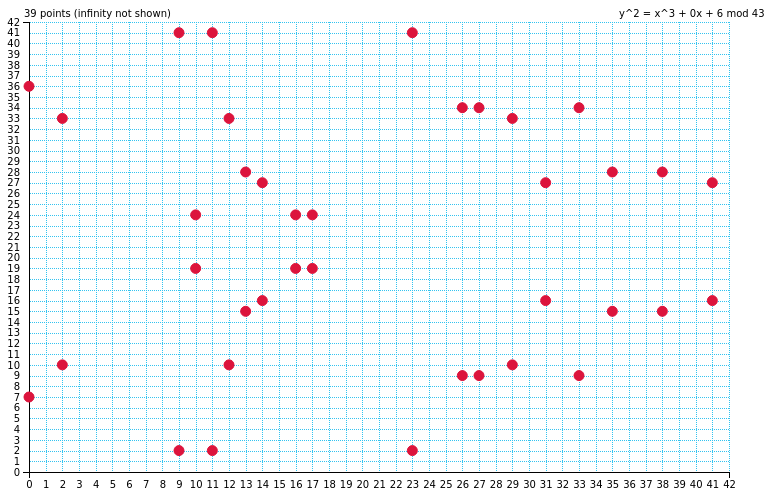
\includegraphics[scale=0.6]{figures/bls6-6.png}
As we can see our curve is somewhat nice, as it does not contain self inverse points that is points with $y=0$. It follows that the addition law can be optimized, since the branch for those cases can be eliminated. 

Note: Is there a way to printe the entire addition table from https://graui.de/code/elliptic2/ here? Would be nice to have but is a bit large.

Since the order of BLS6-6 is $39= 3\cdot 13$, we know that it has a "large" subgroup of order $13$ and small subgroup of order $3$. We can use XXX to find those groups. We have $BLS6-6(3)=\{\mathcal{O},(0,7),(0,36)\}$.

In addition we have the generator $g_{BLS6}:=(13,15)$ that generates
\begin{multline}
BLS6-6(13)=\\
\{(13,15) \rightarrow (33,34) \rightarrow  (38,15) \rightarrow  (35,28) \rightarrow (26,34) \rightarrow  (27,34) \rightarrow  \\ 
(27,9)  \rightarrow  (26,9) \rightarrow  (35,15) \rightarrow  (38,28) \rightarrow  (33,9) \rightarrow (13,28) \rightarrow  \mathcal{O}\}$$
\end{multline}

Computations "in the exponent": In cryptography and in particular in snarks a lot HAPPENS IN THE EXPONENT...

To use our example to explain what this means observe that from this representation, we can deduce a map from the scalar field $\F_{13}$ to $BLS6-6(13)$ with respect to our generator. WE have
$$
[\cdot]_{(13,15)}: \F_{13} \to BLS6-6(13)\;;\; x \mapsto [x](13,15)
$$

So for example we have $[1]_{(13,15)}= (13,15)$, $[7]_{(13,15)}= (27,9)$ and $[0]_{(13,15)}= \mathcal{O}$. In particular this map is a homomorphism of groups from the additive group $\F_{13}$ to $BLS6-6(13)$. This means in particular, the the additive neutral element from $\F_{13}$ is mapped to $\mathcal{O}$ and negatives are mapped to inverses. For example $[-2]_{(13,15)}= - [2]_{(13,15)}$, since
$[-2]_{(13,15)}= [11]_{(13,15)}= (33,9) = (33,-34) = -(33,34)=
- [2]_{(13,15)}$

The map also give a visualization of the ECDL problem in $BLS6-6(13)$, which is concerned with finding solutions $x\in \F_{13}$ for the equation 
$[x]_{(13,15)}= (x,y)$ for any $(x,y) \in BLS6-6(13)$. Of course ECDL is not hard in $BLS6-6(13)$, since we can deduce the solutions easily from XXX. For example the solution to $[x]_{(13,15)}= (35,15)$ is $x=9$, since $[9](13,15)=(35,15)$.

Since $[0]_{(13,15)}$ maps the group of cyclic integers modulo $13$ onto our group $BLS6-6(13)$, we can use this to write down the group law in the following way:
\begingroup
    \fontsize{5pt}{5pt}\selectfont
$$
\begin{array}{c|ccccccccccccc}
\cdot & \mathcal{O}  & (13,15) & (33,34) & (38,15) & (35,28) & (26,34) & (27,34) & (27,9) & (26,9) & (35,15) & (38,28) & (33,9) & (13,28)\\
\hline
\\
\mathcal{O} & \mathcal{O}  & (13,15) & (33,34) & (38,15) & (35,28) & (26,34) & (27,34) & (27,9) & (26,9) & (35,15) & (38,28) & (33,9) & (13,28)\\
\\
(13,15) & (13,15) & (33,34) & (38,15) & (35,28) & (26,34) & (27,34) & (27,9) & (26,9) & (35,15) & (38,28) & (33,9) & (13,28) & \mathcal{O}\\
\\
(33,34) & (33,34) & (38,15) & (35,28) & (26,34) & (27,34) & (27,9) & (26,9) & (35,15) & (38,28) & (33,9) & (13,28) & \mathcal{O} & (13,15)\\
\\
(38,15) & (38,15) & (35,28) & (26,34) & (27,34) & (27,9) & (26,9) & (35,15) & (38,28) & (33,9) & (13,28) & \mathcal{O} & (13,15) & (33,34)\\
\\
(35,28) & (35,28) & (26,34) & (27,34) & (27,9) & (26,9) & (35,15) & (38,28) & (33,9) & (13,28) & \mathcal{O} & (13,15) & (33,34) & (38,15)\\
\\
(26,34) & (26,34) & (27,34) & (27,9) & (26,9) & (35,15) & (38,28) & (33,9) & (13,28) & \mathcal{O} & (13,15) & (33,34) & (38,15) & (35,28)\\
\\
(27,34) & (27,34) & (27,9) & (26,9) & (35,15) & (38,28) & (33,9) & (13,28) & \mathcal{O} & (13,15) & (33,34) & (38,15) & (35,28) & (26,34)\\
\\
(27,9) & (27,9) & (26,9) & (35,15) & (38,28) & (33,9) & (13,28) & \mathcal{O} & (13,15) & (33,34) & (38,15) & (35,28) & (26,34) & (27,34)\\
\\
(26,9) & (26,9) & (35,15) & (38,28) & (33,9) & (13,28) & \mathcal{O} & (13,15) & (33,34) & (38,15) & (35,28) & (26,34) & (27,34) & (27,9)\\
\\
(35,15) & (35,15) & (38,28) & (33,9) & (13,28) & \mathcal{O} & (13,15) & (33,34) & (38,15) & (35,28) & (26,34) & (27,34) & (27,9) & (26,9)\\
\\
(38,28) & (38,28) & (33,9) & (13,28) & \mathcal{O} & (13,15) & (33,34) & (38,15) & (35,28) & (26,34) & (27,34) & (27,9) & (26,9) & (35,15)\\
\\
(33,9) & (33,9) & (13,28) & \mathcal{O} & (13,15) & (33,34) & (38,15) & (35,28) & (26,34) & (27,34) & (27,9) & (26,9) & (35,15) & (38,28)\\
\\
(13,28) & (13,28) & \mathcal{O} & (13,15) & (33,34) & (38,15) & (35,28) & (26,34) & (27,34) & (27,9) & (26,9) & (35,15) & (38,28) & (33,9)\\
\end{array}
$$
\endgroup


Cofactor clearing: 

Given an arbitrary point on the curve that is not in any of our two subgroups like $(2,33)$, we can project it on both subgroups $BLS6-6(3)$ and $BLS6-6(13)$ respectively, by \textit{multiplication with the cofactor}. Since $39 = 3 \cdot 13$, we have to multiply $(2,33)$ with $13$ to map it onto $BLS6-6(3)$ and we have to multiply $(2,33)$ with $3$ to map it onto $BLS6-6(13)$. Indeed we get $[13](2,33)= (0,36)$ which is an element of $BLS6-6(3)$ and $[3](2,33)= (35,15)$ which is an element of $BLS6-6(13)$

In what follows we want to compute type 2 pairings on our BLS6 curve. We therefore need to extract the subgroup $\mathbb{G}_1$ as well as $\mathbb{G}_2$ from the full $13$-torsion group. We already know from XXX that $\mathbb{G}_1$ is given by  
\begin{multline*}
\mathbb{G}_1=\{(13,15) \rightarrow (33,34) \rightarrow  (38,15) \rightarrow  (35,28) \rightarrow (26,34) \rightarrow  (27,34) \rightarrow  \\ 
(27,9)  \rightarrow  (26,9) \rightarrow  (35,15) \rightarrow  (38,28) \rightarrow  (33,9) \rightarrow (13,28) \rightarrow  \mathcal{O}\}$$
\end{multline*}

In type 2 pairings, the group $\mathbb{G}_2$ is defined by those elements $P$ of the full $13$-torsion group, that are mapped to $43\cdot P$ under the Frobenius endomorphism XXX. Since $BLS6/\F_{13^6}$ contains $6321251664$ elements, we can not simply loop through all elements, to find the full $13$-torsion group and extract all elements from $\mathbb{G}_2$. However we can derive the full $13$-torsion as the set of all $13$-division points and then extract $G_2$ from this
\begin{sagecommandline}
sage: F43 = GF(43)
sage: F43t.<t> = F43[]
sage: F43_6.<v> = GF(43^6, name='v', modulus=t^6+6) # t^6+6 irreducible
sage: BLS6 = EllipticCurve (F43_6,[0 ,6])
sage: INF = BLS6(0) # point at infinity
sage: for P in INF.division_points(13): # PI(P) == [q]P
....:     if P.order() == 13: # exclude point at infinity
....:         PiP = BLS6([a.frobenius() for a in P])
....:         qP = 43*P
....:         if PiP == qP:
....:             print(P.xy())
\end{sagecommandline}

Choose $g_2=(7v^2, 16v^3)$ as generator of $\mathbb{G}_2$, we get
\begin{multline*}
\mathbb{G}_2=\{
(7v^2, 16v^3) \to
(10v^2, 28v^3)\to
(42v^2, 16v^3)\to
(37v^2, 27v^3)\to\\
(16v^2, 28v^3)\to
(17v^2, 28v^3)\to
(17v^2, 15v^3)\to
(16v^2, 15v^3)\to\\
(37v^2, 16v^3)\to
(42v^2, 27v^3)\to
(10v^2, 15v^3)\to
(7v^2, 27v^3)\to
\mathcal{O}\}
\end{multline*}
e.g. $[3]g_2= (42v^2, 16v^3)$.

Having those groups we can do pairings. We choose the Weil pairing and invoke sagemath. For example the Weil pairing between our two generators is
$$
e(g_1,g_2)= 5v^5 + 16v^4 + 16v^3 + 15v^2 + 3v + 41
$$

\begin{sagecommandline}
sage: g1 = BLS6([13,15])
sage: g2 = BLS6([7*v^2, 16*v^3])
sage: g1.weil_pairing(g2,13)
\end{sagecommandline}

As we have seen, $\mathbb{G}_2$ needs quite a bit more storage space then $\mathbb{G}_1$, since elements in $\mathbb{G}_2$ are pairs of polynomials of degree $<6$ with coefficients in $\F_{43}$, while elements from $\mathbb{G}_1$ are just pairs of elements from $\F_{43}$. 

As we know from XXX it is possible to reduce the space needed to store $\mathbb{G}_2$ by using the concept of a twist. In our case $BLS6$ has embedding degree $6$ and the curve parameter $a$ in $y^2 = x^3 +ax + b$ is zero. We therefore know from XXX, that BLS6 has three different twist: A quadratic twist, a cubic twist and a sextic twist. We want to compute all of these twist:

The quadratic twisted BLS6-6 curve: Consider our BLS6-6 curve $BLS6-6/\F_{43^6}$. A quadratic twist is then another curve $BLS6-6_{2-twist}$ over $\F_{43^3}$ isomorphic to the original curve. We use XXX. The task is to find an $\omega\in \F_{43^6}$, such that $\omega^2 \in \F_{43^3}$. 
We choose $\omega = x^4 + 7x^3 + 9x^2 + 11x + 8$. Then we interpret $\delta = \omega^2 = 27x^2 + 17x + 35$ as an element from $\F_{43^3}$. So our twisted curve is
$y^2 = x^3+a\delta^2 x+b \delta^3 = x^3+6\cdot(27t^2+17t+35)$
so we get
$$
BLS6-6_{2-twist}/\F_{43^3}: y^2 = x^3+(10t^2+14t+15)
$$

\subsection{MNT4 MNT6 Cycles}
% https://eprint.iacr.org/2006/372.pdf theorem 5.2
\begin{theorem}
Let $q$ be a prime and $E/\F_q$ be an ordinary elliptic curve such that $r= |E(Fq)|$ is a prime greater than $3$.  
\begin{itemize}
\item $E$ has embedding  degree $k= 4$ if and only if there  exists $x\in \mathbb{Z}$ such  that $t=-x$ or $t=x+1$, and $q=x^2+x+1$.\item $E$ has  embedding  degree $k= 6$ if and only if there  exists $x\in \Z$ such that $t= 1\pm 2x$ and $q=4x^2+1$.
\item There is an elliptic curve $E/\F_q$ with embedding degree $6$, discriminant $D$, and $|E(Fq)| = r$ if and only if there is an elliptic curve $E'/\F_r$ with embedding degree $4$, discriminant $D$, and $|E'(\F_r)| =q$.
\end{itemize}
\end{theorem}

We can use this theorem to find an MNT6-MNT4 cycle over very small prime fields with characteristics $>3$: 
\paragraph{MNT4}
For our MNT4 curve, we can choose $x=2$. Then $q=7$ and if we choose $t= x+1 $ then $r = q + 1 - t = 7 + 1 -3 = 5$. Therefore our MNT4 curve is a curve $y^2=x^3+ax+b$ defined over $\F_7$ that consists of $5$ points. 

To construct the actual curve we could use the complex multiplication method again, but since the parameters $a$ and $b$ are from $\F_7$ there are only $48$ possibilities so we simply loop through all possible $a$'s and $b$'s and count the curve points until we find a curve that has $5$ rational points. We get
$$
y^2 = x^3 + 4x + 1
$$
defined over $\F_7$, with scalar field $\F_5$. Since $7= 2^2+2+1$, we know from theorem XXX, that this curve has embedding degree $4$ and hence qualifies as a pen\&{}paper pairing friendly elliptic curve. Since the curve's order is a prime and therefore has no non trivial factors, it has no non trivial subgroups. The curve has the following set of elements
$$MNT4=\{(0,1)\to (0,6)\to (4,2)\to (4,5) \to \mathcal{O}\}$$ 
\begin{sagecommandline}
sage: F7 = GF(7)
sage: MNT4 = EllipticCurve (F7,[4 ,1])
sage: [P.xy() for P in MNT4.points() if P.order() > 1]
\end{sagecommandline}
The multiplication table is
\begingroup
    \fontsize{10pt}{10pt}\selectfont
$$
\begin{array}{c|ccccc}
\cdot & \mathcal{O} & (0,1) & (4,5) & (4,2) & (0,6)\\
\hline
\\
\mathcal{O} & \mathcal{O} & (0,1) & (4,5) & (4,2) & (0,6)\\
\\
(0,1) & (0,1) & (4,5) & (4,2) & (0,6) & \mathcal{O}\\
\\
(4,5) & (4,5) & (4,2) & (0,6) & \mathcal{O} & (0,1)\\
\\
(4,2) & (4,2) & (0,6) & \mathcal{O} & (0,1) & (4,5)\\
\\
(0,6) & (0,6) & \mathcal{O} & (0,1) & (4,5) & (4,2)\\
\end{array}
$$
\endgroup
In what follows we choose our generator to be $g_{MNT4}=(0,1)$.

In what follows we want to compute type 2 pairings on our MNT4 curve. We therefore need to extract the subgroup $\mathbb{G}_1$ as well as $\mathbb{G}_2$ from the full $5$-torsion group. Since the order of MNT4 is a prime number, we already know from XXX that $\mathbb{G}_1$ is given by  
$$\mathbb{G}_1=\{(0,1)\to (0,6)\to (4,2)\to (4,5) \to \mathcal{O}\}$$ 

In type 2 pairings, the group $\mathbb{G}_2$ is defined by those elements $P$ of the full $5$-torsion group, that are mapped to $7\cdot P$ under the Frobenius endomorphism XXX. Since $MNT4/\F_{7^4}$ only contains $2475$ elements, we can  loop through all elements, to find the full $5$-torsion group and extract all elements from $\mathbb{G}_2$:
\begin{sagecommandline}
sage: F7t.<t> = F7[]
sage: F7_4.<u> = GF(7^4, name='u', modulus=t^4+t+1) # embedding degree is 4
sage: MNT4 = EllipticCurve (F7_4,[4 ,1])
sage: INF = MNT4(0) # point at infinity
sage: for P in INF.division_points(5): # PI(P) == [q]P
....:     if P.order() == 5: # exclude point at infinity
....:         PiP = MNT4([a.frobenius() for a in P])
....:         qP = 7*P
....:         if PiP == qP:
....:             print(P.xy())
\end{sagecommandline}

Choose $g_2=(2u^3 + 5u^2 + 4u + 2, 2u^3 + 3u + 5)$ as generator of $\mathbb{G}_2$, we get
\begin{multline*}
\mathbb{G}_2=\{ 
(2u^3 + 5u^2 + 4u + 2, 2u^3 + 3u + 5) \to
(5u^3 + 2u^2 + 3u + 6, 2u^2 + 3u) \to \\
(5u^3 + 2u^2 + 3u + 6, 5u^2 + 4u) \to
(2u^3 + 5u^2 + 4u + 2, 5u^3 + 4u + 2)\to
\mathcal{O}\}
\end{multline*}
e.g. $[3]g_2= (5u^3 + 2u^2 + 3u + 6, 5u^2 + 4u)$.

Having those groups we can do pairings. We choose the Weil pairing and invoke sagemath. For example the Weil pairing between our two generators is
$$
e(g_1,g_2)= 5u^3 + 2u^2 + 6u
$$
\begin{sagecommandline}
sage: g1 = MNT4([0,1])
sage: g2 = MNT4(2*u^3 + 5*u^2 + 4*u + 2, 2*u^3 + 3*u + 5)
sage: g1.weil_pairing(g2,5)
\end{sagecommandline}
The full pairing table can the be written as
\begingroup
    \fontsize{10pt}{10pt}\selectfont
    
% generate the table entries as:
% sage: for i in range(5):
% ....:     for j in range(5):
% ....:         p = (i*g1).weil_pairing((j*g2),5)
% ....:         print('e([',i,']g1,[',j,']g2=',p)         
    
    
$$
\begin{array}{c|lllll}
e(\cdot,\cdot)    & \mathcal{O} & g_1            & [2]g_1         & [3]g_1         & [4]g_1\\
\hline
\\
      \mathcal{O} & 1           & 1              & 1              & 1              & 1\\
\\
              g_2 & 1           & 5u^3+2u^2+6u   & 6u^3+5u^2+6    & 2u^3+u^2+2u+3  & u^3+6u^2+6u+4\\
\\
\left[2\right]g_2 & 1           & 6u^3+5u^2+6    & u^3+6u^2+6u+4  & 5u^3+2u^2+6u   & 2u^3+u^2+2u+3\\
\\
\left[3\right]g_2 & 1           & 2u^3+u^2+2u+3  & 5u^3+2u^2+6u   & u^3+6u^2+6u+4  & 6u^3+5u^2+6\\
\\
\left[4\right]g_2 & 1           & u^3+6u^2+6u+4  & 2u^3+u^2+2u+3  & 6u^3+5u^2+6    & 5u^3+2u^2+6u\\
\end{array}
$$
\endgroup

\paragraph{MNT6}
For our MNT6 curve, we can choose $x=1$. Then $q=5$ and if we choose $t= 1 + 2x $ then $r= q + 1 - t = 5 + 1 + 1 = 7$. Therefore our MNT6 curve is a curve $y^2=x^3+ax+b$ defined over $\F_5$ that consists of $7$ points. 

To construct the actual curve we could use the complex multiplication method again, but since the parameters $a$ and $b$ are from $\F_5$ there are only $24$ possibilities, we simply loop through all possible $a$'s and $b$'s and count the curve points until we find a curve that has $7$ rational points. We get
$$
y^2 = x^3 + 2x + 1
$$
defined over $\F_5$. Since $5= 4\cdot 1 + 1$, we know from theorem XXX, that this curve has embedding degree $6$ and hence qualifies as a pen\&{}paper pairing friendly elliptic curve. 

The curve has the following set of elements
$$MNT6=\{(1,2)\to (3,3)\to (0,1)\to (0,4)\to (3,2)\to (1,3)\to \mathcal{O}\}$$
The multiplication table is
\begingroup
    \fontsize{10pt}{10pt}\selectfont
$$
\begin{array}{c|ccccccc}
\cdot & \mathcal{O} & (1,2) & (3,3) & (0,1) & (0,4) & (3,2) & (1,3)\\
\hline
\\
\mathcal{O} & \mathcal{O} & (1,2) & (3,3) & (0,1) & (0,4) & (3,2) & (1,3)\\
\\
(1,2) & (1,2) & (3,3) & (0,1) & (0,4) & (3,2) & (1,3) & \mathcal{O}\\
\\
(3,3) & (3,3) & (0,1) & (0,4) & (3,2) & (1,3) & \mathcal{O} & (1,2)\\
\\
(0,1) & (0,1) & (0,4) & (3,2) & (1,3) & \mathcal{O} & (1,2) & (3,3)\\
\\
(0,4) & (0,4) & (3,2) & (1,3) & \mathcal{O} & (1,2) & (3,3) & (0,1)\\
\\
(3,2) & (3,2) & (1,3) & \mathcal{O} & (1,2) & (3,3) & (0,1) & (0,4)\\
\\
(1,3) & (1,3) & \mathcal{O} & (1,2) & (3,3) & (0,1) & (0,4) & (3,2)\\
\end{array}
$$
\endgroup

In what follows we choose our generator to be $g_{MNT6}=(1,2)$.

In what follows we want to compute type 2 pairings on our MNT6 curve. We therefore need to extract the subgroup $\mathbb{G}_1$ as well as $\mathbb{G}_2$ from the full $7$-torsion group. Since the order of MNT6 is a prime number, we already know from XXX that $\mathbb{G}_1$ is given by
$$\mathbb{G}_1=\{(1,2)\to (3,3)\to (0,1)\to (0,4)\to (3,2)\to (1,3)\to \mathcal{O}\}$$
In type 2 pairings, the group $\mathbb{G}_2$ is defined by those elements $P$ of the full $7$-torsion group, that are mapped to $5\cdot P$ under the Frobenius endomorphism XXX. Since $MNT6/\F_{5^6}$ contains $15680$ elements, we can still loop through all elements, to find the full $7$-torsion group and extract all elements from $\mathbb{G}_2$

\begin{sagecommandline}
sage: G.<x> = GF(5^6) # embedding degree is 6
sage: MNT6 = EllipticCurve (G,[2 ,1])
sage: INF = MNT6(0) # point at infinity
sage: for P in INF.division_points(7): # PI(P) == [q]P
....:     if P.order() == 7: # exclude point at infinity
....:         PiP = MNT6([a.frobenius() for a in P])
....:         qP = 5*P
....:         if PiP == qP:
....:             print(P.xy())
\end{sagecommandline}

\begin{multline*}
\mathbb{G}_2=\{ 
(x^3+2x^2+4x,x^5+2x^4+4x^3+3x^2+3)\to
(x^5+4x^4+2x^3+3x^2+x+2,3x^4+2x^3+x)\to\\
(4x^5+x^4+2x^3,3x^5+x^4+x^3+4x+4)\to
(4x^5+x^4+2x^3,2x^5+4x^4+4x^3+x+1) \to\\
(x^5+4x^4+2x^3+3x^2+x+2,2x^4+3x^3+4x)\to
(x^3+2x^2+4x,4x^5+3x^4+x^3+2x^2+2)\to
\mathcal{O}\}
\end{multline*}
We choose the generator $g_2 = (x^3+2x^2+4x,x^5+2x^4+4x^3+3x^2+3)$

\begin{remark}
Note however that our MNT6 curve discriminant $D=-16(4a^3 + 27 b^2)= -16(4\cdot 2^3 + 27\cdot 1^2)=-944$, while our MNT4 curve has discriminsnt XXX. Hence our example curves are not those guranteed by theorem XXX. Those curve are both given by $y^2= x^3 + 2x +1$ over $\F_5$ and $\F_7$, respectively. However as both curves have the same defining equation, we rather choose examples that are visually distinguishable by their defining equations.
\end{remark}



\chapter{Zk-Proof Systems}

Some philosophical stuff about compuational models for snarks. Bounded computability...

% https://docs.zkproof.org/reference.pdf

\section{Computational Models}
Proofs are the evidence of correctness of the assertions, and people can verify the cor-rectness by reading the proof. However, we obtain much more than the correctness itself:After you read one proof of an assertion, you know not only the correctness, but also why itis correct. Is it possible to solely show the correctness of an assertion without revealing theknowledge of proofs? It turns out that it is indeed possible, and this is the topic of today’slecture: Zero Knowledge Systems.
% from http://resources.mpi-inf.mpg.de/departments/d1/teaching/ss14/gitcs/notes6.pdf

\begin{example}[Generalized factorization snark]
\label{main_example_2_1}
As one of our major running examples we want to derive a zk-SNARK for the following generalized factorization problem: 

Given two numbers $a,b\in \mathbb{F}_{13}$, find two additional numbers $x,y\in \mathbb{F}_{13}$, such that
$$
(x\cdot y) \cdot a = b 
$$
and proof knowledge of those numbers, without actually revealing them.

Of course this example reduces to the classic factorization problem (over $\F_{13}$ by setting $y=1$)

This zero knowledge system deals with the following situation: "Given two publicly known numbers $a,b \in \mathbb{F}_{13}$ a proofer can show that they know two additional numbers $x,y\in \mathbb{F}_{13}$, such that $(x\cdot y) \cdot a = b$, without actually revealing $x$ or $y$." 

Of course our choice of what information to hide and what to reveal was completely arbitrary. Every other split would also be possible, but eventually gives a different problem. 

For example the task could be to not hide any of the variables.  Such 
a system has no zero knowledge and deals with verifiable computations: "A worker can proof that they multiplied three publicly known numbers $a,b,x \in \mathbb{F}_{13}$ and that the result is $z \in \mathbb{F}_{13}$, in such a way that no verifier has to repeat the computation."
\end{example}

\subsection{Formal Languages}
Roughly speaking a formal language is nothing but a set of words, that are strings of letters taken from some alphabet and formed according to some defining rules of that language. 

In computer science, formal languages are used for defining the grammar of programming languages in which the words of the language represent concepts that are associated with particular meanings or semantics. In computational complexity theory, decision problems are typically defined as formal languages, and complexity classes are defined as the sets of the formal languages that can be parsed by machines with limited computational power. 

\begin{definition}[Formal Language]
\label{def_formal_language}
 Let $\Sigma$ be a set and $\Sigma^*$ the set of all finite strings of elements from $\Sigma$. Then a \textbf{formal language} $L$ is a subset of $\Sigma^*$. The set $\Sigma$ is called the \textbf{alphabet} of $L$ and elements from $L$ are called \textbf{words}. The rules that specify which strings from $\Sigma^*$ belong to $L$ are called the \textbf{grammar} of $L$. 

In the context of proofing systems we often call words \textbf{statements}.
\end{definition}

\begin{example}[Generalized factorization snark]
\label{main_example_2_2}
Consider example \ref{main_example_2_1} again. Definition \ref{def_formal_language} is not quite suitable yet to define the example, since there is not distinction between public input and private input.

However if we assume for the moment that the task in example \ref{main_example_2_1} is to simply find $a,b,x,y\in \F_{13}$ such that that $x\cdot y\cdot a\cdot =b$, then we can define the entire solution set as a language $L_{factor}$ over the alphabet $\Sigma = \F_{13}$. We then say that a string $w\in \Sigma^*$ is a statement in our language $L_{factor}$ if and only if $w$ consists of 4 letters $w_1,w_2,w_3,w_4$ that satisfy the equation $w_1\cdot w_2\cdot w_3 =w_4$.
\end{example}

\begin{example}[Binary strings] If we take the set $\{0,1\}$ as our alphabet $\Sigma$ and imply no rules at all to form words in this set. Then our language $L$ is the set $\{0,1\}^*$ of all finite binary strings. So for example $(0,0,1,0,1,0,1,1,0)$ is a word in this language.
\end{example}

\begin{example}[Programing Language]
\end{example}

\begin{example}[Compiler]
\end{example}



As we have seen in general not all strings from an alphabet are words in a language. So an important question is, weather a given string belongs to a language or not. 

% https://www.claymath.org/sites/default/files/pvsnp.pdf
\begin{definition}[Relation, Statement, Instance and Witness] Let $\Sigma_I$ and $\Sigma_W$ be two alphabets. Then the binary relation $R\subset \Sigma_I^* \times \Sigma_W^*$ is called a \textbf{checking relation} for the language 
$$
L_R := \{(i,w) \in \Sigma_I^* \times \Sigma_W^*\;| R(i,w)\; \}
$$ 
of all \textbf{instances} $i\in \Sigma_I^*$ and \textbf{witnesses} $i\in \Sigma_I^*$, such that the \textbf{statement} $(i,w)$ satisfies the checking relation.
\end{definition}
\begin{remark}
% https://docs.zkproof.org/reference.pdf
To summarize the definition, a statement is nothing but a membership claim of the form $x\in L$. So statements are really nothing but strings in an alphabet that adhere to the rules of a language. 

However in the context of checking relations, there is another interpretations in terms of a knowledge claim of the form "In the scope of relation R, I know a witness for instance x." This is of particular importance in the context of zero knowledge proofing systems, where the instance represents public knowledge, while the witness represents the data that is hidden (the zero-knowledge part). 

For some cases, the knowledge and membership types of statements can be informally considered interchangeable, but formally there are technical reasons to distinguish between the two notions (See for example XXX
% https://docs.zkproof.org/reference.pdf
) 
\end{remark}
\begin{example}[Generalized factorization snark]
\label{main_example_2_3}
Consider example \ref{main_example_2_1} and our associate formal language \ref{main_example_2_2}. We can define another language $L_{zk-factor}$ for that example by defining the alphabet $\Sigma_I \times \Sigma_W$ to be $\F_{13} \times \F_{13}$ and the checking relation $R_{zk-factor}$ such that
$R(i,w)$ holds if and only if instance $i$ is a two letter string $i=(a,b)$ and witness $w$ is a two letter string $w=(x,y)$, such that the equation $x\cdot y \cdot a = b$ holds. 

So to summarize four elements $x,y,a,b\in \F_{13}$ form a statement 
$((x,y),(a,b))$ in $L_{zk-factor}$ with instance $(a,b)$ and witness $x,y$, precisely if, given $a$ and $b$, the values $x$ and $y$ are a solution to the generalized factorization problem $x\cdot y \cdot a = b$.
\end{example}




\begin{example}[SHA256 relation]
ssss
\end{example}

As the following example shows checking relations and their languages are quite general and able to express in particular the class of all terminating computer programs:
\begin{example}[Computer Program] Let $A$ be a terminating algorithm that transforms a binary string of inputs in finite execution steps into a binary output string. We can then interpret $A$ as a map 
$$
A :\{0,1\}^* \to \{0,1\}^*
$$
Algorithm $A$ then defines a relation
$R\subset \{0,1\}^* \times \{0,1\}^*$ in the following way: instance string $i\in \{0,1\}^*$ and witness string $w\in \{0,1\}^*$ satisfy the relation $R$, that is $R(i,w)$, if and only if $w$ is the result of algorithm $A$ executed on input instance $i$.
\end{example}

\subsection{Circuits} 
\begin{definition}[Circuits] Let $\Sigma_I$ and $\Sigma_W$ be two alphabets. Then a directed, acyclic graph $C$ is called a \textbf{circuit} over $\Sigma_I \times \Sigma_W$, if the graph has an ordering and every node has a label in the following way:
\begin{itemize}
\item Every source node (called input) has a letter from $\Sigma_I \times \Sigma_W$ as label.
\item Every sink node (called output) has a letter from $\Sigma_I \times \Sigma_W$ as label.
\item Every other node (called gate) with $j$ incoming edges has a label that consist of a function $f: \left(\Sigma_I \times \Sigma_W\right)^j \to \Sigma_I \times \Sigma_W$.
\end{itemize}
\end{definition}
\begin{remark}[Circuit-SAT] Every circuit with $n$ input nodes and $m$ output nodes can be seen a function that transforms strings of size $n$ from $\Sigma_I \times \Sigma_W$ into strings of size $m$ over the same alphabet. The transformation is done by sending the strings from a node along the outgoing edges to other nodes. If those nodes are gates, then the string is transformed according to the label.

By executing the previous transformation, every node of a circuit has an associated letter from $\Sigma_I \times \Sigma_W$ and this defines a checking relation over $\Sigma_I^* \times \Sigma_W^*$. To be more precise, let $C$ be a circuit with $n$ nodes and $(i,w) \in \Sigma_I^j \times \Sigma_W^k$ a string. Then $R_C(i,w)$ iff THE CIRCUIT IS SATISFIED WHEN ALL LABELS ARE ASSOCIATED TO ALL NODES IN THE CIRCUIT.... BUT MORE PRECISE

MODULO ERRORS. TO BE CONTINUED.....

An Assignment associates field elements to all edges (indices) in an algebraic circuit. An Assignment is valid, if the field element arise from executing the circuit. Every other assignment is invalid.

The checking relation for circuit-SAT then is satidfied if valid asignment (TODO: THE WITNESS/INSTANCE SPLITTING)

Valid assignments are proofs for proper circuit execution.
\end{remark}



So to summarize, algebraic circuits (over a field $\mathbb{F}$) are directed acyclic graphs, that express arbitrary, but bounded computation. Vertices with only outgoing edges (leafs, sources) represent inputs to the computation, vertices with only ingoing edges (roots, sinks) represent outputs from the computation and internal vertices represent field operations (Either addition or multiplication). It should be noted however that there are many circuits that can represent the same laguage...

Circuits have a notion of execution, where input values are send from leafs along edges, through internal vertices to roots.

\begin{remark}
Algebraic circuits are usually derived by  Compilers, that transform  higher languages to circuits. An example of such a compiler is XXX. Note: Different Compiler give very different circuit representations and Compiler optimization is important.
\end{remark}


\begin{example}[Generalized factorization snark]
\label{main_example_2_4}
Consider our generalized factorization example \ref{main_example_2_1} with associated language \ref{main_example_2_3}.

To write this example in circuit-SAT, consider the following function 
\[
f:\mathbb{F}_{13}\times\mathbb{F}_{13}\times\mathbb{F}_{13}\to\mathbb{F}_{13};(x_{1},x_{2},x_{3})\mapsto(x_{1}\cdot x_{2})\cdot x_{3}
\]

A valid circuit for $f:\mathbb{F}_{11}\times\mathbb{F}_{11}\times\mathbb{F}_{11}\to\mathbb{F}_{11};(x_{1},x_{2},x_{3})\mapsto(x_{1}\cdot x_{2})\cdot x_{3}$ is given by:

\[
\xymatrix{\star\ar^{in_1}[dr] &  & \star\ar_{in_2}[dl]\\
 & \star_{m_1}\ar^{mid_1}[drr] &   & & \star\ar_{in_3}[dl]\\
  &  &  & \star_{m_2}\ar_{out_1}[d]\\
  &  &  & \star
}
\]
with edge-index set $I:=\{in_{1},in_{2},in_{3},mid_{1},out_{1}\}$.

To given a valid assignment, consider the set $I_{valid}:=\{in_{1},in_{2},in_{3},mid_{1},out_{1}\} = \{2,3,4,6,10\}$

\[
\xymatrix{\star\ar^{2}[dr] &  & \star\ar_{3}[dl]\\
 & \star_{m_1}\ar^{6}[drr] &   & & \star\ar_{4}[dl]\\
  &  &  & \star_{m_2}\ar_{10}[d]\\
  &  &  & \star
}
\]
Appears from multiplying the input values at $m_1$, $m_2$ in $\mathbb{F}_{13}$, hence by executing the circuit.

Non valid assignment: $I_{err}:=\{in_{1},in_{2},in_{3},mid_{1},out_{1}\} =\{2,3,4,7,8\}$
\[
\xymatrix{\star\ar^{2}[dr] &  & \star\ar_{3}[dl]\\
 & \star_{m_1}\ar^{7}[drr] &   & & \star\ar_{4}[dl]\\
  &  &  & \star_{m_2}\ar_{8}[d]\\
  &  &  & \star
}
\]
Can not appear from multiplying the input values at $m_1$, $m_2$ in $\mathbb{F}_{13}$

To match the requirements of the inital task \ref{main_example_2_1}, we have to split the statement into instance and witness. So given index set $I:=\{in_{1},in_{2},in_{3},mid_{1},out_{1}\}$, we assume that every step in the computation other then $in_3$ and $out_1$ are part of the witness. So we choose:
\begin{itemize}
\item Instance $S=\{in_3, out_1\}$. 
\item Witness $W=\{in_1, in_2, mid_{1}\}$.
\end{itemize}
\end{example}

\begin{example}[Baby JubJub for BLS6-6]

\end{example}

\begin{example}[ECDH as a circuit]
over BLS6
\end{example}

\begin{example}[BLS Signature]
example of one layer recursion over MNT4 and MNT6
\end{example}


\begin{example}[Boolean Circuits]

\end{example}

\begin{example}[Algebraic (Aithmetic) Circuits]

\end{example}

Any program  can be reduced to  an arithmetic circuit  (a circuit that contains only addition and multiplication gates). A particular reduction can be found for example in [BSCG+13]



\subsection{Rank-1 Constraint Systems}

\begin{definition}[Rank-1 Constraint system]
Let $\F$ be a Galois field, $i,j,k$ three numbers and $A$, $B$ and $C$ three $(i+j+1) \times k$ matrices with coefficients in $\F$. Then any vector $x= (1,\phi,w)\in \F^{1+i+j}$ that satisfies the \textbf{rank-1 constraint system} (R1CS)
$$
Ax \odot Bx = Cx
$$
(where $\odot$ is the Hadamard/Schur product) is called a \textbf{statement} of that system, with \textbf{instance} $\phi$ and \textbf{witness} $w$.

We call $k$ the \textbf{number of constraints}, $i$ the \textbf{instance} size and $j$ the \textbf{witness} size.
\end{definition}

\begin{remark} Any Rank-1 constraint system defines a formal language in the following way: Consider the alphabets $\Sigma_I:= \F$ and $\Sigma_W:\F$. Then a checking relation $R_{R1CS} \subset \Sigma_I^i \times \Sigma_W^j \subset \Sigma_I^* \times \Sigma_W^*$ is defined by 
$$
R_{R1CS}(i,w) \Leftrightarrow (i,w)\text{ satisfies the R1CS}
$$
As shown in XXX such a checking relation defines a formal language. We call this language \textbf{R1CS satisfiability}.
\end{remark}

\begin{example}[Generalized factorization snark]
\label{main_example_2_4}
Defining the 5-dimensional affine vector $w =(1,in_1,in_2,in_3,m_1,out_1)$ for $in_1,in_2,in_3,m_1,out_1 \in \F_{13}$ and the $6\times ?$-matrices
$$
\begin{array}{lcr}
A = \begin{pmatrix}
0 & 1 & 0 & 0 & 0 & 0 \\ 
0 & 0 & 0 & 0 & 1 & 0
\end{pmatrix}, &
B = \begin{pmatrix}
0 & 0 & 1 & 0 & 0 & 0 \\ 
0 & 0 & 0 & 1 & 0 & 0
\end{pmatrix}, &
C = \begin{pmatrix}
0 & 0 & 0 & 0 & 1 & 0 \\ 
0 & 0 & 0 & 0 & 0 & 1
\end{pmatrix} 
\end{array}
$$
We can instantiate the general R1CS equation $Aw \odot Bw = Cw$ as
$$
\begin{pmatrix}
0 & 1 & 0 & 0 & 0 & 0 \\ 
0 & 0 & 0 & 0 & 1 & 0
\end{pmatrix} 
\begin{pmatrix}
1\\ in_1 \\ in_2 \\ in_3 \\ m_1 \\ out_1 
\end{pmatrix}\odot 
\begin{pmatrix}
0 & 0 & 1 & 0 & 0 & 0 \\ 
0 & 0 & 0 & 1 & 0 & 0
\end{pmatrix} 
\begin{pmatrix}
1\\ in_1 \\ in_2 \\ in_3 \\ m_1 \\ out_1 
\end{pmatrix} =
\begin{pmatrix}
0 & 0 & 0 & 0 & 1 & 0 \\ 
0 & 0 & 0 & 0 & 0 & 1
\end{pmatrix} 
\begin{pmatrix}
1\\ in_1 \\ in_2 \\ in_3 \\ m_1 \\ out_1 
\end{pmatrix}
$$
So evaluating all three matrix products and the Hadarmat prodoct we get two constraint equations
$$
\begin{array}{rcl}
in_1 \cdot in_2  &= & m_1 \\
m_1 \cdot in_3  &= & out_1 \\
\end{array}
$$
\end{example}
So from the way this R1CS is constructed, we know that whatever the underlying field $\F$ is, the only solutions to this equations are
$$
\{(0,0,0), (0,1,0), (1,0,0), (1,1,1)\}
$$

\subsection{Quadratic Arithmetic Programs}
As shown by [Pinocchio] rank-1 constraint systems can be transformed into so called quadratic  arithmetic  programs  assuming $\F$.

taken from the pinocchio paper. For proving arithmetic circuit-sat.  Given a R1CS QAPs transform potential solution vectors into two polynomials $p$ and $t$, such that $p$ is divisible by $t$ if and only if the vector is a solution to the R1CS. 

They are major building blocks for \textbf{succinct} proofs, since with high probability, the divisibility check can be performed in a single point of those polynomials. So computationally expensive polynomial division check is reduced TO WHAT? (IN FIELDS THERE IS ALWAYS DIVISIBILITY) 
% https://courses.cs.ut.ee/MTAT.07.022/2013_fall/uploads/Main/alisa-report

\begin{definition}[Quadratic Arithmetic Program]
Assume we have a Galois field $\F$, three numbers $i,j,k$ as well as three $(i+j+1) \times k$ matrices $A$, $B$ and $C$  with coefficients in $\F$ that define the R1CS
$Ax \odot Bx = Cx $ for some statement $x=(1,i,w)$ and let $m_1,\ldots,m_k\in \F$ be arbitrary field elements. 

Then a \textbf{quadratic arithmetic program} of the R1CS is the following set of polynomials over $\F$
$$
QAP = \left\{t\in \F[x],\left\{a_h,b_h,c_h\in \F[x]\right\}_{h=1}^{i+j+1}\right\}
$$
where $t(x) := \Pi_{l=1}^k (x- m_l)$ is a polynomial f degree $k$, called the \textbf{target polynomial} of the QAP and $a_h(x)$, $b_h(x)$ as well as $c_h(x)$ are the unique degree $k-1$ polynomials that are defined by the equations
$$
\begin{array}{lllr}
a_h(m_l)=A_{h,l} & b_h(m_l)=B_{h,l} & c_h(m_l)=C_{h,l} & h= 1, \ldots , i+j+1, l=1,\ldots,k 
\end{array}
$$  
\end{definition}
The major point is that R1CS-sat can be reformulated into the divisibility of a polynomials defined by any QAP.
\begin{theorem}
Assume that an R1CS and an associated QAP as defined in XXX are given. Then the affine vector $y=(1,i,w)$ is a solution to the R1CS, if and only if the polynomial
$$
p(x) = \left(\sum y_h\cdot a_h(x)\right)\cdot \left(\sum y_h\cdot b_h(x)\right)  - \sum y_h\cdot c_h(x) 
$$
is divisible by the target polynomial $t$.
\end{theorem}

The polynomials $a_h$, $b_h$ and $c_h$ are uniquely defined by the equations in XXX. However to actually compute them we need some algorithm like the Langrange XXX from XXX.

\begin{example}[Generalized factorization snark]
In this example we want to transform the R1CS from example \ref{main_example_2_3} into an associated QAP.

We start by choosing an arbitrary field element for every constraint in the R1CS, since we have $2$ constraints we choose $m_{1}=5$ and $m_{2}=7$

With this choice we get the target polynomial $t(x)=(x-m_1)(x-m_2)= (x-5)(x-7)= (x+8)(x+6)= x^2 + x +9$.

Since our statement has structure $w=(1, in_1,in_2,in_3,m_1,out_1)$ we have to compute the following degree $1$ polynomials

$\{a_{c},a_{in_{1}},a_{in_{2}},a_{in_{3}},a_{mid_{1}},a_{out}\}$
$\{b_{c},b_{in_{1}},b_{in_{2}},b_{in_{3}},b_{mid_{1}},b_{out}\}$
$\{c_{c},c_{in_{1}},c_{in_{2}},c_{in_{3}},c_{mid_{1}},c_{out}\}$

\item Apply QAP rule XXX to the $a_{k\in I}$ polynomials gives
$$
\begin{array}{llllll}
a_{c}(5)=0, & a_{in_{1}}(5)=1, & a_{in_{2}}(5)=0, & a_{in_{3}}(5)=0, & a_{mid_{1}}(5)=0, & a_{out}(5)=0 \\
a_{c}(7)=0, & a_{in_{1}}(7)=0, & a_{in_{2}}(7)=0, & a_{in_{3}}(7)=0, & a_{mid_{1}}(7)=1, & a_{out}(7)=0\\
\\
b_{c}(5)=0, & b_{in_{1}}(5)=0, & b_{in_{2}}(5)=1, & b_{in_{3}}(5)=0, & b_{mid_{1}}(5)=0, & b_{out}(5)=0 \\
b_{c}(7)=0, & b_{in_{1}}(7)=0, & b_{in_{2}}(7)=0, & b_{in_{3}}(7)=1, & b_{mid_{1}}(7)=0, & b_{out}(7)=0\\
\\
c_{c}(5)=0, & c_{in_{1}}(5)=0, & c_{in_{2}}(5)=0, & c_{in_{3}}(5)=0, & c_{mid_{1}}(5)=1, & c_{out}(5)=0 \\
c_{c}(7)=0, & c_{in_{1}}(7)=0, & c_{in_{2}}(7)=0, & c_{in_{3}}(7)=0, & c_{mid_{1}}(7)=0, & c_{out}(7)=1
\end{array}
$$

Since our polynomials are of degree $1$ only we don't have to invoke Langrange method but can deduce the solutions right away. 

Polynomials are defined on the two values $5$ and $7$ here.
Linear Polynomial $f(x)=m\cdot x + b$ is fully determined by this. Derive the general equation:
\begin{itemize}                        
\item  $5m+b=f(5)$  and $7m+b=f(7)$  
\item  $b=f(5)-5m$ and  $b=f(7)-7m$   
\item  $b=f(5)+8m$ and  $b=f(7)+6m$  
\item  $f(5)+8m=f(7)+6m$              
\item  $8m-6m=f(7)-f(5)$               
\item  $2m=f(7)+ 12f(5)$              
\item  $7\cdot 2m=7(f(7)+12f(5))$              
\item  $m=7(f(7)+12f(5))$ 
\item             
\item  $b=f(5)+8m$                   
\item  $b=f(5)+8\cdot(7(f(7)+12f(5)))$
\item  $b=f(5)+4(f(7)+12f(5))$ 
\item  $b=f(5)+4f(7)+9f(5)$ 
\item  $b= 10f(5)+4f(7)$ 
\end{itemize}
Gives the general equation: $f(x)=7(f(7)+12f(5))x+10f(5)+4f(7)$

For $a_{in_1}$ the computation looks like this:
\begin{itemize}
\item $ a_{in_{1}}(x) = 7(a_{in_{1}}(7)+12a_{in_{1}}(5))x+ 
10a_{in_{1}}(5)+4a_{in_{1}}(7)=$
\item $7(0 + 12\cdot 1)x+ 
10\cdot 1 +4\cdot 0 =$
\item $7\cdot 12 x + 10=$
\item $6x+10$
\end{itemize}
\begin{itemize}
\item $ a_{mid_{1}}(x) = 7(a_{mid_{1}}(7)+12a_{mid_{1}}(5))x+ 
10a_{mid_{1}}(5)+4a_{mid_{1}}(7)=$
\item $7(1 + 12\cdot 0)x+ 10\cdot 0 +4\cdot 1=$
\item $7\cdot 1x +4=$
\item $7x+4 $
\end{itemize}


\begin{tabular}{|l|l|l|}\hline 
$a_{c}(x)=0 $ &$ b_{c}(x)=0   $ & $c_{c}(x)=0$ \tabularnewline\hline 
$a_{in_{1}}(x)=6x+10 $ &$ b_{in_{1}}(x)=0   $ & $c_{in_1}(x)=0$ \tabularnewline\hline 
$a_{in_{2}}(x)=0    $ &$ b_{in_{2}}(x)=6x+10$ & $c_{in_2}(x)=0$ \tabularnewline\hline 
$a_{in_{3}}(x)=0    $ &$ b_{in_{3}}(x)=7x+4$ & $c_{in_{3}}(x)=0$ \tabularnewline\hline 
$a_{mid_{1}}(x)=7x+4$ &$ b_{mid_{1}}(x)=0  $ & $c_{mid_{1}}(x)=6x+10$ \tabularnewline\hline 
$a_{out}(x)=0       $ &$ b_{out}(x)=0      $ & $c_{out}(x)=7x+4$ \tabularnewline\hline 
\end{tabular}
This gives the quadratic arithmetic program for our generalized factorization snark as
$$QAP=\{x^{2}+x+9,\{0,6x+10,0,0,7x+4,0\},\{0,0,6x+10,7x+4,0,0\},\{0,0,0,0,6x+10,7x+4\}\}$$

Now as we recall, the main point for using QAPs in snarks is the fact, that solutions to R1CS are in 1:1 correspondence to the divisibility of a polynomial $p$, constructed from a R1CS solution and the polynomials of the QAP and the target polynomial.

So lets see this in our example. We already know from example XXX, that 
$I=\{1,2,3,4,6,11\}$ is a solution to the R1CS XXX of our problem. To see how this translates to polyinomial divisibility we compute the polynomial $p_I$ by
\begin{align*}
p_I(x)& = (\sum_{h\in |I|} I_h\cdot a_h(x))\cdot 
(\sum_{h\in |I|} I_h\cdot b_h(x)) - 
(\sum_{h\in |I|} I_h\cdot c_h(x)) \\
= & (2(6x+10)+6(7x+4))\cdot(3(6x+10)+4(7x+4))-(6(6x+10)+11(7x+4)) \\
= & ((12x+7)+(3x+11))\cdot((5x+4)+(2x+3))-((10x+8)+(12x+5)) \\
= & (2x+5)\cdot(7x+7)-(9x) \\
= & (x^{2}+2\cdot7x+5\cdot7x+5\cdot7)-(9x) \\
= & (x^{2}+x+9x+9)-(9x) \\
= & x^{2}+x+9
\end{align*}
And as we can see in this particular example $p_I(x)$ is equal to the target polynomial $t(x)$ and hence it is divisible by $t$ with $p/t=1$.

To give a counter example we already know from XXX that $I=\{1,2,3,4,8, 2\}$ is not a solution to our R1CS. To see how this translates to polyinomial divisibility we compute the polynomial $p_I$ by
\begin{align*}
p_I(x)& = (\sum_{h\in |I|} I_h\cdot a_h(x))\cdot 
(\sum_{h\in |I|} I_h\cdot b_h(x)) - 
(\sum_{h\in |I|} I_h\cdot c_h(x)) \\
= & (2(6x+10)+6(7x+4))\cdot(3(6x+10)+4(7x+4))-(6(6x+10)+11(7x+4)) \\
= & 8x^{2}+11x+3
\end{align*}
This polynomial is not divisible by the target polynomial $t$ since
Not divisible by $t$: $(8x^{2}+11x+3)/(x^{2}+x+9) =8+\frac{3x+8}{x^{2}+x+9} $
\end{example}

\subsubsection{Boolean Algebra} 
% implementations can be found here: https://github.com/filecoin-project/zexe/tree/master/snark-gadgets/src/bits

Sometimes it is necessary to assume that a statement describes boolean variables. However by definition the alphabet of a statement is a finite field, which is often the scalar field of a large prime order cyclic group. So developers need a way to simulate boolean algebra inside other finite fields.

The most common way to do this, is to interpret the additive and multiplicate neutral element $\{0,1\}\subset F$ as boolean values. This is convinient because they are defined in any field. 

\paragraph{Boolean Constraint}
So when a developer needs boolean variables as part of their statement, a R1CS is required on those variables, that enforces the variable to be either $1$ or $0$. So to "constrain a field element $x\in \F$ to be $1$ or $0$ what we need is a system of equation $(A_ix)\cdot (B_ix) = C_ix$ for some $A_i,B_i,C_i\in \F$, such that the only possible solutions for $x$ are $0$ or $1$.
As it turns out such a system can be realized by a single equation
$x \cdot (1-x) =0$
We see that indeed $0$ and $1$ are the only solutions here, since for the right side to be zero, at least one factor on the left side needs to be zero and this only happens for $0$ and $1$. 

So now that we have found a correct equation for a boolean constrain, we have to translate it into the associated R1CS format, which is given by 
$$
\begin{pmatrix}0 & 1 \end{pmatrix} \begin{pmatrix} 1 \\ x \end{pmatrix}\odot
\begin{pmatrix}1 & -1 \end{pmatrix} \begin{pmatrix} 1 \\ x \end{pmatrix} =
\begin{pmatrix}0 & 0 \end{pmatrix} \begin{pmatrix} 1 \\ x \end{pmatrix}
$$
So we get $w = \begin{pmatrix} 1 \\ x\end{pmatrix}$ as well as
$A=\begin{pmatrix}0 & 1\end{pmatrix}$, $B=\begin{pmatrix}1 & -1\end{pmatrix}$ and $C=\begin{pmatrix}0 & 0\end{pmatrix}$.

Once field elements are boolean constraint, we need constraints that are able to enforce boolean algebra on them. We therefore give constraints for the functionally complete set of Boolean operators give by $AND$ and $NOT$. As all other boolean operations can be constructed from $AND$ and $NOT$, this sufficies. However in actual implementations it is of high importance to limit the number of constraints as much as possible. In reality it is therefor advantageous to implement all logic operators in constraints.   

\paragraph{AND-constraints} Given three field elements $x,y,z\in\F$ that represent boolean variables, we want to find a R1CS, such that $w=(1,x,y,z)$ satisfies the constraint system if and only if $x\; AND \; y =z$. 

So first we have to constrain $x$, $y$ and $z$ to be boolean as explained in XXX. The next thin is we need to find a R1CS that enforces the $AND$ logic. We can simply choose $x\cdot y =z$, since (for boolean constraint values) $x\cdot y$ equals $1$ if and only if both $x$ and $y$ are $1$.  

Now that we have found a correct equation for a boolean constrain, we have to translate it into the associated R1CS format, which is given by 
$$
\begin{pmatrix}0 & 1 & 0 & 0 \end{pmatrix} \begin{pmatrix} 1 \\ x \\ y \\ z \end{pmatrix}\odot
\begin{pmatrix}0 & 0 & 1 & 0 \end{pmatrix} \begin{pmatrix} 1 \\ x \\ y \\ z \end{pmatrix} =
\begin{pmatrix}0 & 0 & 0 & 1 \end{pmatrix}\begin{pmatrix} 1 \\ x \\ y \\ z \end{pmatrix}
$$
Combining this R1CS with the required fthree boolean constraints for $x$, $y$ and $z$ we get
$$
\begin{pmatrix}
0 & 1 & 0 & 0 \\
\hline
0 & 1 & 0 & 0 \\
0 & 0 & 1 & 0 \\
0 & 0 & 0 & 1 
\end{pmatrix} \begin{pmatrix} 1 \\ x \\ y \\ z \end{pmatrix}\odot
\begin{pmatrix}
0 & 0 & 1 & 0 \\
\hline
1 & -1 & 0 & 0 \\
1 & 0  & -1 & 0 \\
1 & 0 & 0 & -1 
\end{pmatrix} \begin{pmatrix} 1 \\ x \\ y \\ z \end{pmatrix} =
\begin{pmatrix}
0 & 0 & 0 & 1 \\
\hline
0 & 0 & 0 & 0 \\
0 & 0 & 0 & 0 \\
0 & 0 & 0 & 0 
\end{pmatrix}\begin{pmatrix} 1 \\ x \\ y \\ z \end{pmatrix}
$$
So from the way this R1CS is constructed, we know that whatever the underlying field $\F$ is, the only solutions to this equations are
$$
\{(0,0,0), (0,1,0), (1,0,0), (1,1,1)\}
$$
which is the set of all $(x,y,z)\in\{0,1\}^3$ such that $x\; AND\; y = z$.
\paragraph{NOT constraint}
Given two field elements $x,y\in\F$ that represent boolean variables, we want to find a R1CS, such that $w=(1,x,y)$ satisfies the constraint system if and only if $x=\lnot y$. 

So again we have to constrain $x$ and $y$ to be boolean as explained in XXX. The next think is we need to find a R1CS that enforces the $NOT$ logic. We can simply choose $(1-x) =y$, since (for boolean constraint values) this enforces that $y$ is always the boolean opposite of $x$. 

Now that we have found a correct equation for a boolean constrain, we have to translate it into the associated R1CS format, which is given by 
$$
\begin{pmatrix}1 & -1 & 0 \end{pmatrix} \begin{pmatrix} 1 \\ x \\ y \end{pmatrix}\odot
\begin{pmatrix}1 & 0 & 0 \end{pmatrix} \begin{pmatrix} 1 \\ x \\ y \end{pmatrix} =
\begin{pmatrix}0 & 0 & 1 \end{pmatrix}\begin{pmatrix} 1 \\ x \\ y \end{pmatrix}
$$
So actually we wrote the linear equation $1-x=y$ like $(1-x)\cdot 1 = y$ and translated that into the matrix equation.

Combining this R1CS with the required fthree boolean constraints for $x$, $y$ and $z$ we get
$$
\begin{pmatrix}
1 & -1 & 0 \\
\hline
0 & 1 & 0 \\
0 & 0 & 1
\end{pmatrix} \begin{pmatrix} 1 \\ x \\ y \end{pmatrix}\odot
\begin{pmatrix}
1 & 0 & 0 \\
\hline
1 & -1 & 0 \\
1 & 0  & -1 
\end{pmatrix} \begin{pmatrix} 1 \\ x \\ y \end{pmatrix} =
\begin{pmatrix}
0 & 0 & 1 \\
\hline
0 & 0 & 0 \\
0 & 0 & 0 \\
\end{pmatrix}\begin{pmatrix} 1 \\ x \\ y \end{pmatrix}
$$
So from the way this R1CS is constructed, we know that whatever the underlying field $\F$ is, the only solutions to this equations are
$$
\{(0,1), (1,0)\}
$$
which is the set of all $(x,y)\in\{0,1\}^2$ such that $x=\lnot y$.

EXERCISE: DO OR; XOR; NAND

More complicated logical constraints can then be optained by combining all sub-R1CS together. For example if the task is to enforce $(in_1\; AND \lnot in_2 ) AND in_3 = out_1$ we first apply the FLATTENING technique from XXX, which gives is
$$
\begin{array}{lcr}
\lnot in_2 &=& mid_1\\
in_1\; AND \; mid_1 &=& mid_2\\
mid_2 \; AND \; in_3 &=& out_1
\end{array}
$$
So we have the statement $w=(1,in_1,in_2,in_3, mid_1, mid_2,out_1)$, $6$ boolean constraints for the variables, $2$ constraints for the $2$ $AND$ operations and $1$ constraint for the $NOT$ operation.
\subsection{Conditional branching}

\subsubsection{UintX}
As we know circuits are not defined over integers but over finite fields instead. We therefore have no notation of integers in circuits. However on computers we also not use integers natively but Uint's instead.

\subsubsection{Curves}
Sometimes it required to do elliptic curve cryptography "inside of a circuit". This means that we have to implement the algebraic operations (addition, scalar multiplication) of an elliptic curve as a R1CS. To do this efficiently the curve that we want to implement must be defined over the same base field as the field that is used in the R1CS. 

\begin{example}
So for example when we consider an R1CS over the field $\F_{13}$ as we did in example XXX, then we need a curve that is also defined over $\F_{13}$. Moreover it is advantegous to use a (twisted) Edwards curve inside a circuit, as the addition law contains no branching (See XXX). As we have seen in XXX our Baby-Jubjub curve is an Edwards curve defined over $\F_{13}$. So it is well suited for elliptic curve cryptography in our pend and paper examples
\end{example}

\paragraph{Twisted Edwards curves constraints} As we have seen in XXX, an Edwards curve over a finite field $F$ is the set of all pairs of points $(x,y)\in \F\times \F$, such that $x$ and $y$ satisfy the equation $a\cdot x^2+y^2= 1+d\cdot x^2y^2$. 

We can interpret this equation as a constraint on $x$ and $y$ and rewrite it as a R1CS by applying the flattenin technique from XXX.
$$
\begin{array}{lcr}
x \cdot x &=& x\_sq\\
y \cdot y &=& y\_sq\\
x\_sq \cdot y\_sq &=& xy\_sq\\
(a\cdot x\_sq+y\_sq)\cdot 1 &=& 1+d\cdot xy\_sq
\end{array}
$$
So we have the statement $w=(1,x,y,x\_sq, y\_sq, xy\_sq)$ and we need 4 constraints to enforce that $x$ and $y$ are points on the Edwards curve $x^2+y^2= 1+d\cdot x^2y^2$. Writing the constraint system in matrix form, we get:
\begingroup
    \fontsize{9pt}{9pt}\selectfont
$$
\begin{pmatrix}
0 & 1 & 0 & 0 & 0 & 0 \\
0 & 0 & 1 & 0 & 0 & 0 \\
0 & 0 & 0 & 1 & 0 & 0 \\
0 & 0 & 0 & a & 1 & 0 
\end{pmatrix} \begin{pmatrix} 1 \\ x \\ y \\ x\_sq \\ y\_sq \\ xy\_sq \end{pmatrix}\odot
\begin{pmatrix}
0 & 1 & 0 & 0 & 0 & 0 \\
0 & 0 & 1 & 0 & 0 & 0 \\
0 & 0 & 0 & 0 & 1 & 0 \\
1 & 0 & 0 & 0 & 0 & 0 
\end{pmatrix}  \begin{pmatrix} 1 \\ x \\ y \\ x\_sq \\ y\_sq \\ xy\_sq \end{pmatrix} =
\begin{pmatrix}
0 & 0 & 0 & 1 & 0 & 0 \\
0 & 0 & 0 & 0 & 1 & 0 \\
0 & 0 & 0 & 0 & 0 & 1 \\
1 & 0 & 0 & 0 & 0 & d 
\end{pmatrix} \begin{pmatrix} 1 \\ x \\ y \\ x\_sq \\ y\_sq \\ xy\_sq \end{pmatrix}
$$
\endgroup
EXERCISE: WRITE THE R1CS FOR WEIERSTRASS CURVE POINTS 
\begin{example}[Baby-JubJub]
Considering our pen and paper Baby JubJub curve over from XXX, we know that the curve is defined over $\F_{13}$ and that $(11,9)$ is a curve point, while $(2,3)$ is not a curve point. 

Starting with $(11,9)$, we can compute the statement $w=(1,11,9,4,3,12)$. Substituting this into the constraints we get
$$
\begin{array}{lcr}
11 \cdot 11 &=& 4\\
9 \cdot 9 &=& 3\\
4 \cdot 3 &=& 12\\
(1\cdot 4+3)\cdot 1 &=& 1+7\cdot 12
\end{array}
$$
which is true in $\F_{13}$. So our statement is indeed a valid assignment to the twisted Edwards curve constraining system.

Now considering the non valid point $(2,3)$, we can still come up with some kind of statement $w$ that will satisfy some of the constraints. But fixing $x=2$ and $y=3$, we can never satisfy all constraints. For example $w=(1,2,3,4,9,10)$ will satisfy the first three constraints, but the last constrain can not be satisfied. Or $w=(1,2,3,4,3,12)$ will satisfy the first and the last constrain, but not the others.
\end{example}
\paragraph{Twisted Edwards curves addition} As we have seen in XXX one the major advantages of working with (twisted) Edwards curves is the existence of an addition law, that contains no branching and is valid for all curve points. Moreover the neutral element is not "at infinity" but the actual curve poin $(0,1)$.

As we know from XXX, give two points $(x_1,y_1)$ and $(x_2,y_2)$ on a twisted Edwards curve their sum is given by
$$
(x_3,y_3) = \left(\frac{x_1y_2+y_1x_2}{1+d\cdot x_1x_2y_1y_2}, \frac{y_1y_2-a\cdot x_1x_2}{1-d\cdot x_1x_2y_1y_2}\right)
$$
% https://z.cash/technology/jubjub/
We can realize this equation as a R1CS as follows: First not that we can rewrite the addition law as
$$
\begin{array}{lcl}
x_1\cdot x_2 &=& x_{12}\\
y_1\cdot y_2 &=& y_{12}\\
x_1\cdot y_2 &=& xy_{12}\\
y_1\cdot x_2 &=& yx_{12}\\
x_{12}\cdot y_{12} &=& xy_{1212}\\
x_3\cdot (1+d\cdot xy_{1212}) &=& xy_{12}+yx_{12}\\
y_3\cdot (1-d\cdot xy_{1212}) &=& y_{12}-a\cdot x_{12}
\end{array}
$$
So we have the statement $w=(1,x_1,y_1,x_2,y_2,x_3,y_3,x_{12},y_{12},xy_{12},yx_{12},xy_{1212})$ and we need 7 constraints to enforce that $(x_1,y_1)+(x_2,y_2)=(x_3,y_3)$ 
\begin{example}[Baby-JubJub]
Considering our pen and paper Baby JubJub curve over from XXX. We recall from XXX that $(11,9)$ is a generator for the large prime order subgroup. We therefor already know from XXX that
$(11,9) + (7,8) = (11,9) + [3](11,9) = [4](11,9) = (2,9)$. So we compute a valid statement as 
$w=(1,11,9,7,8,2,9,12,7,10,11,6)$. Indeed
$$
\begin{array}{lcl}
11\cdot 7 &=& 12\\
9\cdot 8 &=& 7\\
11\cdot 8 &=& 10\\
9\cdot 7 &=& 11\\
10\cdot 11 &=& 6\\
2\cdot (1+7\cdot 6) &=& 10 + 11\\
9\cdot (1-7\cdot 6) &=& 7 -1\cdot 12
\end{array}
$$
\end{example}

\paragraph{Twisted Edwards curves inversion} Similar to elliptic curves in Weierstrass form, inversion is cheap on Edwards curve as the negative of a curve point $-(x,y)$ is given by $(-x,y)$. So a curve point $(x_2,y_2)$ is the additive inverse of another curve point $(x_1,y_1)$ precisely if the equation $(x_1,y_1) = (-x_2,y_2)$ holds. We can write this as
$$
\begin{array}{lcl}
x_1 \cdot 1 &=& -x_2 \\
y_1 \cdot 1 &=& y_2
\end{array}
$$
We therefor have a statement of the form $w=(1,x_1,y_1,x_2,y_2)$ and can write the constraints into a matrix equation as
$$
\begin{pmatrix}
0 & 1 & 0 & 0 & 0 \\
0 & 0 & 1 & 0 & 0
\end{pmatrix} \begin{pmatrix} 1 \\ x_1 \\ y_1 \\ x_2 \\ y_2 \end{pmatrix}\odot
\begin{pmatrix}
1 & 0 & 0 & 0 & 0\\
1 & 0 & 0 & 0 & 0
\end{pmatrix} \begin{pmatrix} 1 \\ x_1 \\ y_1 \\ x_2 \\ y_2 \end{pmatrix} =
\begin{pmatrix}
0 & 0 & 0 & -1 & 0\\
0 & 0 & 0 & 0 & 1
\end{pmatrix} \begin{pmatrix} 1 \\ x_1 \\ y_1 \\ x_2 \\ y_2 \end{pmatrix}
$$

\paragraph{Twisted Edwards curves scalar multiplication} 

\paragraph{Curve Cycles} A particulary interesting case with far reaching implication is the situation when we have two curve $E_1$ and $E_2$, such that the scalar field of curve $E_1$ is the base field of curve $E_2$ and vice versa. In that case it is possible to implement the group laws of one curve in circuits defined over the scalar field of the other curve. 


\subsection{Quadratic span programs}

\section{proof system}
Now a \textit{proof system} is nothing but a game between two parties, where one parties task is to convince the other party, that a given string over some alphabet is a statement is some agreed on language. To be more precise. Such a system is more over \textit{zero knowledge} if this possible without revealing any information about the (parts of) that string.
\begin{definition}[(Interactive) Proofing System]
% https://link.springer.com/content/pdf/10.1007/BF00195207.pdf
Let $L$ be some formal language over an alphabet $\Sigma$. Then an \textbf{interactive proof system} for $L$ is a pair $(P,V)$ of two probabilistic interactive algorithms, where $P$ is called the \textbf{prover} and $V$ is called the \textbf{verifier}. 

Both algorithms are able to send messages to one another. Each algorithm only sees its own state, some shared initial state and the communication messages. 

The verifier is bounded to a number of steps which is polynomial in the size of the shared initial state, after which it stops in an accept state or in a reject state. We impose no restrictions on the local computation conducted by the prover. 

We require that, whenever the verifier is executed the following two conditions hold:
\begin{itemize}
\item (Completeness) If a string $x\in \Sigma^*$ is a member of language $L$, that is $x\in L$ and both prover and verifier follow the protocol; the verifier will accept.
\item (Soundness) If a string $x\in \Sigma^*$ is not a member of language $L$, that is $x\notin L$ and the verifier follows the protocol; the verifier will not be convinced.
\item (Zero-knowledge) If a string $x\in \Sigma^*$ is a member of language $L$, that is $x\in L$ and the prover follows the protocol; the verifier will not learn anything about $x$ but $x\in L$.
\end{itemize}
\end{definition}

In the context of zero knowledge proving systems definition XXX gets a slight adaptation:
\begin{itemize}
\item Instance: Input commonly known to both prover (P) and verifier (V), and used to support the statement of what needs to be proven. This common input may either be local to the prover-verifier interaction, or public in the sense of being known by external parties (Some scientific articles use "instance" and "statement" interchangeably, but we distinguish between the two.).
\item Witness: Private input to the prover. Others may or may not know something about the witness.
\item Relation: Specification of relationship between instances and witness. A relation can be viewed as a set of permissible pairs (instance, witness).
\item Language: Set of statements that appear as a permissible pair in the given relation.
\item Statement:Defined by instance and relation. Claims the instance has a witness in the relation(which is either true or false).
\end{itemize}

The following subsections define ways to describe checking relations that are particularly useful in the context of zero knowledge proofing systems

\subsection{Succinct NIZK}
Blum, Feldman and Micali
% Manuel  Blum,  Paul  Feldman,  and  Silvio  Micali.   Non-interactive  zero-knowledge  and  itsapplications.  InSTOC, pages 103–112, 1988.
 extended the notion tonon-interactivezero-knowledge(NIZK)  proofs in the  common  reference  string  model.  NIZK  proofs  are  useful  in  theconstruction of non-interactive cryptographic schemes, e.g., digital signatures and CCA-secure public key encryption.
 
\begin{definition} 
Let $\mathcal{R}$ be a relation generator that given a security parameter $\lambda$ in unary returns a polynomial time decidable binary relation $R$. For pairs $(i,w)\in R$ we call $i$ the instance\footnote{Note that in Groth16 this is called the statement. We think the term instance is more consistent with SOMETHING. } and $w$ the witness. We define $R_\lambda$ to be the set of possible relations $R$ the relation generator may output given $1^\lambda$. We will in the following for notational simplicity assume $\lambda$ can be deduced from the description of $R$. The relation generator may also output some side information, an auxiliary input $z$, which will be given to the adversary. An efficient prover publicly verifiable non-interactive argument for $R$ is a quadruple of probabilistic polynomial algorithms $(\textsc{Setup},\textsc{Prove},\textsc{Vfy},\textsc{Sim})$ such 
\begin{itemize}
\item Setup: $(CRS,\tau)\rightarrow Setup(R)$: The setup produces a common reference string $CRS$ and a simulation trapdoor $\tau$ for the relation $R$.
\item Proof: $\pi\rightarrow Prove(R,CRS,i,w)$: The prover algorithm takes as input a common reference string $CRS$ and a statement $(i,w)\in R$ and returns an argument $\pi$.
\item Verify: $0/1\rightarrow Vfy(R,CRS,i,\pi)$: The  verification algorithm  takes as input a common reference string $CRS$, an instance $i$ and an argument $\pi$ and returns 0 (reject) or 1 (accept).
\item $\pi\rightarrow Sim(R,\tau,i)$: The simulator takes as input a simulation trapdoor $\tau$ and instance $i$ and returns an argument $\pi$. 
\end{itemize}
\end{definition}

\subsubsection{Groth16}
Groth’s  constant  size  NIZK  argument  is  based  on  constructing  a  set  of  polynomial equations and using pairings to efficiently verify these equations. Gennaro, Gentry,Parno and Raykova [Pinocchio] found an insightful construction of polynomial equations based on Lagrange interpolation polynomials yielding a pairing-based NIZK argumentwith a common reference string size proportional to the size of the statement and wit-ness.

It constructs a snark  for arithmetic circuit satisfiability, where a proof consists of only 3 group elements. In addition to being small, the proof is also easy to verify. The verifier just needs to compute a number of exponentiations proportional to the instance size and check a single pairing product equation, which only  has  3  pairings.  

The  construction  can  be  instantiated  with  any  type  of  pairings including Type III pairings, which are the most efficient pairings. The argument has perfect completeness and perfect zero-knowledge. For soundness ?? 

In the common reference string model.

Setup: 
\begin{itemize}
\item random elements $\alpha,\beta,\gamma, \delta, s \in \mathbb{F}_{scalar}$ 
\item Common reference string $CRS_{QAP}$, specific to the $QAP$ and the choice of statement and witness $CRS_{QAP}= (CRS_{\mathbb{G}_1},CRS_{\mathbb{G}_2})$, with $n=deg(t)$: 
$$
CRS_{\mathbb{G}_{1}}=\left\{ \begin{array}{c}
[\alpha]g,[\beta]g,[\delta]g,\left\{ [s^{k}]g\right\} _{k=0}^{n-1},\left\{ [\frac{\beta a_{k}(s)+\alpha b_{k}(s)+c_{k}(s)}{\gamma}]g\right\} _{k\in I}\\
\left\{ [\frac{\beta a_{k}(s)+\alpha b_{k}(s)+c_{k}(s)}{\delta}]g\right\} _{k\in W},\left\{ [\frac{s^{k}t(s)}{\delta}]g\right\} _{k=0}^{n-2}
\end{array}\right\} 
$$
$$
CRS_{\mathbb{G}_{2}}=\left\{ [\beta]h ,[\gamma]h,[\delta]h,\left\{[s^k]h\right\} _{k=0}^{n-1}\right\} 
$$
\item Toxic waste: Must delete random elements after $CRS_{QAP}$ generation.
\end{itemize} 

\begin{example}[Generalized factorization snark]
\label{main_example_2_5}
In this example we want to compile our main example in Groth16. Input is the R1CS from example \ref{main_example_2_4}. We choose the following parameters

\begin{tabular}{ccccc}
\\
curve = BLS6-6 & $\mathbb{G}_1=$ BLS6-6(13) & $g = (13,15) $
& $\mathbb{G}_2=$ & $h=(7v^2,16v^3)$
\end{tabular} 

Setup phase: Recall the quadratic arithmetic program of example XXX. 

For our example we choose the following elements $\alpha=6$, $\beta=5$, $\gamma=4$, $\delta=3$, $s=2$ from $\mathbb{F}_{13}$
$$
CRS_{\mathbb{G}_{1}}=\left\{ \begin{array}{c}
[6](13,15),[5](13,15),[3](13,15),\left\{ [s^{k}](13,15)\right\} _{k=0}^{1},\left\{ [\frac{5 a_{k}(2)+6 b_{k}(2)+c_{k}(2)}{4}](13,15)\right\} _{k\in S}\\
\left\{ [\frac{5 a_{k}(2)+6 b_{k}(2)+c_{k}(2)}{3}](13,15)\right\} _{k\in W},\left\{ [\frac{s^{k}t(2)}{3}](13,15)\right\} _{k=0}^{0}
\end{array}\right\}
$$
Since we have instance indices $I=\{1, in_1,in_2\}$ and witness indices $W=\{in_3,mid_1,out_1\}$ we have 
The instance parts.
\begin{multline*}
\left[\frac{5 a_{c}(2)+6 b_{c}(2)+c_{c}(2)}{4}\right](13,15) = 
\left[\frac{5\cdot 0 +6\cdot 0 + 0 }{4}\right](13,15) =
\left[0\right](13,15) = \mathcal{O}
\end{multline*}
\begin{multline*}
\left[\frac{5 a_{in_3}(2)+6 b_{in_3}(2)+c_{in_3}(2)}{4}\right](13,15) =
\left[(5\cdot 0+6\cdot(7\cdot 2 +4)+0)\cdot 10\right](13,15) =\\
\left[(6\cdot 5 )\cdot 10\right](13,15) =
\left[1\right](13,15) =
(13,15)
\end{multline*}
\begin{multline*}
\left[\frac{5 a_{out}(2)+6 b_{out}(2)+c_{out}(2)}{4}\right](13,15) = 
\left[(5\cdot 0 +6\cdot 0 + (7\cdot 2 + 4))\cdot 10 \right](13,15) =\\
\left[5\cdot 10 \right](13,15) =
\left[11\right](13,15) = 
(33,9)
\end{multline*}

Witness part:
\begin{multline*}
\left[\frac{5 a_{in_1}(2)+6 b_{in_1}(2)+c_{in_1}(2)}{3}\right](13,15) = 
\left[(5\cdot (6\cdot 2 +10) +6\cdot 0 +0 )\cdot 9\right](13,15) = \\
\left[(5\cdot 9)\cdot 9\right](13,15) =
\left[2\right](13,15) = (33,34)
\end{multline*}
\begin{multline*}
\left[\frac{5 a_{in_2}(2)+6 b_{in_2}(2)+c_{in_2}(2)}{3}\right](13,15) = 
\left[(5\cdot 0 +6\cdot (6\cdot 2 + 10) + 0 )\cdot 9\right](13,15) = \\
\left[(6\cdot 9)\cdot 9\right](13,15) =
\left[5\right](13,15) =
(26,34)
\end{multline*}
\begin{multline*}
\left[\frac{5 a_{mid_1}(2)+6 b_{mid_1}(2)+c_{mid_1}(2)}{3}\right](13,15) = 
\left[(5\cdot (7\cdot 2 + 4) +6\cdot 0 + 0 )\cdot 9\right](13,15) = \\
\left[(5\cdot 5)\cdot 9\right](13,15) =
\left[4\right](13,15) =
(35,28)
\end{multline*}
For $\left\{\left[\frac{s^{k}t(2)}{3}\right](13,15)\right\} _{k=0}^{0}$ we get
\begin{multline*}
\left[\frac{2^{0}t(2)}{3}\right](13,15)=
[t(2)\cdot 9](13,15)= 
[(2^2+2+9)\cdot 9](13,15)= 
[5](13,15) =
(26,34)
\end{multline*}
All together, the $\mathbb{G}_1$ part of the CRS is:
$$
CRS_{\mathbb{G}_{1}}=\left\{ \begin{array}{c}
(27,34),(26,34),(38,15),\left\{(13,15),(33,34)\right\},
\left\{\mathcal{O}, (13,15), (33,9)\right\}\\
\left\{(33,34),(26,34),(35,28)\right\},
\left\{(26,34)\right\}
\end{array}\right\}
$$
To compute the $\mathbb{G}_2$ part 
$$
CRS_{\mathbb{G}_{2}}=\left\{ [5](7v^2,16v^3) ,[4](7v^2,16v^3),[3](7v^2,16v^3),\left\{[2^k](7v^2,16v^3)\right\} _{k=0}^{1}\right\} 
$$
$$
CRS_{\mathbb{G}_{2}}=\left\{ [5](7v^2,16v^3) ,[4](7v^2,16v^3),[3](7v^2,16v^3),\left\{[1](7v^2,16v^3), [2](7v^2,16v^3)\right\}\right\} 
$$
$$
CRS_{\mathbb{G}_{2}}=\left\{(16v^2,28v^3) ,(37v^2,27v^3),(42v^2,16v^3),\left\{(7v^2,16v^3), (10v^2,28v^3)\right\}\right\} 
$$

So alltogether our common reference string is 
$$
\begin{pmatrix}
\left\{ \begin{array}{c}
(27,34),(26,34),(38,15),\left\{(13,15),(33,34)\right\},
\left\{\mathcal{O}, (13,15), (33,9)\right\}\\
\left\{(33,34),(26,34),(35,28)\right\},
\left\{(26,34)\right\}
\end{array}\right\}\\
\left\{(16v^2,28v^3) ,(37v^2,27v^3),(42v^2,16v^3),\left\{(7v^2,16v^3), (10v^2,28v^3)\right\}\right\}
\end{pmatrix}
$$

The proofer phase: 

\end{example}


\chapter{Exercises and Solutions}

TODO: All exercises we provided should have a solution, which we give here in all detail. 

\bibliography{moonmath}%use `moonmath.bib` to look for references, and print bibliography at this point in the document










\title{Pairings}
\author{}
\date{}
 
\maketitle


In this chapter, we discuss \textit{pairings}, which form the basis of several zk-SNARKs and other zero knowledge proof schemes. The SNARKs derived from pairings have the advantage of constant-sized proof sizes, which is crucial to blockchains. 

We start out by defining pairings and discussing a simple application which bears some resemblance to the more advanced SNARKs. We then introduce the pairings arising from elliptic curves and describe Miller's algorithm which makes these pairings practical rather than just theoretically interesting.


\subsection{\fontsize{11}{11}\selectfont Bilinear Pairings}


\begin{Def} \normalfont For finite abelian groups $\mb{G}_1$, $\mb{G}_2$, $\mb{G}_T$, a \textit{pairing} $$\mathbf{e}:\mb{G}_1\times \mb{G}_2 \lra \mb{G}_T$$ is a map with the following properties.

\noindent 1. Bilinearity: $\mathbf{e}(x_1+x_2,y_1+y_2) = \mathbf{e}(x_1, y_2)\cdot\mathbf{e}(x_1, y_2)\cdot\mathbf{e}(x_2, y_1)\cdot\mathbf{e}(x_2, y_2)$\\ $\forall\; x_1,x_2\in \mb{G}_1,\; y_1,y_2\in \mb{G}_2$.

\noindent 2. Non-degeneracy: The image of $\mathbf{e}$ is non-trivial.

\noindent 3. Efficient computability.\end{Def}

In pairing-based cryptography, we typically work in settings where the groups $\mb{G}_1$, $\mb{G}_2$, $\mb{G}_T$ are cyclic of order $p$ for some $256$-bit prime $p$ so as to have a $128$-bit security level. Such pairings $\mathbf{e}:\mb{G}_1\times \mb{G}_2 \lra \mb{G}_T$ are classified into three types:

\noindent - Type $\mr{I}$: $\mb{G}_1 = \mb{G}_2$.

\noindent - Type $\mr{II}$: $\mb{G}_1 \neq \mb{G}_2$ but there is an \textit{efficiently computable} isomorphism between $\mb{G}_1$ and $\mb{G}_2$.

\noindent - Type $\mr{III}$: There is no \textit{efficiently computable} isomorphism between $\mb{G}_1$ and $\mb{G}_2$.

In particular, for elements $x_1,y_1\in \mb{G}_1$, $x_2,y_2\in \mb{G}_2$, we have $\ e(x_1,y_1) = \e(x_2,y_1)\in \mb{G}_T$ if and only if there exists an integer $s\in [0,p-1]$ such that $y_1 = x_1^s$ and $y_2 = x_2^s$. This simple fact is deceptively powerful and lies at the heart of several zero-knowledge proof schemes. In all of the existing pairing based SNARKs and zero knowledge proof systems, the pairings are performed by the \textit{Verifier} rather than the Prover. Thus, it is fundamentally important for the pairings to be efficient. 


At present, the only efficient pairings that we know of are those arising from (Jacobians of) hyperelliptic curves over finite fields. The most efficient of these are the ones arising from elliptic curves, i.e. hyperelliptic curves of genus one. The fact that elliptic curves - which were pivotal to cryptography even before pairings gained traction - are the best known source of pairings seems to be a happy coincidence.



\subsubsection{\fontsize{11}{11}\selectfont Cryptographic assumptions}



We state the computationally infeasible problems that the security of pairing-based SNARKs hinges on.

\begin{Ass} {\normalfont \textbf{{$n$-strong Diffie Hellman assumption:}}} Let $\mb{G}$ be a cyclic group of prime order $p$ generated by an element $g$, and let $s \in \bFp^*$. Any probabilistic polynomial-time algorithm that is given the set $\{g^{s^i}: 1\leq i\leq n \}$ can find a pair $(a, g^{1/(s+a)})\in \bFp^*\times \mb{G}$ with at most negligible probability.\end{Ass}

\begin{Ass} {\normalfont \textbf{{Knowledge of exponent (KEA) assumption:}}}. Let $\mb{G}$ be a cyclic group of prime order $p$ generated by an element $g$, and let $s \in \bFp^*$. Suppose there exists a PPT algorithm $\mc{A}_1$ that given the set $\{g^{s^i}, g^{s^i\al}: 1\leq i\leq n \}$, outputs a pair $(c_1, c_2)\in \mb{G}\times\mb{G}$ such that $c_2 = c_1^{\al}$. Then there exists a PPT algorithm $\mc{A}_2$ that, with overwhelming probability, outputs a polynomial $f(X)\in \bFp[X]$ of degree $\leq n$ such that $c_1 = g^{f(s)}$, $c_2 = g^{\al f(s)}$.\end{Ass}

The $n$-strong Diffie Hellman is a stronger assumption than the older and more battle-tested discrete logarithm assumption in elliptic curves. The KEA assumption is even younger and is unfalsifiable. This is one of the downsides to pairing-based SNARKs when compared to schemes such as Bulletproofs, DARK etc. that do not rely on pairings.

\subsubsection{\fontsize{11}{11}\selectfont Membership proofs}


As a warmup, we discuss a simple example of an application of pairings, namely set membership proofs. This could be though of as an application specific SNARK and is substantially simpler than the Groth16 Snark which we will discuss in subsequent chapters. But it shares a common structure with the more advanced SNARKs in that 

\noin - the Prover's work is dominated by elliptic curve operations and Fast Fourier transforms

\noin - the Verifier's work is dominated by elliptic curve pairings

\noin - the scheme requires a trusted setup for the common reference string (CRS), which in practice is generated via a multi-party computation

\noin - the security hinges on the KEA and strong Diffie-Hellman assumptions

We describe the setup in this section. Let $\mb{G}_1, \mb{G}_2, \mb{G}_T$ be cyclic groups of order $p$ for some prime $p$ such that there exists a pairing ${\bf{e}}:\mb{G}_1\times \mb{G}_2\lra \mb{G}_T$ which is \textit{bilinear}, \textit{non-degenerate} and \textit{efficiently computable}. Fix generators $g_1, g_2$ of the cyclic groups $\mb{G}_1, \mb{G}_2$ respectively. Then ${\bf{e}}(g_1,g_2)$ is a generator of $\mb{G}_T$. Unlike in the case of accumulators based on groups of unknown order, the (common) order of the groups is public. Instead, the secret trapdoor is an integer $s$ in the range $[1, p-1]$ which will serve as the private key. Unfortunately, the generation of the private key requires a trusted setup. This can be partially mitigated by using a secure multi-party computation. A Verifier needs to assume that at least one of the parties involved in the MPC is honest enough not to collude with the other participants. 

For a data set $\mc{D} = \{d_1,\cdots, d_n\}$, we define the accumulated digest \vs $$\mr{Acc}(\mc{D}):= g_1^{\prod\limits_{d\in \mc{D}} (d+s)} \in \mb{G}_1. \vs $$ For a subset $\mc{D}_0\sub \mc{D}$, the witness for $\mc{D}_0$ is defined by \vs $$\mr{Wit}(\mc{D}_0) := g_1^{\prod\limits_{d\in \mc{D}\setminus \mc{D}_0} (d+s)}. \vs $$ The Verifier then needs to check whether \vs $$\mr{Wit}(\mc{D}_0)^{\prod\limits_{d_0\in \mc{D}_0} (d_0+s)} = \mr{Acc}(\mc{D}).$$ Because of the bilinearity of the pairing, it is equivalent and usually more efficient to verify the following equation: \vs $${\bf{e}}\Big(\mr{Wit}(\mc{D}_0)\;,\; g_2^{\prod\limits_{d_0\in \mc{D}_0} (d_0+s)}\Big) = {\bf{e}}(\mr{Acc}(\mc{D}), g_2). \vs $$ Since none of the parties are aware of the value of $s$, it is necessary to broadcast the sets $\{g_1, g_1^s,\cdots , g_1^{s^n}\}$ and $\{g_2, g_2^s,\cdots , g_2^{s^n}\}$ to the Prover.

In the orignal bilinear accumulator scheme, the Verifier needs access to the sets $\{g_1, g_1^s,\cdots , g_1^{s^n}\}$ and $\{g_2, g_2^s,\cdots , g_2^{s^n}\}$. But we can modify the scheme so that the Verifier only needs the four points $\{g_1,g_1^s, g_2, g_2^s \}$ to verify membership or non-membership.

The exponent $\prod\limits_{d\in \mc{D}} (d+s)$ can be interpreted as a degree $n$ polynomial in the variable $s$. The coefficients of the polynomial are computed with a run time of ${\bf{O}} (n\log(n))$ using the Fast Fourier transform. Furthermore, the set $\bFp[X]$ of polynomials with $\bFp$-coefficients is a principal ideal domain whose maximal ideals are those generated by the irreducible polynomials. For a data set $\mc{D}$, the polynomial $f(X) = \prod\limits_{d\in \mc{D}}(X+d)$ is monic of degree $n = |\mc{D}|$. Let $c_i$ denote the coefficient of $X^i$, i.e. $f(X) = \sum\limits_{i=0}^n c_iX^i$. The coefficients can be computed in run time ${\bf{O}}(n\log(n))$ using the Fast Fourier transform. The elements \vs $$g_1^{f(s)} = \prod\limits_{i=0}^n (g_1^{s^i})^{c_i}\;\in\mb{G}_1\;\;,\;\;g_2^{f(s)} = \prod\limits_{i=0}^n (g_2^{s^i})^{c_i}\;\in\mb{G}_2 \vs $$ can then be computed by any party that possesses the elements $\{g_1^{s^i}, g_2^{s^i} :\; 0\leq i \leq n  \}$. The collision-resistance of the bilinear accumulator hinges on the $n$-Strong Diffie Hellman assumption. 


\begin{mdframed}\begin{Prot} \hypertarget{PoE}{ \textit{Proof of exponent for pairings}} $(\ttt{PoE})$:\end{Prot} 

\noindent \textbf{Parameters :} A pairing ${\bf{e}}: \mb{G}_1\times \mb{G}_2\lra \mb{G}_T$ of groups of prime order $p$; generators $g_1, g_2$ of $\mb{G}_1$, $\mb{G}_2$ respectively; a secret element $s\in \bFp^*$ such that the Prover possesses the elements $\{g_1^{s^i}, g_2^{s^i}:\; 0\leq i\leq n \}$ 

\noindent \textbf{Inputs:} $a,b\in \mb{G}_1$; a polynomial $f(X)\in \bFp[X]$ of degree $\leq n$

\noindent \textbf{Claim:} $a^{f(s)} = b$

\begin{enumerate}[wide, labelwidth=!, labelindent=0pt] \vs \item The Fiat-Shamir heuristic generates a challenge $\al\in \bFp^*$ (the challenge).

\noindent 2. The Prover computes a polynomial $h(X)\in  \bFp[X]$ and an element $\be\in \bFp^*$ such that $f(X) = (X+\al)h(X)+ \be$. The Prover sends $Q:= a^{h(s)}$ to the Verifier.

\noindent 3. The Verifier computes $\be:= f(X)\Mod{(X+\al)}$ and accepts if and only if the equation \vs $$\mathbf{e}(Q, g_2^{s+\al})\cdot\mathbf{e}(a, g_2^{\be})  = \mathbf{e}(b, g_2)$$ holds.\qed \end{enumerate}\end{mdframed}


\bigskip


\noin We use the last protocol to modify the proof of membership for a data set.



\begin{mdframed} \begin{Prot} Protocol for set membership.\end{Prot} 

\noindent \textbf{Parameters :} A pairing ${\bf{e}}: \mb{G}_1\times \mb{G}_2\lra \mb{G}_T$ of groups of prime order $p$; generators $g_1, g_2$ of $\mb{G}_1$, $\mb{G}_2$ respectively; a trapdoor $s\in \bFp^*$ such that the Prover possesses the elements $\{g_1^{s^i}, g_2^{s^i}:\; 0\leq i\leq n \}$ and the Verifier possesses the set $\{g_1, g_2, g_1^s, g_2^s \}$ 

\noindent \textbf{Inputs:} Data sets $\mc{D}$, $\mc{D}_0$; the accumulated digest $\mr{Acc}(D)$

\noindent \textbf{Claim:} $\mc{D}_0\sub \mc{D}$.\vspace{0.1cm}

\normalfont \noin 1. The Prover computes the polynomial $f_0(X):= \prod\limits_{d_0\in \mc{D}_0}(X+d_0)$.

\noindent 2. The Prover computes $$\mr{Wit}(\mc{D}_0) := g_1^{\prod\limits_{d\in \mc{D}\setminus \mc{D}_0} (d+s)}.$$

\noindent 3. The Prover sends the Verifier a non-interactive \verb|PoE| for the equation $\mr{Wit}(\mc{D}_0)^{f_0(s)} = \mr{Acc}(\mc{D})$.

\noindent 4. The Verifier computes $f_0(X)$ and accepts if and only if the \verb|PoE| is valid.\qed \end{mdframed}

\bigskip


\subsection{\fontsize{11}{11}\selectfont Pairings from elliptic curves}



\noin \textbf{The Weil number:} An elliptic curve over a finite field $\bF _q$ of characteristic $p$ is endowed with the endomorphism \vs $$\mr{Fr}_{_E} : E\lra E\;\;,\;\;(x,y)\lra (x^p, y^p) .$$ This endomorphism is called the \textit{Frobenius} endomorphism of $E$ and satisfies a quadratic equation $X^2 - tX + q$ for some integer $t$. This endomorphism commutes with every endomorphism of $E$. Furthermore, the Frobenius of any elliptic curve isogenous to $E$ satisfies the same quadratic equation.

A Weil $q$-integer is an algebraic integer $\al$ such that $\sigma(\al)\cdot \ov{\sigma(\al}) = q$ for every automorphism $\sigma\in \absq$. Thus, the Frobenius of an elliptic curve is a Weil $q$-integer $\pi$ such that $[\bq(\pi):\bq]\leq 2$. From Honda-Tate theory, we know that the map $E\lra \mr{Fr}_{_E}$ yields a bijection \vspace{-5mm}

\[
  \{ \text{Elliptic curves } \bFq \text{ up to isogeny}  \} \;\;\lra\;\; \left\{\begin{array}{l}
    \text{Weil } q\text{-integers } \pi \text{ such that } [\bq(\pi):\bq]\leq 2 \\ 
     \text{ up to conjugacy} 
  \end{array}\right\}
\]

\noin \textbf{Torsion subgroups:} For any integer $n$ prime to $p$, the $n$-torsion subgroup $E(\bFP)[n]$ is isomorphic to $\bz/n\bz\times \bz/n\bz$. For any prime power $p^k$, the $p^k$-torsion is either trivial or cyclic of order $p^k$. In the former case, $E$ is said to be \textit{supersingular} while in the latter case it is said to be \textit{ordinary}. 

As the etymology suggests, most elliptic curves are ordinary. In fact, up to isogeny, there is a unique supersingular elliptic curve over the algebraic closure $\bFP$. In fact, $E$ is supersingular if and only if:

\noin - its Weil number $\pi$ is an algebraic integer of degree $\leq 2$  

\noin - $\pi^k\in \bz$ for some integer $k\geq 1$. 

Clearly, such Weil numbers - and consequently supersingular curves - are rare. Since Type I and II pairings require supersingular elliptic curves, this is yet another reason to use type III pairings instead. \\
  

\noin \textbf{Endomorphisms:} For an elliptic curve $E$, an endomorphism $\phi$ of $E$ is an algebraic map $\phi:E\lra E$. The set of endomorphisms of $E$ is called the endomorphism ring of $E$ (denoted by $\End(E)$). It has the structure of a ring with no zero-divisors that is finite dimensional over $\bz$-module. The tensor product $\End^0(E):= \End(E)\otimes_{\bz}\bq$ is called the endomorphism algebra. The center of $\End(E)$ is the subring $\bz[\pi_{_E}]$. Similarly, the field $\bq(\pi_{_E})$ is the center of the division algebra $\End^0(E)$. For simplicity, we assume the field $\bFq$ has been enlarged to endure that $\End(E) = \End(E\times_{\bFq} \bFQ)$. Broadly, $\End^0(E)$ has one of two possible structures:\vspace{1mm}

\noin 1. If $E$ is ordinary, $\End^0(E) = \bq(\pi_{_E})$ and is an imaginary quadratic field in which the prime $p$ splits. Thus, $\End(E)$ is an order (not necessarily maximal) in this imaginary quadratic field.


\noin 2. If $E$ is supersingular, $\pi_{_E} = \sqrt{q} \in \bz$ and $\End^0(E)$ is the quaternion algebra $\bq_{p,\infty}$ ramified exclusively at $p$ and $\infty_{_E}$. The endomorphism ring $\End(E)$ is a maximal order in $\bq_{p,\infty}$.\\

\noin \textbf{Examples:} 1. Consider an elliptic curve \vs $$E:y^2 = x^3 + ax \vs $$ over a prime field $\bFp$ for some $a\in \bFp^*$. In addition to the endomorphisms \vs $$E\lra E\;\,\;,\; P\mapsto [n]P\;\;\;\;(n\in\bz),    \vs $$ the curve is endowed with the endomorphism \vs $$(x_1,y_1)\mapsto (x_1,y_1\cdot\sqrt{-1}). \vs $$ Thus, $E$ has action by $\bz[\sqrt{-1}]$.\vspace{1.5mm}

\noin 2. Consider an elliptic curve \vs $$E:y^2 = x^3 + a  $$ over a prime field $\bFp$ for some $a\in \bFp^*$. In addition to the scalar multiplication endomorphisms, the curve is endowed with the endomorphism \vs $$(x_1,y_1)\mapsto (x_1,y_1\cdot\zeta_3). \vs $$ Thus, $E$ has action by $\bz[\zeta_3]$. \vspace{1.5mm}

We note that we are abusing notation by using $\sqrt{-1}$ for a square root of $-1$ in $\ov{\bq}$ as well as $\bFP$. Likewise, we have denoted a cube root of unity in $\ov{\bq}$ and $\bFP$ by $\zeta_3$.\\

\noin \textbf{The embedding degree:} Let $E$ be an elliptic curve over a finite field $\bFq$  of characteristic $p$. Let $\pi$ be the Weil number associated to $E$. Then $\pi$ is an algebraic integer such that $\pi\cdot \ov{\pi} = q$ and $\pi+\ov{\pi}\in \bz$. Furthermore, the number of $\bFqk$-points on $E$ is given by $|(1-\pi^k)(1-\ov{\pi}^k)|$.


Now, suppose $\ell\neq p$ is a prime dividing $\# E(\bFq)$. This is equivalent to there existing a prime $\mfl$ of $\bq(\pi)$ lying over $\ell$ such that $\pi-1\in \mfl$. For simplicity, assume $\ell^2$ does not divide $\# E(\bFq)$, which means:

\noin - $\ell$ splits into two distinct prime ideals $\mfl$, $\ov{\mfl}$ in $\bq(\pi)$.

\noin - $\pi-1\notin \mfl^2\cup \ov{\mfl}$. 

The $\ell$-torsion group $E(\bFP)[\ell]$ is given by \vs $$ E(\bFP)[\ell] = E(\bFP)[\mfl] \oplus E(\bFP)[\ov{\mfl}] \cong \bz/\ell\bz \times \bz/\ell\bz . \vs $$ The \textit{embedding degree} of $E$ with respect to $\ell$ is the integer $k$ that satisfies one of the following equivalent conditions: \vspace{0.1cm}

\noin 1. $k$ is the smallest integer such that $q^k\equiv 1\Mod{\ell}$.

\noin 2. $k$ is the smallest integer such that $\ov{\pi}^k\equiv 1\Mod{\mfl}$ \vspace{0.5mm}


\noin 3. $k$ is the smallest integer such that all $\ell$-torsion points of $E$ are defined over the extension $\bFqk$. 

\noin 4. $\Phi_k(q)\equiv 0\Mod{\ell}$ where $\Phi_k(X)$ is the $k$-th cyclotomic polynomial.


We denote by $\mu_{\ell}(\bF _{q^k})$ the unique cyclic subgroup of $\bF _{q^k}^*$ of order $\ell$. For a randomly chosen elliptic curve $E$, the embedding degree with respect to any prime dividing $\# E(\bFq)$ is quite large. In fact, the embedding degree is of the same order of magnitude as $q$. Elliptic curves that are amenable to pairings (aka pairing-friendly curves) are rare.

We now briefly describe the pairings associated with an elliptic curve over a finite field. To this end, we first describe divisors on curves.\\ 

\subsection{\fontsize{11}{11}\selectfont Divisors}

We start out by defining divisors on elliptic curves. Most of the concepts here generalize to arbitrary smooth curves over perfect fields. But we will confine our focus to divisors on elliptic curves over finite fields.

Let $E$ be an elliptic curve over a finite $F$ with Weierstrass equation $r(X,Y) = 0$. Let $\ov{F}$ denote the algebraic closure of $F$. We denote by $E(\ov{F})$ the group of $\ov{F}$-points of $E$. 

A \textit{divisor} $D$ on $E$ is a formal sum $\slim_{P\in E}n_{D,P}(P) $ where the $n_P$ are integers that are non-zero for at most finitely many points $P$. The set of points $P$ such that $n_{D,P}\neq 0$ is called the \textit{support} of $D$ and is denoted by $\mr{supp}(D)$. The sum $\slim_{P\in E}n_{D,P}$ is called the \textit{degree} of $D$. 

The divisor $\epsilon(D):= \slim_{P\in E, n_{D,P}\geq 0} n_{D,P}P $ is called the \textit{effective} part of $D$. The divisor $D$ is said to be \textit{effective} if $\epsilon(D) = D$. Clearly, any divisor can be realized as the difference between two effective divisors.

Thus, the set of divisors on $E$ has the structure of an abelian group and is naturally endowed with an action by $\absf$. We say a divisor $D$ is defined over $K$ if $D = \sigma(D)$ for every $\sigma\in \absf$. The set of divisors defined over $F$ is denoted by $\mr{Div}_F(E)$. This is a subgroup of $\mr{Div}(E)$.

The degree zero divisors defined over $F$ form a subgroup of $\mr{Div}_F(E)$. We denote this subgroup by $\mr{Div}_F^0(E)$. The \textit{function field} of $E$ over $F$ is the field of fractions $F(E)$ of the integral domain $F[X,Y]/r(X,Y).$ The divisor of a function $f\in F(E)$ is given by $\divv(f):= \slim_{P} m_{f,P}(P)$ where $m_{f,P}$ is the multiplicity of $P$ as a zero of $f$. 

A divisor is said to be \textit{principal} if it occurs as the divisor of some rational function. The set of divisors of functions has the structure of a group. Furthermore, a divisor $D= \slim_{P\in E}m_{D,P}(P)$ is principal if and only if $\slim_{P\in E}m_{D,P} = 0$ and $\slim_{P\in E}n_{D,P}(P) = \infty_{_E}$. Thus, every principal divisor has degree zero. We denote the set of principal divisors by $\mr{Prin}(E)$. This is a subgroup of $\mr{Div}^0(E)$.

The quotient $\mr{Div}^0(E)/\mr{Prin}(E)$ is called the \textit{divisor class group} or the Picard group of $E$ and is denoted by $\mr{Pic}^0(E)$. For elliptic curves,  $\mr{Pic}^0(E)$ has a canonical isomorphism with $E$. For higher genus curves, $\mr{Pic}^0(C)$ is not in bijection with $C$ but has the structure of an \textit{abelian variety}, a protective variety with a group structure.  


For a function $f\in \bFq(E)$ and a divisor $D= \slim_{P} m_{f,P}P$ such that $D$, $(f)$ have disjoint supports, we have \vs $$f(D) = \pl_{P} f(P)^{m_{f,P}} .$$ The \textit{Weil reciprocity law} states that for non-zero functions $f$, $g$ on the curve with disjoint supports, \vs $$f((g)) = g((f)) .$$ We omit the details since that would be too great a digression but we note that this lies at the heart of many of the proofs of the pairing properties of elliptic curves.\\

For distinct points $P$, $Q$ on the curve, we denote the line passing through them by $\mc{L}_{P,Q}$ (or $\mc{L}_{Q, P}$). We denote the tangent line to the curve at the point $P$ by $\mc{L}_{P, P}$. We denote the vertical line passing through $P$ (and $-P$) by $\mc{V}_P$ (or $\mc{V}_{-P}$). \\



\noin \textbf{Pairings:} Let $E$ be an elliptic curve over a finite field $\bFq$  of characteristic $p$. Let $\pi$ be the Weil number associated to $E$. Then $\pi$ is an algebraic integer such that $\pi\cdot \ov{\pi} = q$ and $\pi+\ov{\pi}\in \bz$. Furthermore, the number of $\bFqk$-points on $E$ is given by $|(1-\pi^k)(1-\ov{\pi}^k)|$.


Now, suppose $\ell\neq p$ is a prime such that $\# E(\bFq)\in \ell\bz\setminus \ell^2\bz$. Then the $\ell$-torsion group $E(\bFP)[\ell]$ is isomorphic to $\bz/\ell\bz \times \bz/\ell\bz$ while $E(\bFq)[\ell]\cong \bz/\ell\bz$. Let $k$ be the embedding degree of $E$ with respect to $\ell$. We denote by $\mu_{\ell}(\bF _{q^k})$ the unique cyclic subgroup of $\bF _{q^k}^*$ of order $\ell$.\\

\noin \textbf{The Tate pairing:} Let $P\in E(\bFq)[\ell]$. Then there exists a rational function $f_{\ell,P}$ with divisor $(f_{\ell,P}) = \ell(P) - \ell(\infty_{_E})$. Let $Q\in E(\bFq)$ be any representative in the equivalence class\\ $E(\bF _ {q^k})/\ell \cdot E(\bF _ {q^k})$. Let $D_Q$ be a degree zero divisor defined over $\bF _ {q^k}$ that is equivalent to $(Q)-(\infty_{_E})$ but whose support is disjoint from that of $(f_{\ell,P})$. The (intermediate) Tate pairing $t_{\ell}$ is a map \vs $$t_{\ell}: E(\bF _ {q^k})[\ell]\times E(\bF _ {q^k})/\ell \cdot E(\bF _ {q^k})\;\lra\; \bF _ {q^k}^*/(\bF _ {q^k}^*)^{\ell}\;\;,\;\;(P,Q)\mapsto f_{\ell,P}(D_Q) \vs .$$ This pairing is bilinear and non-degenerate and the target group is the quotient group $\bF _ {q^k}^*/(\bF _ {q^k}^*)^{\ell}$ which is cyclic of order $\ell$. 

A shortcoming of this pairing is that it is not entirely deterministic. Different parties may compute values that coincide under this notion of equivalence   but are distinct in a stricter sense. To this end, we modify the definition by defining \vs $$T_{\ell} : E(\bF _ {q^k})[\ell]\times E(\bF _ {q^k})/\ell \cdot E(\bF _ {q^k})\;\;\lra\;\; \mu_{\ell}(\bF _ {q^k})\vs $$ \vs $$(P,Q)\;\;\mapsto\;\; t_{\ell}(P,Q)^{(q^k-1)/\ell} = f_{\ell, P}(D_Q)^{(q^k-1)/\ell}. $$  

\noin The last part is a (rather expensive) exponentiation in the finite field $\bF _ {q^k}$ and is called the \textit{final exponentiation} for Tate pairings. It is one of the two components of a Tate pairing, the other being the Miller loops which we describe below. 



    
\bigskip



\noin \textbf{The Weil pairing:} Let $P, Q \in E(\bFqk)[\ell]$ and let $D_P$, $D_Q$ be divisors with disjoint supports such that $D_P \sim (P) - (\infty_{_E}) $, $D_Q \sim (Q) - (\infty_{_E}) $. There exist rational functions $f_{\ell,P}$, $g_{\ell,P}$ such that $(f_{\ell,P}) = \ell \cdot D_P$, $(g_{\ell,P}) = \ell \cdot D_Q$. The Weil pairing is a map \vs $$w_{\ell}: E(\bFqk)[\ell]\times E(\bFqk)[\ell]\;\lra \; \mu_{\ell}(\bFqk) $$ defined by \vs $$w_{\ell}(P,Q):= \frac{f_{\ell,P}(D_Q)}{g_{\ell,Q}(D_P)}. $$ This map is well-defined, i.e. the value $w_{\ell}(P,Q)$ is independent of the choice of the rational functions $f_{\ell,P}$, $g_{\ell,P}$. The Weil pairing is bilinear, non-degenerate and \textit{alternating} in the sense that $w_{\ell}(P,P) = 1$ for any point $P$. Furthermore, $w_{\ell}(P,Q) = 1$ if and only if $P$ and $Q$ lie in the same cyclic group of order $\ell$. Thus, choosing $r$-torsion points $P$, $Q$ that generate distinct cyclic groups $\mb{G}_1$, $\mb{G}_2$ of order $\ell$ and setting $\mb{G}_T:= \mu_{\ell}(\bFqk)$ yields a non-degenerate bilinear pairing \vs $$\e: \mb{G}_1\times\mb{G}_2 \;\lra\; \mb{G}_T . $$    

Although the Tate and Weil pairings are significantly different, their computations have a common structure. The Weil pairing boils down to computing $f_{\ell,P}(D_Q)$, $g_{\ell,P}(D_P)$ $\in \bFqk^*$. The Tate pairing entails computing $f_{\ell,P}(D_Q)\in \bFqk^*$ followed by the final exponentiation.\\


\noin \textbf{The security parameter:} The integer $\frac{\ell-1}{k}$ is called the security parameter of $E$ with respect to $\ell$. The strongest attacks against the discrete logarithm problem in the $\ell$-torsion subgroup of $E$ are 

\noin - the MOV (Menezes Okamoto Vanstone) attack which has runtime complexity $\mbf{O}\big(\frac{\ell-1}{k}).$ \\
- the Kim-Barbelescu number field sieve attack that exploits the discrete log in the target group $\bG_T$.

Thus, the integer $\frac{\ell-1}{k}$ has to be large enough for the scheme to be secure. Furthermore, $k$ has to be sufficiently large so that the index calculus attack against the DLP in $\bFqk^*$ is infeasible. On the other hand, the integer $q^k$ has to be small enough for the arithmetic in the field $\bF _{q^k}$ to be reasonably efficient. It appears that the golden mean  lies at ordinary elliptic curves with embedding degree $12$. For $128$-bit security, we need the elliptic curve to be defined over a $380$-bit prime and for the prime $\ell$ to be a $256$-bit prime.  

The curve $E$ is said to be \textit{pairing-friendly} if $\# E(\bFq)$ has a prime divisor $\ell$ such that:

\noin - $\ell\geq \sqrt{q}$\\
- the embedding degree of $E$ with respect to $\ell$ is  $\leq \log_2(\ell)/8$

In practice, the curve most widely used for SNARKs is the BLS12-381, thus named because it is defined over a $381$-bit prime field $\bFp$ and $\# E(\bFp)$ has a $256$-bit prime divisor $\ell$ such that $E$ has embedding degree $12$ with respect to $\ell$.

The BLS12-381 curve is given by the equation \vs $$E: y^2 = x^3+4 \vs $$ over a certain prime field $\bFp$ of bit-size $381$. The group $E(\bFp)$ is cyclic of order $\ell$ for a $255$-bit prime $\ell$ such that the embedding degree of $E$ with respect to $\ell$ is $12$.    The curve $E$ is ordinary and has endomorphism algebra $\bq(\sqrt{-3})$.\\


\noin \textbf{Miller's algorithm:} We now describe Miller's algorithm which allows us to compute pairings \textit{efficiently}. This elegant algorithm is the reason pairings are of practical value rather than purely of theoretical interest. A naive approach would mean $\bO(\ell)$ operations in the elliptic curve over a finite field $\bFp$, which would be impractical when $\ell \approx 2^{256}$ and $p\approx 2^{381}$. Miller's algorithm allows us to compute the parings with $\bO(\log(\ell))$  elliptic curve scalar multiplications and a final exponentiation in $\bFqk^*$.

In practice, the best optimized Tate pairing is substantially faster than the best optimized Weil pairing. Hence, we typically use Tate pairings when the     effective runtime is crucial, as is the case with blockchains.

As before, let $P$ be a point on the elliptic curve $E$. The key ingredient is to determine a function $f_{P}$ with divisor $\ell(P)-\ell(\infty_{_E})$. For every integer $i\geq 1$, the $f_{i,P}$ be a function whose divisor is \vs $$\divv(f_i) = i(P)	- ([i]P) - (i-1)(\infty_{_E}). $$ In particular, $f_{1,P} = 1$ and $f_{\ell,P} = f_{P}$. The following relation enables efficient computation of $f_{\ell,P}(D_Q)$


\begin{Lem} Let $P\in E[\ell]$ and let $i$, $j$ be integers $\geq 1$. Let $\mc{L}_{[i]P, [j]P}$ be the line through $[i]P$ and $[j]P$. Let $\mc{V}_{[i+j]P}$ be the vertical line through $[i+j]P$. Then $f_{i+j,P} = f_{i,P}f_{j,P}\frac{\mc{L}_{[i]P, [j]P}}{\mc{V}_{[i+j]P}}$.\end{Lem}


It is important to note that the degree of $f_{n,P}$ grows linearly with $n$ (en route to $\ell$). Hence, the degree of the rational function $f_{n,P}\in \bFqk(E)$ eventually becomes too large for $f_{n,P}\in \bFqk(E)$ to be stored. Miller's algorithm circumvents this bottleneck by storing the evaluation $f_{n,P}(D_Q)$ at the divisor $D_Q$ instead of storing $f_{n,P}$. 



\bigskip

\begin{mdframed} \textbf{Miller's algorithm to compute  the Tate pairing $T_{\ell}(P,Q)$} \vspace{0.15cm}

\noin \textbf{Input:} $P\in E(\bFqk)[\ell]$;\hspace{1mm} $Q  =\wti{Q}+ \ell \cdot E(\bF _ {q^k})\in E(\bF _ {q^k})/\ell \cdot E(\bF _ {q^k}) $; 

\noin $D_{Q}\sim (Q)-(\infty_{_E})$ with support disjoint from $(f_{\ell,P})$; 

\noin the binary representation $\ell = (r_{n-1}\cdots r_1 r_0)_2$ with $r_{n-1} = 1$ \vspace{0.15cm}

\noin \textbf{Output:} $f_{\ell,P}(D_Q)\gets f$ \vspace{0.15cm}

\begin{enumerate}[wide, labelwidth=!, labelindent=0pt]\vs \item $R\gets P$, $f\gets 1$

\item \textbf{for} $i = n-2$ down to $0$ do:

\item Compute the line functions $\mc{L}_{R,R}$ and $\mc{V}_{[2]R}$ for doubling $R$.

\item $R\gets [2]R$

\item $f\gets f^2\cdot \frac{\mc{L}_{R,R}}{\mc{V}_{[2]R}}(D_Q)$

\item \textbf{if} $r_i =1$ then 

\item Compute the line functions $\mc{L}_{R,P}$ and $\mc{V}_{R+P}$ for adding $R$ and $P$

\item $R\gets R+P$

\item $f\gets f\cdot \frac{\mc{L}_{R,P}}{\mc{V}_{R+P}}(D_Q)$

\item end \textbf{if}

\item end \textbf{for}

\item return $f^{(q^k-1)/{\ell}}$ \qed \end{enumerate} \end{mdframed}

\bigskip

Miller's algorithm to compute the Weil pairing has a similar structure. We can simulate Steps 1-11 to compute $f_{\ell,P}(D_Q)$, $g_{\ell,Q}(D_P))$ and then compute $\frac{f_{\ell,P}(D_Q)}{g_{\ell,Q}(D_P)} \in \mule(\bFqk^*).$






\subsection{\fontsize{11}{11}\selectfont Summary}

There is consensus that type III pairings are faster than type I and type II pairings and that Tate pairings are faster than Weil pairings. Hence, it is optimal to use a Tate pairing for an ordinary pairing-friendly elliptic curve. The curve most suitable for this purpose seems to be the BLS12-381 curve.

The fundamental computation in elliptic curve cryptography is the scalar multiplication $m\cdot P$ for an integer $m$ and an elliptic curve point $P$. This point is computed in runtime $\bO(\log(m))$ via a sequence of point doublings and point additions. One of the components of a Tate pairing is the Miller loop, which is largely an extension of the scalar multiplication computation. The other key component in a Tate pairing is the final exponentiation which is a rather expensive exponentiation operation in a finite field of size $q^k$, where $k$ is the embedding degree.  

In pairing-based SNARKs such as PLONK, Groth16 etc, the Verifier's work is dominated by pairing computations. Thus, optimizing pairings is crucial for applications of SNARKs to blockchains.











\subsection{\fontsize{11}{11}\selectfont Symbols}

\noin $(f)$: divisor of a rational function $f\in \bFP(E)$ \vspace{2mm}

\noin $\infty_{_E}$: The $E$-point at infinity \vspace{2mm}

\noin $D_P$: the divisor $(P)-(\infty_{_E})$ \vspace{2mm}

\noin $E(K)$: the group of $K$-valued points of $E$ \vspace{2mm}

\noin $E[n]$: the $n$-torsion subgroup of $E$ \vspace{2mm}

\noin $\mc{L}_{P,Q}: \begin{cases} \text{the line passing through } P \text{ and } Q \text{ if } P\neq Q\\ \text{the tangent line at } P \text{ if } P = Q \end{cases}$\vspace{2mm}

\noin $\mc{V}_{P}$: the vertical line passing through $P$ (and $-P$) \vspace{2mm}

\noin $T_{\ell}(P,Q)$: the order $\ell$ reduced Tate pairing \vspace{2mm}

\noin $t_{\ell}(P,Q)$: the intermediate order $\ell$ Tate pairing \vspace{2mm}

\noin $w_{\ell}(P,Q)$: the order $\ell$ Weil pairing  \vspace{2mm}

\noin BLS: Boneh-Lynn-Scott \vspace{2mm}

\noin $\mr{Div}(E)$: group of divisors on $E$ \vspace{2mm}

\noin $\mr{Div}_F(E)$: group of divisors on $E$ defined over $F$ \vspace{2mm}

\noin $\mr{Div}^0(E)$: group of degree zero dvisors on $E$ \vspace{2mm}

\noin $\mr{Div}^0_F(E)$: group of degree zero divisors on $E$ defined over $F$ \vspace{2mm}

\noin $\mr{ord}_P(f)$: the multiplicity of $f$ at $P$ on $E$ \vspace{2mm}

\noin $\End(E)$: The endomorphism ring of $E$  \vspace{2mm}

\noin $\End^0(E)$: The endomorphism algebra of $E$ \vspace{2mm}

\noin $\absf$: The absolute Galois group of $F$ \vspace{2mm}

\noin $\mu_{\ell}(\bFqk)$: The $\ell$-torsion of $\bFqk^*$ \vspace{2mm}

\noin $f_{n,P}$: A function with divisor $n(P)-([n]P)- (n-1)(\infty_{_E})$ \hspace{2mm} ($n\in \bz$, $P\in E(\bFqk)$) \vspace{2mm}

\noin $\mr{supp}(f)$: the support of a function $f$ \vspace{2mm}

\noin $\Phi_k(X):$ The $k$-th cyclotomic polynomial





























\end{document}